\documentclass[doctor,11pt,final]{iscs-thesis}
\usepackage[dvipdfmx]{graphicx}
\usepackage[dvipdfmx]{color}
\usepackage[ruled,noline]{algorithm2e}
\usepackage{amsmath}
\usepackage{amssymb}
\usepackage{array}
\usepackage{booktabs}
\usepackage{cleveref}
\usepackage{enumitem}
\usepackage[T1]{fontenc}
\usepackage{linguex}
\usepackage{microtype}
\usepackage{multirow}
\usepackage[round]{natbib}
\usepackage[super]{nth}
\usepackage{pifont}
\usepackage{quoting}
\usepackage{setspace}
\usepackage{tikz}
\usepackage{times}
\usepackage{xcolor,colortbl}


%% General

\renewcommand\labelitemi{\normalsize$\bullet$}

\sloppy % fix overfull errors in paragraph


%% Chapter 03
\newcommand{\utterance}[1]{``#1''}


%% Chapter 04
\definecolor{mygreen}{cmyk}{1,0,1,0.25}
\definecolor{myblue}{cmyk}{1,1,0,0}
\definecolor{myred}{cmyk}{0,1,1,0}


%% Chapter 05
\definecolor{Gray}{gray}{0.85}
\newcolumntype{a}{>{\columncolor{Gray}}c}

\newcommand{\Mod}[1]{\ (\mathrm{mod}\ #1)}


%% Chapter 06
\newcommand{\cmark}{\ding{51}}%
\newcommand{\xmark}{\ding{55}}%


%-------------------
\etitle{A Study on Advanced Common Grounding \\in Natural Language Dialogue Systems}
\jtitle{(自然言語対話システムにおける発展的な基盤化の研究)}
%
\eauthor{Takuma Udagawa}
\jauthor{宇田川拓真}
\esupervisor{Akiko Aizawa}
\jsupervisor{相澤彰子}
\supervisortitle{Professor}
\date{June 4, 2021}
%-------------------
\begin{document}
\begin{eabstract}

\begin{spacing}{1.1}
{\normalsize
One ultimate goal of natural language processing is to develop systems that can understand and communicate reliably in natural language. Towards this end, we focus on the fundamental aspect of communication called common grounding, which refers to the collaborative process of creating and maintaining mutual understandings (i.e. common ground). Despite the long history of study on this topic, we raise three major limitations in existing research. First, existing works mostly focus on restricted domains and task settings where advanced common grounding is not required. Secondly, how to evaluate and analyze common grounding remains an open problem. Finally, existing dialogue systems still have limited capability of common grounding: to be specific, traditional (pipeline) dialogue systems lack the flexibility and end-to-end (fully data-driven) systems lack the robustness required for advanced common grounding.\\
\indent To address these problems, we propose a novel research platform to study advanced common grounding in natural language communication. In Chapter \ref{01_chp:introduction}, we introduce the precise scope of this thesis, namely the viewpoint of common grounding as entity-level alignment. In Chapter \ref{02_chp:literature_review}, we give an overview of the existing literature on common grounding, dialogue systems and symbol grounding research. In Chapter \ref{03_chp:task_formulation}, we formally define the collaborative reference task to measure the ability of creating common ground. To study advanced common grounding, we propose a novel task setting under continuous and partially-observable context, where collaborative resolution of complex ambiguity, uncertainty and misunderstandings is required. Based on this task design, we developed OneCommon Corpus: a large-scale dataset of 6,760 dialogues for conducting empirical studies. In Chapter \ref{04_chp:interpretation}, we propose an annotation framework of reference resolution to interpret common grounding across modalities. We show that our approach is reliable, scalable, and useful for investigating the strategies of both humans and imperfect dialogue systems. In Chapter \ref{05_chp:analysis}, we provide additional annotation of spatial expressions on top of reference resolution. Based on these annotations, we capture fine-grained linguistic structures as well as how they are externally grounded at the level of symbol grounding. In Chapter \ref{06_chp:task_generalization}, we generalize our collaborative reference task under dynamic context to study advanced skills of maintaining common ground. Based on this task formulation, we developed Dynamic-OneCommon Corpus: another large-scale dataset containing 5,617 dialogues. Through our empirical studies, we demonstrate advanced strategies required under this setting, such as the usage of complex spatio-temporal expressions and previous common ground to retain or update common ground.\\
\indent Based on this platform, we enable various dialogue systems to be evaluated, analyzed and improved in terms of advanced common grounding. In Chapter \ref{07_chp:discussion}, we explore the future prospects of our research, including further ideas on the task design, model improvements, and real-world applications. In Chapter \ref{08_chp:conclusion}, we summarize the contributions of this thesis. Overall, we expect our study to be a fundamental step towards developing dialogue systems that can collaborate with humans reliably in natural language.
}
\end{spacing}

\end{eabstract}

\begin{jabstract}
自然言語処理研究における究極的な目標の一つは、人間のように言語を理解し、信頼性の高いコミュニケーションを行える対話システムの実現である。この目標に向けて、本論文ではコミュニケーションの根幹を成す基盤化という現象に着目する。基盤化とは、共通理解(共通基盤)を形成・維持する一連のプロセスを指し、重要な研究対象として長い歴史を持つ。しかし、既存研究には大きく三つの問題点がある。第一に、既存の対話研究はドメイン・タスク設計の観点から限られており、高度な基盤化を要請しない。第二に、基盤化の能力の評価・分析を行うことは一般に難しい。第三に、既存の対話システムの基盤化能力の限界がある。具体的には、従来の(パイプライン型の)対話システムは柔軟性に欠けており、(完全にデータ駆動型の)end-to-end 対話システムは頑健性に欠けているため、どちらも複雑な状況に対処する高度な基盤化を行うことができない。

以上の問題点を解決するために、本論文では発展的な基盤化の研究を推進するための新たな研究プラットフォームを提案する。1 章では基盤化をエンティティレベルのアラインメントとして捉えることで、本研究の対象領域の明確な導入を行う。2 章では重要な関連研究、特に基盤化・対話システム・記号接地問題の分野を概観する。3 章では正確な共通基盤の形成を評価するための協調的参照タスクを定義する。その上で、連続的な情報および部分観測的な状況を扱うタスク設定を導入することで、曖昧性・不確実性・誤解の解消を含む高度な基盤化を要請する。このタスク設定に基づき、6,760対話を含む大規模な OneCommon コーパスを構築し、様々な実証的研究を可能にする。4 章では参照解決のアノテーションに基づくモダリティ横断的な基盤化の解釈手法を提案する。提案手法によって分析の信頼性と拡張性を担保しつつ、人間だけでなく不完全な対話システムの解釈が可能になることを示す。5 章では参照解決に加えて空間表現のアノテーションを組み合わせたさらなる分析を行う。これによって対話中のより詳細な言語構造を捉えつつ、それらのモダリティ横断的な(記号接地問題のレベルでの)深い分析が可能になることを示す。6 章では協調的参照タスクを時系列的に拡張することで、動的な環境における共通基盤の維持を評価する新たなタスクの設計を行う。このタスク設計に基づき5,617対話を含む Dynamic-OneCommon コーパスを新たに構築し、動的な環境では複雑な時空間表現や過去の共通基盤を利用した高度な基盤化が要請されることを示す。

本論文の提案プラットフォームを用いることで、様々な対話システムを発展的な基盤化の観点から実装・評価・分析することが可能になる。7 章では更なるタスク設計のアイデア、モデルの改善手法、現実問題への応用を含めた今後の研究の展望について考察する。最後に 8 章では本研究全体を総括する。以上の貢献により、本論文は自然言語を通じて人間と協調できる、信頼性の高い対話システムの実現に向けた重要な基礎を構築する。

\end{jabstract}

\maketitle


\begin{acknowledge}

First and foremost, I would like to express my sincere gratitude to Professor Akiko Aizawa for her invaluable guidance. Throughout the writing of this PhD thesis, I've been always encouraged by her unwavering belief, understanding and support in my research. It was truly a life-changing experience to spend the 5 years under her supervision. I will cherish everything I've learned from her in my future career, including the virtues of modesty, kindness and respect for others.

I must also express my gratitude to Asst. Prof. Saku Sugawara for all the inspiring discussions. His pivotal insight on natural language understanding research had a profound influence on my studies. I'm also deeply grateful for always providing me constructive comments on my research plans and paper writing.

I would like to extend my sincere thanks to the members of our laboratory, especially Vitou Phy and Takato Yamazaki for willingly participating in my annotation projects. I owe my special thanks to the secretory Noriko Katsu for assisting many aspects of my laboratory life. I was fortunate to be able to work and spend the time together with all the great members at National Institute of Informatics.

I am also grateful to the members of my PhD thesis commitee, Assoc. Prof. Hideki Nakayama, Prof. Imari Sato, Prof. Masami Hagiya, Prof. Ryuichiro Higashinaka, and Prof. Yusuke Miyao. They provided me important feedback on improving the early draft and presentation of this thesis.

Finally, my deepest appreciation goes to my family: especially my parents, siblings, nephew, and partner. Without their tremendous understanding and support, this milestone could not have been achieved. I dedicate this thesis to them.

\end{acknowledge}

\frontmatter
\tableofcontents
\listoffigures
\listoftables
%-------------------
\mainmatter

\graphicspath{{01_introduction/figures/}} % Location of the graphics files

\chapter{Introduction}
\label{01_chp:introduction}

\section{The Common Grounding Problem}
\label{01_sec:common_grounding_problem}

Human communication is extraordinary. Unlike other primates, we use \textit{symbolic} natural language which can be assembled grammatically to express countless meanings, from abstract to concrete \citep{tomasello2009constructing}. Natural language is so versatile that most (if not all) of our knowledge is expressed, shared and elaborated through this medium. Hence, it is not surprising that such linguistic competence has been considered as a hallmark of human-level intelligence \citep{turing1950computing}.

But what makes human communication so reliable? At the heart of this question lies the problem of \textit{common grounding}. Common grounding is the process of creating and maintaining mutual understandings (i.e. \textit{common ground}), which is a critical aspect of sophisticated human communication. It is only through this collaborative effort that we can ensure the reliability of our shared understandings \citep{clark1996using}.

To illustrate how this process unfolds in natural language dialogues, we first introduce the \textit{contribution theory} of \citet{clark1989contributing}, which remains influential to date. According to this theory, information in dialogue transitions through 2 phases: the \textit{presentation phase}, where it gets first introduced by the speaker, followed by the \textit{acceptance phase}, where it gets acknowledged by the listener(s). It is only after the positive feedback from the listener(s) in the acceptance phase that the information is added (or \textit{contributed}) to their common ground.\footnote{Note that a piece of information can be presented in various ways, including direct assertions as well as indirect \textit{presuppositions}, e.g. implicitly assumed in a question \citep{stalnaker1978assertion}. Similarly, information can be accepted directly through acknowledgements (like ``yes'', ``okay'') or more indirectly, e.g. through the initiation of the next relevant contribution \citep{cho-may-2020-grounding}.}

To exemplify this process, we show an actual conversation reported in \citet{Sacks1974ASS}.

\ex. \label{ex_1:deictic_reference}
\a. A:\; Uh you been down \underline{here} before haven't you.
\b. B:\; Yeah.
\c. A:\; Where the sidewalk is?
\b. B:\; Yeah,
\e. A:\; Where it ends,
\f. B:\; Goes all the way up there?
\f. A:\; They come up to there, yeah.

In the first utterance (a), speaker A inquires whether B has been to the place (``\textit{here}'') before, which B recognizes and replies with a positive answer (b). These two utterances form a contribution, and the inquired fact becomes mutually accepted among A and B. However, there remains a potential ambiguity in the deictic reference ``here'', so the conversation continues to resolve it through clarifications and elaborations (c-g). Based on this process, the speakers can ensure the detail and reliability of common ground, and if there were any misunderstandings, they can be \textit{repaired} through correction (e.g. ``No, it's the \textit{opposite} side of the sidewalk.'') \citep{schegloff1977preference}.

Through the accumulation of this process, humans can develop a substantial amount of common ground foundational in various aspects of our daily life. Without the ability of reliable common grounding, the productive, stable and efficient collaboration in complex human society is unimaginable to be achieved.

%which plays a fundamental role in productive, efficient and reliable collaboration.% \citep{grosz1996collaborative,clark1996using}.

\section{Limitations of Existing Research}
\label{01_sec:existing_research}

The previous discussion corroborates the importance of common grounding in human communication. But how is this problem being addressed in the fields of artificial intelligence (AI) and natural language processing (NLP), and what are the main challenges that hinder its progress? Despite the long history of study on this topic, we raise three major limitations of existing research.

\subsubsection{Limitation on the Task Settings}

In dialogue research, \textit{task design} is an important factor that determines the subject of study (e.g. the complexity and requisite strategy of common grounding). However, existing dialogue tasks mostly focus on restricted domains and task settings where advanced, full-fledged common grounding is not required. To be specific, most existing tasks only need to deal with the following types of information which make the requisite skills of common grounding relatively trivial.

\begin{itemize}
\item \textit{Categorical} information: Traditionally, the type of information that dialogue systems handle has been limited to categorical/discrete information. For instance, the information of color would be discretized into predefined categories (e.g. ``red'', ``blue'', ``green'', and so forth) so that they can be treated with structured databases and frame-based dialogue state tracking \citep{Henderson2015}.

However, this setting ignores the aspect of many concepts being gradable and unbounded \citep{Lakoff87,paradis_2008} and introduces minimal ambiguity or uncertainty to be dealt with symbolic natural language. Consequently, they require minimal effort of semantic coordination (e.g. disambiguations and clarifications) in the process of common grounding.

\item \textit{Fully-observable} information: It is also common in prior works to assume that the information is fully-observable, i.e. all agents have the same, complete information of the environment. For instance, agents often have identical observations (e.g. the same set of images) to discuss in the dialogue \citep{zarriess-etal-2016-pentoref,de2017guesswhat,shore-etal-2018-kth}.

However, this assumption is unrealistic in many situations where we only have partial, private information of the environment. Due to the lack of such information asymmetry, existing settings introduce minimal misunderstandings or partial understandings that need to be resolved through common grounding.

\item \textit{Static} information: Finally, existing dialogue tasks mostly focus on static information and environments that do not change over time. For instance, dialogue contexts like databases \citep{he2017learning}, images \citep{haber-etal-2019-photobook} and embodied environments \citep{de2018talk,thomason:corl19} are usually assumed to be fixed/stationary in the course of the dialogue.

However, real-world environments are \textit{dynamic} and require continuous effort of maintaining common ground. In the static settings of existing works, there are minimal requirements for updating common ground and adapting to the evolving situations, e.g. by replacing old information with the new ones.

\end{itemize}

\subsubsection{Limitation on the Evaluation and Analysis}

Secondly, how to evaluate and analyze common grounding largely remains an open problem.
One main difficulty of evaluation is that systems can \textit{imitate} common grounding without actual understandings, either through simple acknowledgements and paraphrasing \citep{weizenbaum1966eliza} or based on more elaborate human-like responses \citep{adiwardana2020towards,roller-etal-2021-recipes}. Such deceptive behaviors could be misleading or even harmful to promote research on reliable common grounding. Another difficulty is the existence of \textit{dataset biases}. In the process of dataset creation, there could be various sources of suprious, unintended biases \citep{goyal2017making,gururangan-etal-2018-annotation,geva-etal-2019-modeling} which can be exploited by the models to succeed without employing the genuine, intended abilities \citep{geirhos2020shortcut}. To overcome these limitations, we need more objective, quantitative and faithful evaluation metrics to measure and propel our real progress on advanced common grounding.

In terms of analysis, there are various factors that make the analysis of common grounding difficult or problematic in realistic settings. For instance, the application of \citeauthor{clark1989contributing}'s theory may not be straightforward when contributions are implicit, indirect, unstructured, partial, etc. To illustrate this, we use another example from \citet{Sacks1974ASS}, following the explanations of \citet{lascarides2009agreement}.

\ex. \label{ex_2:event_reference}
\a. Mark (to Karen and Sharon):\; Karen `n I're having a fight,
\b. Mark (to Karen and Sharon):\; after she went out with Keith and not me.
\c. Karen (to Mark and Sharon):\; Well Mark, you never asked me out.

In this dialogue, Mark and Karen agree on the fact that the \textit{cause} of the fight was Karen going out with Keith: however, this is only presented through an \textit{implicature} in Mark's utterances (from the ``fight'' occurring after Karen ``went out with Keith''). Furthermore, Karen accepts this without direct acknowledgement, but instead through the initiation of a relevant contribution (i.e. the \textit{explanation} of why she went out with Keith). This suggests that both the presentation and acceptance phase of the contribution can be implicit and difficult to identify in actual conversations. Hence, we need more reliable methods to interpret and analyze the intermediate process of common grounding.

\subsubsection{Limitation on the Model Capability}

Finally, we raise the limitation of the model capability for sophisticated common grounding. Generally speaking, there are two mainstream approaches in building contemporary dialogue systems \citep{gao2019neural}. The first approach is the so-called \textit{traditional} approach, where the dialogue system is carefully designed as a pipeline of specialized modules. In this approach, each module would be responsible for a certain subprocess of dialogue, such as parsing user utterances \citep{yao2013recurrent}, tracking dialogue states \citep{henderson-etal-2014-word}, planning next utterances \citep{peng-etal-2017-composite} and realizing their surface forms \citep{wen-etal-2015-semantically}. While this approach has the advantage of being more interpretable, controllable and robust to expectable errors, the reliance on manual design (e.g. on the modularization) becomes a bottleneck in achieving scalability, generality and flexibility required for human-level common grounding.

The second approach is the so-called \textit{end-to-end} approach, where the dialogue system is developed in a fully data-driven manner with minimal prior constraints, typically using the neural networks \citep{vinyals2015neural,bordes2017learning}. As long as sufficient/appropriate data are available, this approach has the advantage of being more scalable, flexible and applicable to general domains: in fact, even to the most challenging \textit{open domains} as required for the chatbots \citep{adiwardana2020towards,roller-etal-2021-recipes}. However, the major drawback is the lack of interpretability, controllability and robustness to recover in the face of even trivial mishaps arising from miscommunication \citep{brennan1998grounding,benotti-blackburn-2021-grounding}.

Therefore, incorporating human design (first approach) and learning directly from data (second approach) have complementary strengths/weaknesses, and neither is sufficient by itself. While there are recent approaches that aim the ideal middle ground \citep{williams-etal-2017-hybrid,andreas-etal-2020-task}, realizing human-level common grounding (e.g. in terms of both flexibility and robustness) still remains an open challenge.

\section{Contributions of the Thesis}
\label{01_sec:contributions}

\begin{figure*}[t!]
\centering
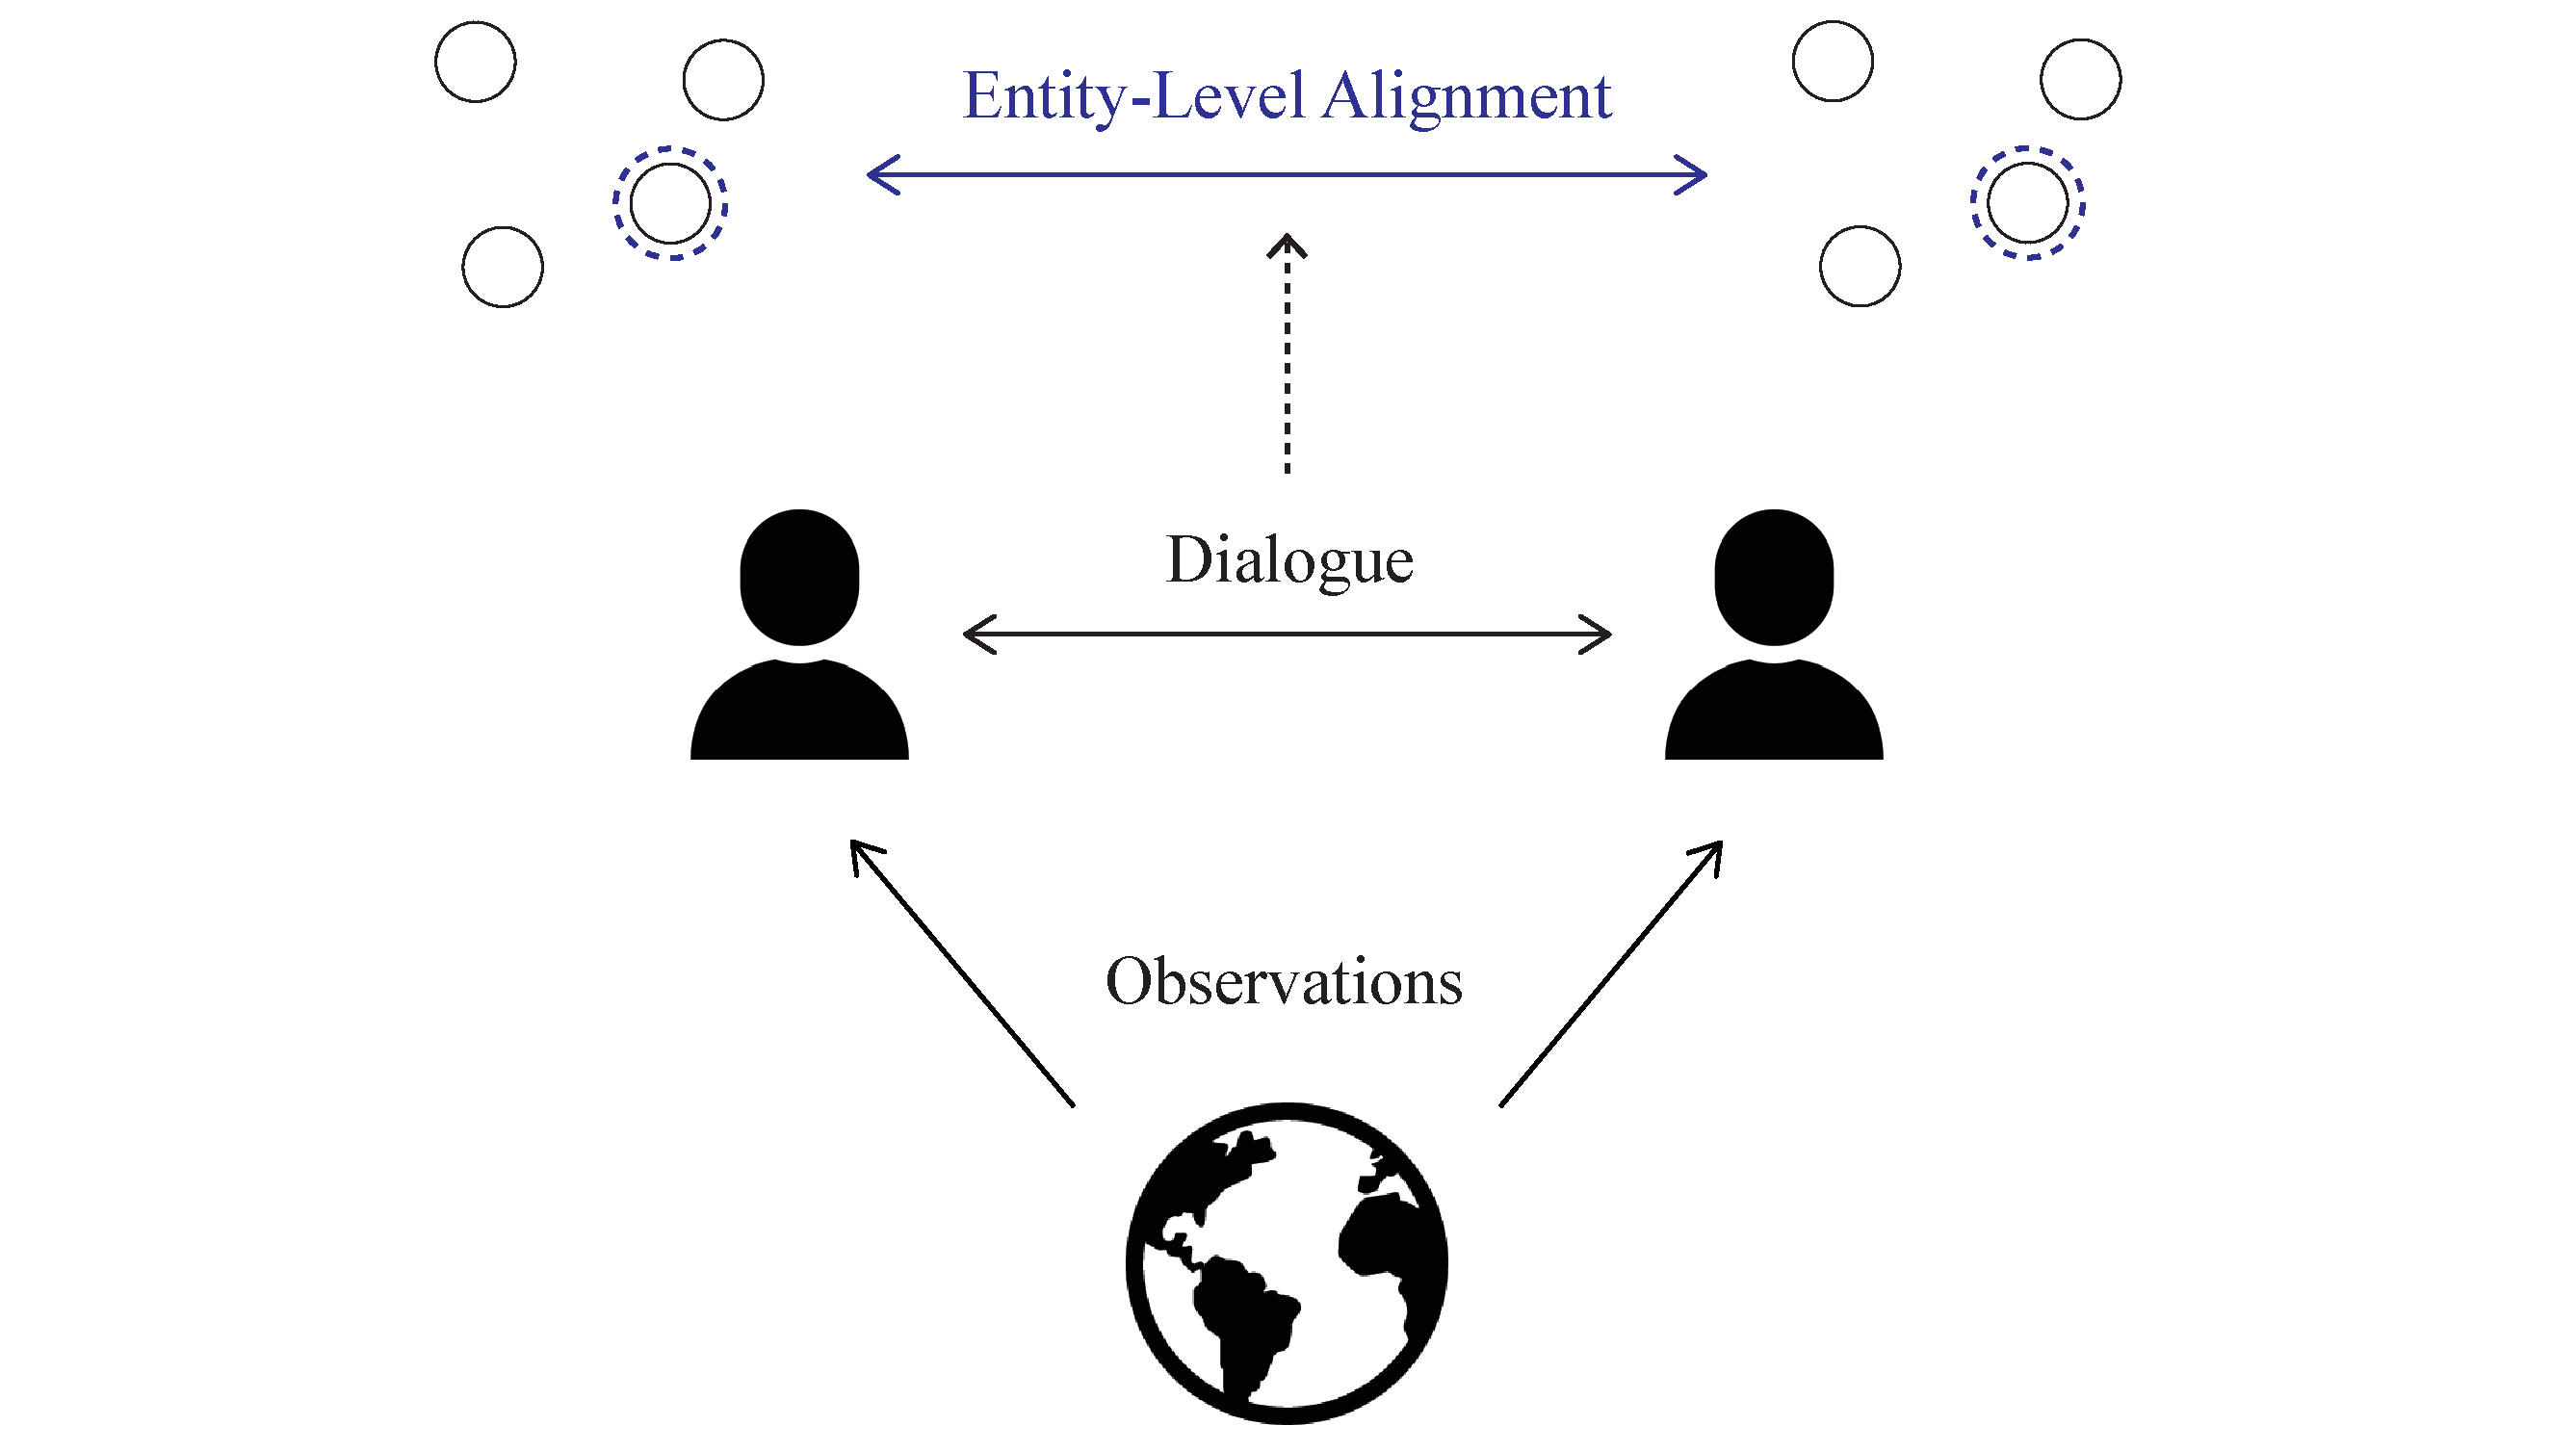
\includegraphics[width=\textwidth]{entity_level_alignment.pdf}
\caption{An illustration of our task formulation as \textit{entity-level alignment}.
}
\label{01_fig:entity_level_alignment}
\end{figure*}

To address all of these problems, we propose a novel research platform to study advanced common grounding in natural language dialogue systems. To make the scope of this thesis precise, we focus on the aspect of \textit{entity-level alignment} as the critical first step in general common grounding. As visually depicted in Figure \ref{01_fig:entity_level_alignment}, this step can be formalized as the following dialogue process:

\begin{enumerate}
  \item First, we assume that each speaker has a private \textit{observation} of the environment. This can be respresented as a personal experience, knowledge, perception, etc, typically involving multiple entities in the environment.

  \item Secondly, the speakers converse in natural language to recognize the same entity in the environent. The type of entity to be recognized can vary depending on the objective, e.g. physical objects, locations, or temporal events. 

  \item Finally, we consider common grounding to be \textit{successful} if and only if the speakers could recognize the same entity. In other words, we consider common grounding to be an accurate \textit{alignment} of the private observations at the \textit{entity-level}.
\end{enumerate}

For instance, the example dialogue \ref{ex_1:deictic_reference} can be considered as the alignment of a \textit{locational} entity and example \ref{ex_2:event_reference} as the alignment of an \textit{event} (or possibly its \textit{cause}). While this formalization is simplified and ignores the aspect of entire common grounding, entity-level alignment is a critical and indispensable step in any type of common grounding, e.g. developing common ground of an entire scenery \citep{das2017visual,haber-etal-2019-photobook,alamri2019audio}.

By restricting our scope to this preliminary setting, we address each of the three major limitations in the following ways.

\subsubsection{Contribution on the Task Settings}

\begin{figure*}[t!]
\centering
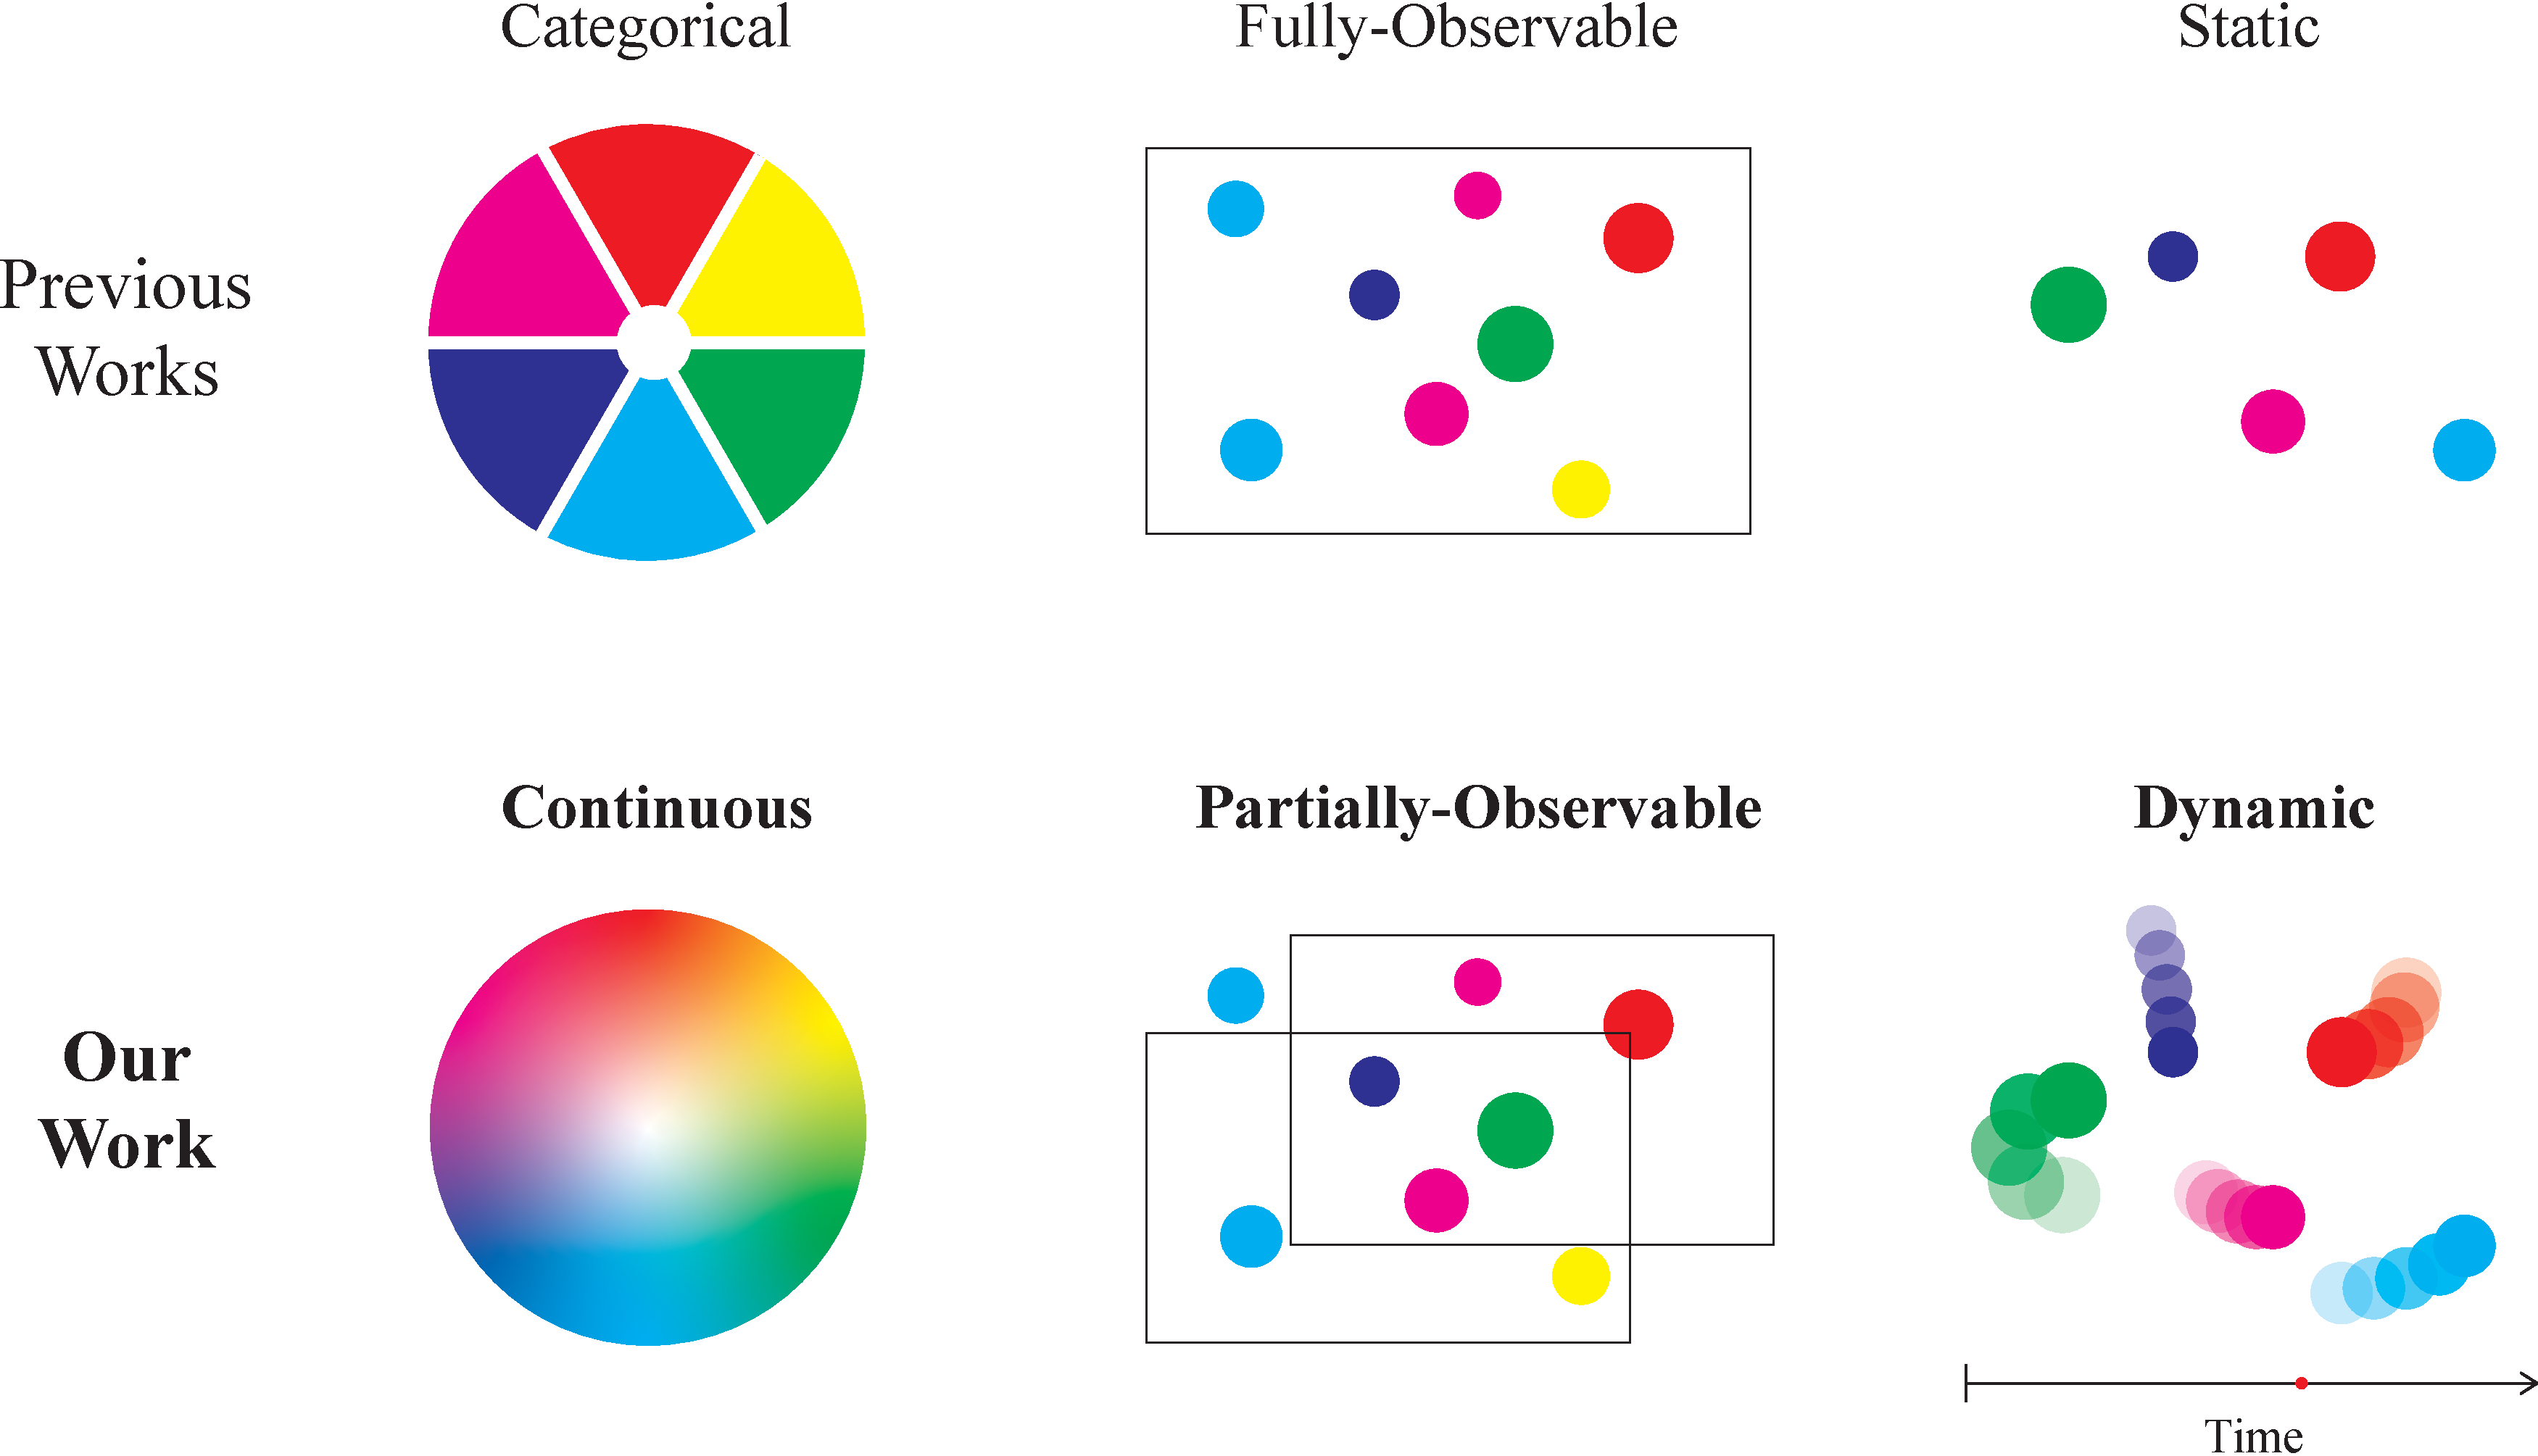
\includegraphics[width=\textwidth]{task_design.pdf}
\caption{An illustration of the task settings in previous works (top row) and our work (bottom row). We introduce \textit{continuity} to require more semantic coordination, \textit{partial observability} to require the resolution of potential misunderstandings, and \textit{dynamics} to incorporate the aspect of maintaining/updating common ground.
}
\label{01_fig:task_design}
\end{figure*}

We propose a novel task setting under \textit{continuous}, \textit{partially-observable} and (optionally) \textit{dynamic} context to require advanced skills of common grounding: see Figure \ref{01_fig:task_design} for a visual illustration in comparison to the previous settings. To be specific, we represent the dialogue context based on \textit{continuous} real values, which reflects the information (e.g. perception) in the physical world more faithfully and requires more advanced coordination, e.g. based on nuanced expressions \citep{paradis_2008} and pragmatic reasoning \citep{monroe2017colors}. In addition, we introduce \textit{partial-observability} where the agents have different perspectives of the environment, which is more realistic and requires to take into account the possibility of various misunderstandings \citep{keysar2000taking}. Finally (as an optional setting), we incorporate diverse \textit{dynamics} of the environments to require advanced skills of maintaining common ground: concretely, we incorporate dynamic scenes based on animations to require spatio-temporal reasoning \citep{girdhar2020cater} as well as information updates to require adaptation to the changing environments \citep{moon-etal-2020-situated}.

It is worth noting that each of these settings has been explored at least partially or independently in the previous literature: for instance, \citet{de2017guesswhat} proposed a reference game under \textit{continuous} visual context, and \citet{he2017learning} worked on a \textit{partially-observable} setting. However, our important contributions are the \textit{abstraction} of the task settings in the three universal dimensions and their \textit{combinations} to require more advanced common grounding. Owing to this level of abstraction, we can empirically investigate the consequences of each task setting in a scientific manner (i.e. through controlled experiments and hypothesis testing) and expect our findings to be general and fundamental for designing experimental setups in future dialogue research.


\subsubsection{Contribution on the Evaluation and Analysis}

\begin{figure*}[t!]
\centering
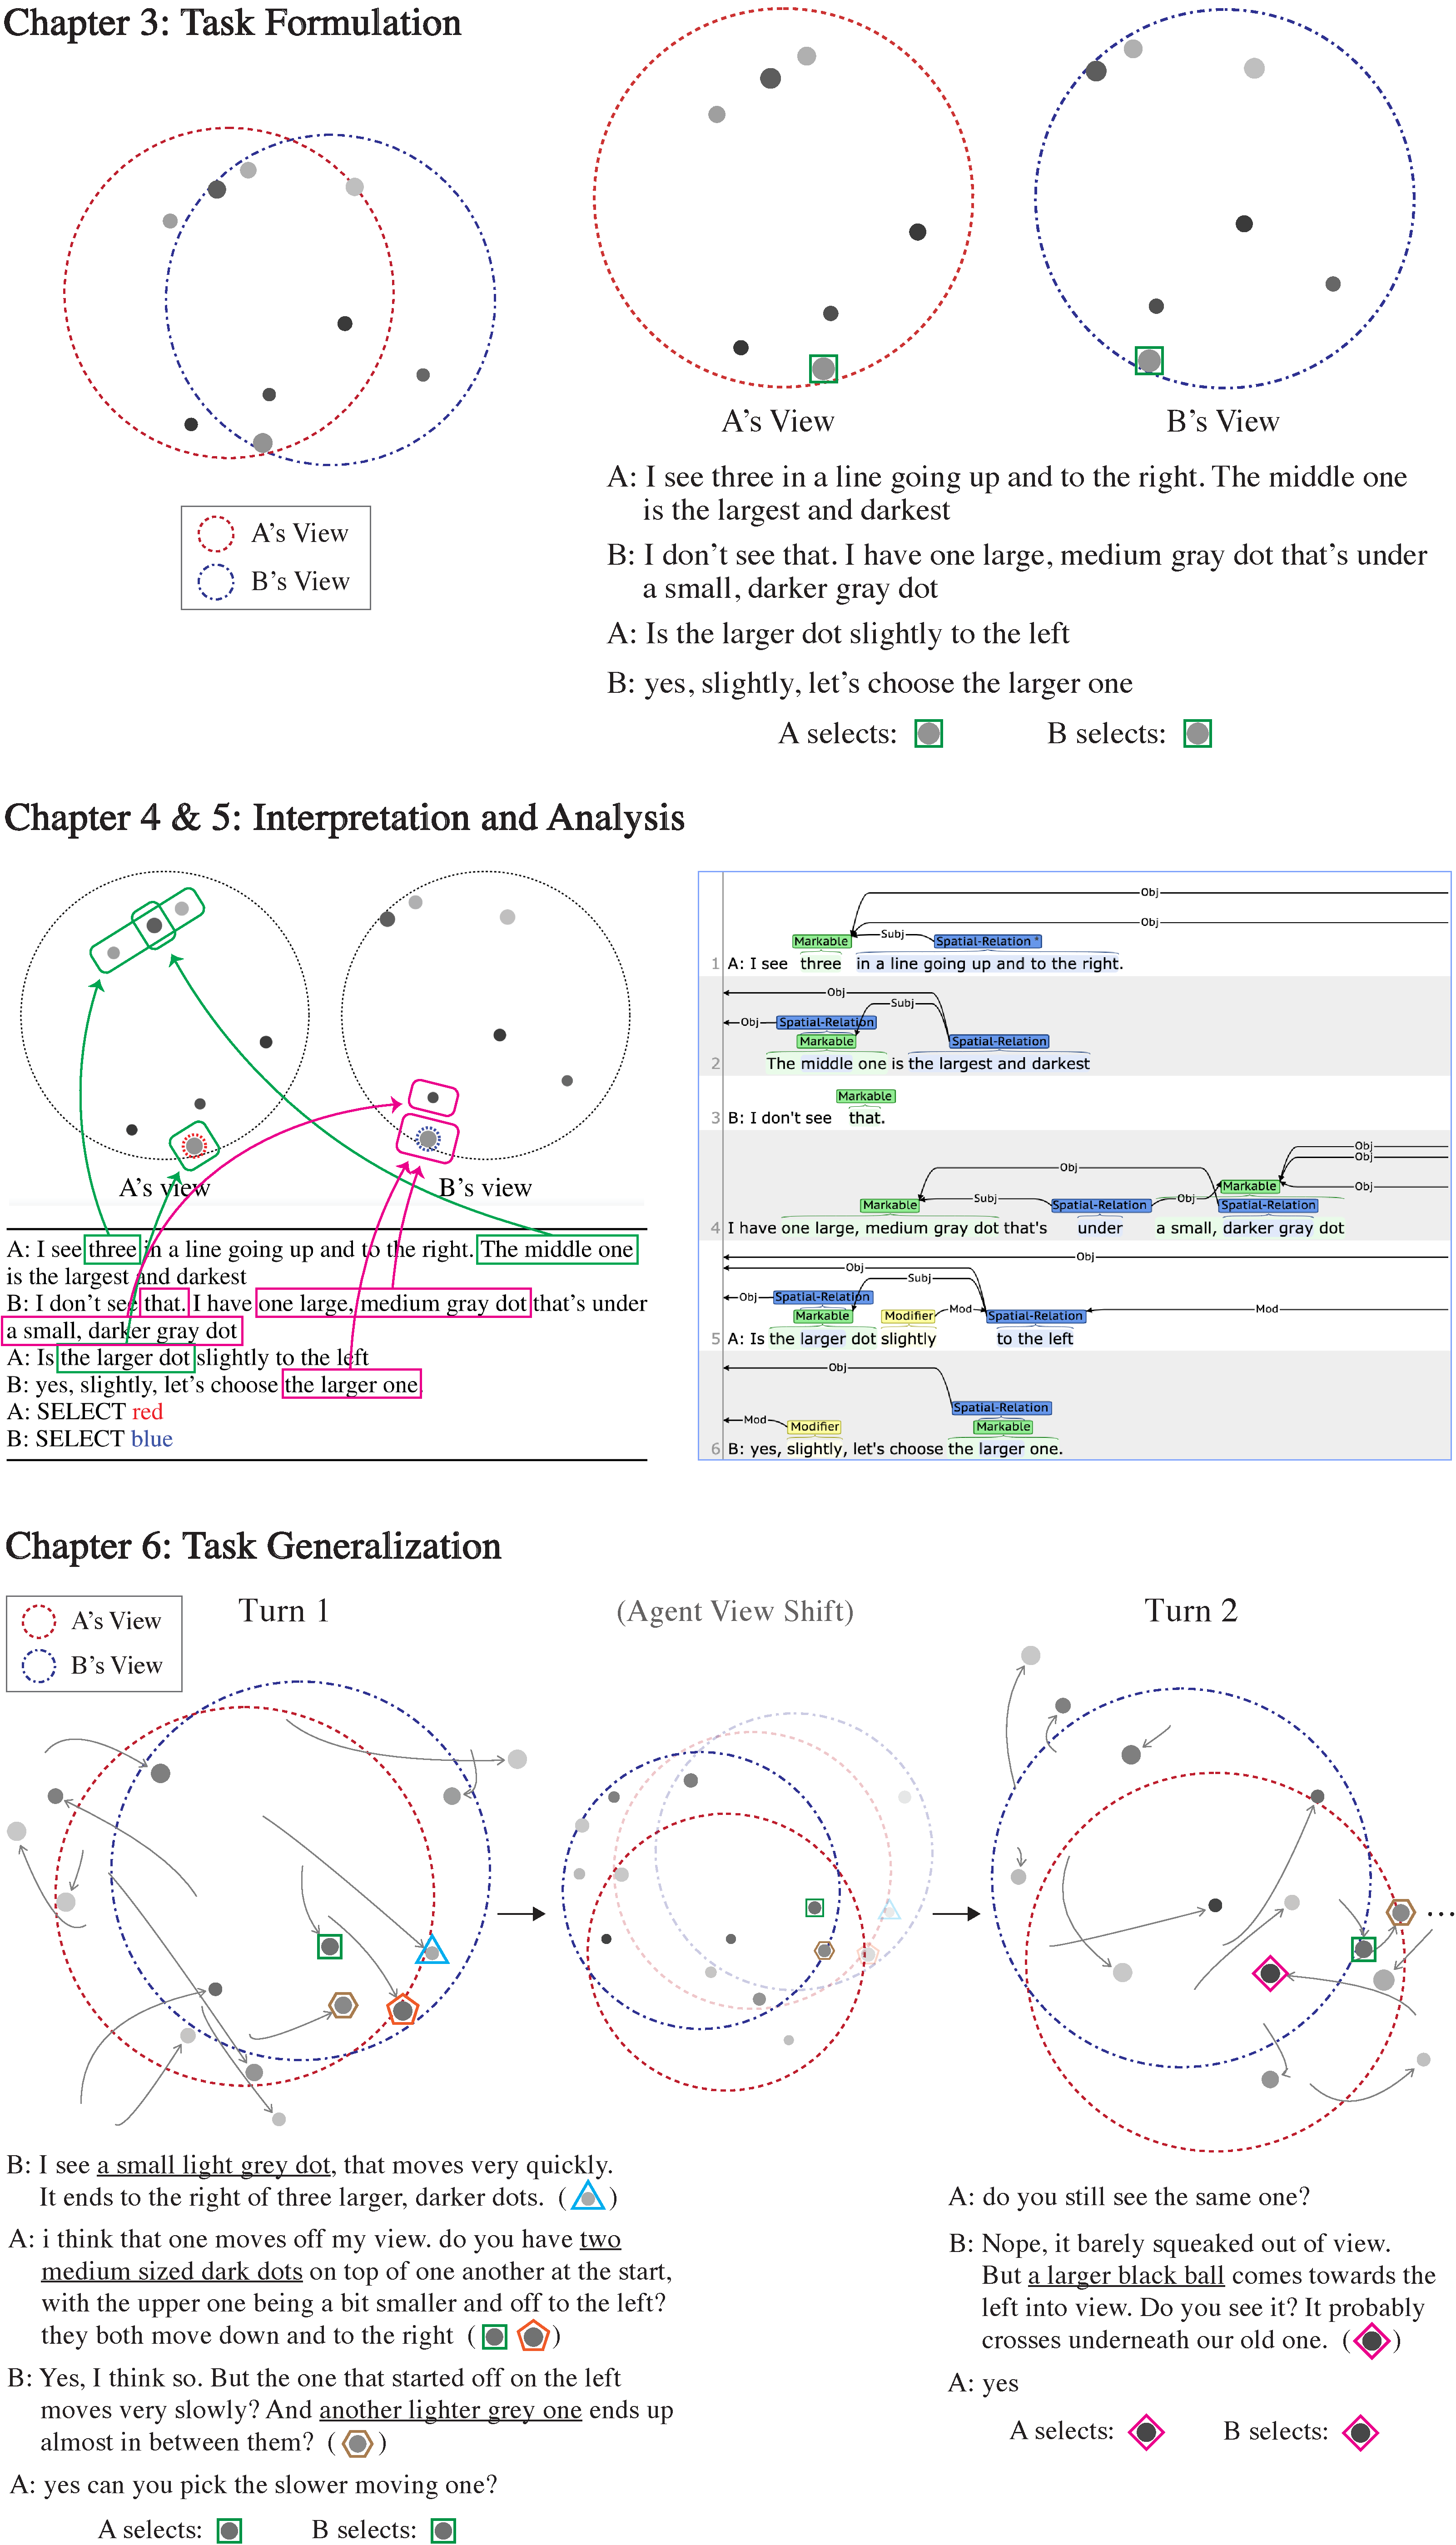
\includegraphics[width=\textwidth]{contribution_overview.pdf}
\caption{An overview of our task formulations and analytical frameworks.}
\label{01_fig:contribution_overview}
\end{figure*}

To evaluate the ability of creating common ground, we formulate a novel \textit{collaborative reference task}, where the goal of the agents is to select (i.e. coordinate attention on) the same entity through natural language dialogue. We consider this as an important step in general common grounding, since the mutual recognition of discourse entities (i.e. \textit{entity-level alignment}) is a fundamental building block in successful communication. Under this task formulation, we can evaluate the ability of accurate common grounding based on the \textit{task success rate}, which is both quantitative and objective. We also focus on a \textit{synthetic} environment to control, balance and diversify the dialogue contexts: this way, we can minimize undesirable biases and enable more faithful evaluation \citep{johnson2017clevr,girdhar2020cater}. We show an example dialogue of our collaborative reference task under \textit{continuous} and \textit{partially-observable} (but not \textit{dynamic}) context in Figure \ref{01_fig:contribution_overview} (top), which will be formally introduced in Chapter \ref{03_chp:task_formulation}.\footnote{Note that we also kept the \textit{task complexity} minimal for the ease of analysis.}

To analyze the process of common grounding, we propose a simple, reliable and useful framework of linguistic annotations. Specifically, we first identify the \textit{referring expressions} in the dialogue and the corresponding \textit{referent entities}, which can be in another modality (such as vision). This allows us to interpret the intermediate process of common grounding, such as how misunderstandings are introduced and resolved. Secondly, we conduct additional annotations to capture the detailed strategies of common grounding, such as how referring expressions are predicated or omitted in ellipses. To this end, we focus on \textit{spatial expressions} which are prevalent in visually grounded dialogues (including our own). We show an illustration of our analytical framework in Figure \ref{01_fig:contribution_overview} (middle), which will be discussed in detail in Chapter \ref{04_chp:interpretation} and \ref{05_chp:analysis}. Note that our analyses span different modalities (language and vision), which allow for investigating the related and important problem of \textit{symbol grounding} (c.f. Section \ref{02_sec:symbol_grounding}).

Under dynamic context, the collaborative reference task can be temporarily generalized to track and select the same entity at \textit{multiple timesteps} in the same environment: we refer to this as the \textit{sequential} collaborative reference task. Under this task formulation, we can further evaluate the ability of \textit{maintaining} accurate common ground based on the length of successful timesteps. We show an example dialogue of our sequential collaborative reference task in Figure \ref{01_fig:contribution_overview} (bottom), which will be formally introduced in Chapter \ref{06_chp:task_generalization}.

Based on the proposed task formulations and analytical frameworks, we enable reliable evaluation and detailed analysis of the fundamental aspects of common grounding.

\subsubsection{Contribution on the Model Capability}

Following the above ideas, we developed a collection of large-scale resources to train, evaluate and analyze various dialogue systems in terms of advanced common grounding. To be specific:

\begin{itemize}
  \item First, we collected 6,760 dialogues based on our minimal collaborative reference task under \textit{continuous} and \textit{partially-observable} context (Figure \ref{01_fig:contribution_overview}, top): we refer to this as OneCommon Corpus. Based on this dataset, we evaluate our baseline model's capability of \textit{recognizing} the created common ground in Chapter \ref{03_chp:task_formulation}.

  \item Secondly, we curated 5,191 successful dialogues from OneCommon Corpus and conducted the annotation of reference resolution (Figure \ref{01_fig:contribution_overview}, middle left). We describe how this resource can be leveraged to interpret and improve the common grounding strategies of our baseline model in Chapter \ref{04_chp:interpretation}.

  \item Thirdly, we randomly sampled 600 dialogues (already annotated with reference resolution) and further conducted the annotation of spatial expressions (Figure \ref{01_fig:contribution_overview}, middle right). Based on this annotation, we assess how well our improved baseline can recognize the fine-grained linguistic structures of the visually-grounded dialogues in Chapter \ref{05_chp:analysis}.

  \item Finally, we collected additional 5,617 dialogues based on our sequential collaborative reference task under \textit{continuous}, \textit{partially-observable} and \textit{dynamic} context (Figure \ref{01_fig:contribution_overview}, bottom): we refer to this as Dynamic-OneCommon Corpus. Based on this dataset, we assess our baseline model's capability of creating, retaining and updating common ground in dynamic environments in Chapter \ref{06_chp:task_generalization}.
\end{itemize}

In this thesis, we mainly focus on the simple and widely used \textit{end-to-end} dialogue systems \citep{vinyals2015neural,bordes2017learning,lewis-etal-2017-deal} as our baselines. However, our platform can be leveraged to experiment with various other approaches, as we discuss in Section \ref{02_sec:dialogue_systems}. While we leave further model assessments and improvements as future work, we propose a fundamental testbed for evaluating, analyzing and improving dialogue systems in terms of advanced common grounding.
\\

To summarize our contributions, we proposed novel task settings to study advanced common grounding as entity-level alignment. Based on our careful task designs, we formulated the (sequential) collaborative reference tasks to evaluate the ability of creating and maintaining accurate common ground. We also proposed useful analytical frameworks to interpret and analyze the intermediate process of common grounding. Finally, we developed large-scale resources for conducting various empirical studies, including the evaluation, analyses and improvements of data-driven dialogue systems.

Overall, we expect our proposed platform to be fundamental for promoting research on advanced common grounding in natural language dialogue systems.


\section{Thesis Outline}
\label{01_sec:thesis_outline}

The outline of this thesis is as follows:

\begin{itemize}
  \item In Chapter \ref{02_chp:literature_review}, we give an overview of the existing literature related to common grounding. This includes its theoretical foundations, computational research, and relationship with symbol grounding approached within various fields. Whenever appropriate, we clarify/explicate the novelty, motivations and contributions of this thesis to place them in these broader contexts.

  \item In Chapter \ref{03_chp:task_formulation}, we introduce a novel collaborative reference task under \textit{continuous} and \textit{partially-observable context}. Based on this task formulation, we collected 6,760 dialogues through crowdsourcing, which we refer to as OneCommon Corpus. Through our dataset analysis and experiment, we verified the advanced common grounding strategies required in this setting as well as the open room left for improvement. This chapter is based on our published work \citep{udagawa2019natural}.

  \item In Chapter \ref{04_chp:interpretation}, we propose a method of interpreting common grounding based on \textit{reference resolution}. Based on our novel framework, we annotated 5,191 dialogues from OneCommon Corpus via a combination of expert annotators and crowd workers. Our dataset analysis and experiment demonstrate the advantages of our annotation for interpreting the intermediate process of common grounding. This chapter is based on our published work \citep{udagawa2020annotated}.

  \item In Chapter \ref{05_chp:analysis}, we conduct further analyses by leveraging the existing annotation (reference resolution) to annotate \textit{spatial expressions}. We capture fine-grained linguistic structures of 600 dialogues in OneCommon Corpus, including predicate-argument structure, modification and ellipsis. Based on our improved baseline, we run a comprehensive assessment of the model's capability for recognizing such structures. This chapter is based on our published work \citep{udagawa-etal-2020-linguistic}.

  \item In Chapter \ref{06_chp:task_generalization}, we propose a novel task setting under \textit{dynamic} context to study the ability of mainining common ground. Based on our \textit{sequential} collaborative reference task, we crowdsourced 5,617 human dialogues, which we refer to as Dynamic-OneCommon Corpus. Through our dataset analysis and experiment, we demonstrate even more sophisticated strategies required in this setting in comparison to the \textit{static} counterpart of OneCommon Corpus. This chapter is based on our work to be published \citep{udagawa2021maintaining}.

  \item In Chapter \ref{07_chp:discussion}, we discuss the promising directions worth exploring in future research. Specifically, we propose further ideas on the \textit{task design methodologies} to require fully advanced common grounding, \textit{model improvements} to achieve more flexible and robust common grounding, and \textit{real-world applications} that naturally follow from the studies in this thesis.
\end{itemize}



\graphicspath{{02_literature_review/figures/}} % Location of the graphics files

\chapter{Literature Review}
\label{02_chp:literature_review}

Due to the foundational aspect of common grounding, there is a rich and diverse literature related to this topic. In this chapter, we first give an overview of the existing literature on common grounding (Section \ref{02_sec:common_grounding}). Then, we review the contemporary approaches to dialogue system engineering (Section \ref{02_sec:dialogue_systems}). Finally, we discuss the important links to the related (yet distinct) problem of symbol grounding (Section \ref{02_sec:symbol_grounding}).

\section{Common Grounding}
\label{02_sec:common_grounding}

In this section, we first give an overview of the theoretical foundations of common grounding, including the literature in philosophy, mathematical logic and psycholinguistics (Section \ref{02_subsec:theoretical_foundations}). Then, we review the computational models of common grounding in natural language conversations, including both formal and empirical approaches (Section \ref{02_subsec:computational_approaches}).

\subsection{Theoretical Foundations}
\label{02_subsec:theoretical_foundations}

The notion of common ground (or \textit{common knowledge}) was originally conceived by David Lewis \citep{lewis1969convention} to explain the nature of human \textit{conventions}. Conventions are the regularities in our behavior which we expect each of us to understand and follow: without them, we cannot account for our solutions to various \textit{coordination problems} \citep{Schelling1960}, from setting up daily meetings to communicating in natural language. In essence, \citeauthor{lewis1969convention} argues that such expectations can only be justified based on a certain level of common ground established within the community.

In later studies, common ground came to be recognized as ubiquitous and essential in various linguistic phenomena/competence, including presupposition \citep{stalnaker1978assertion}, definite reference \citep{Clark1981-CLADKA}, communication \citep{clark1996using} as well as first language acquisition \citep{clark2001grounding}.

But what exactly is common ground? Can it be defined formally, and do we know how exactly they are built up? The absolute answers may not be established yet, but there are three major approaches which account for these questions.\\

\noindent
\textbf{Epistemic Logic}\quad
The first approach is studied in the field of epistemic modal logic \citep{fagin2003reasoning}. To give a brief introduction, we consider $A$ to be the set of agents and $p$ to be a proposition. Then, using the modal operator $K_a$, we can represent the epsitemic state that ``an agent $a \in A$ knows $p$'' as $K_a\,p$. Similarly, we can represent the state that ``all agents in $A$ know $p$'' based on the operator $E_{A}\,p$ (which is equivalent to $\bigwedge_{a \in A} K_a\,p$). Finally, if we use the abbreviation $E_{A}^n\,p$ for $E_{A}\,E_{A}^{n-1}\,p$ (where $E_{A}^{0}\,p\,=\,p$), we can represent the state ``$p$ is \textit{common knowledge} among $A$'' based on the operator $C_{A}\,p$ (which is equivalent to $\bigwedge_{i=1}^{\infty} E_{A}^i\,p$).

The process of common grounding can be taken into account by using additional operators which represent the \textit{actions} or \textit{events} that cause the change in agents' epistemic states: such logical framework is known as dynamic epistemic logic \citep{van2007dynamic}. If we assume the agents to be perfectly logical reasoners, this framework allows for computing the exact set of common ground after each information update.

However, the formulations and assumptions in this approach may not be cognitively plausible. For instance, a literal interpretation of common knowledge imposes an infinite list of epistemic conditions to be checked \citep{Clark1981-CLADKA}, and humans may not be perfect logical reasoners either. This drawback makes the theory difficult to be applied in realistic settings, such as natural language dialogues.
\\

\noindent
\textbf{Shared Basis}\quad
The second approach defines common ground based on the notion of \textit{shared basis} \citep{lewis1969convention,Clark1981-CLADKA}. To be specific, this approach considers a proposition $p$ to be common ground among the agents i.f.f. there exists some state of affairs $b$ such that:

\begin{enumerate}
  \item Every agent has information of the basis $b$.
  \item $b$ indicates to every agent that every agent has information of $b$.
  \item $b$ indicates to every agent that $p$ holds.
\end{enumerate}

For instance, in a situation where agents are \textit{co-present} and \textit{co-observing} a house on fire, these state of affairs become the shared basis for the common ground ``there exists a house on fire''. This approach is more cognitively plausible because the infinite, recursive assessment of epistemic states is not required (as in the previous approach). Furthermore, the shared basis need not be represented symbolically and hence accounts for \textit{multi-modal} (non-linguistic) common grounding through gestures \citep{lascarides2009formal}, eye gaze \citep{nakano-etal-2003-towards} and other mediums that are commonly used in face-to-face interactions.

However, current approaches so far define common ground independently for each proposition $p$. Is it possible to define common ground (and common grounding) in its entirety, including their interrelationships and non-propositional knowledge? The last approach offers an interesting perspective which takes this into account.
\\

\noindent
\textbf{Situation Models}\quad
The last approach employs the concept of \textit{situation models}. Situation models are the mental representations of the state of affairs described in text or conversation \citep{zwaan1998situation}. For instance, there is empirical evidence in cognitive psychology that humans are sensitive to spatial layouts when comprehending stories \citep{GLENBERG198769} and constructs spatially coherent representations as they read along \citep{ferguson1994properties}. These studies suggest that comprehension of language is not merely an analysis of syntactic/semantic structures, but should rather be considered as construction of situation models coherent with the linguistic descriptions (e.g. in terms of spatial, temporal and causal dimensions).

Following this idea, \citet{pickering2004toward} consider common ground(ing) as the \textit{alignment} of situation models among the interlocutors. Based on this view, the process of common grounding does not require explicit reasoning of the epistemic states, as required in the previous approaches. Instead, they argue that such alignment proceeds mostly implicitly at various linguistic levels, including phonetic, lexical, syntactic and semantic representations. For instance, lexical entrainment naturally leads to aligned conceptualization, which is also in line with the theory of \textit{conceptual pacts} \citep{Brennan1996ConceptualPA}.

This approach has the advantage of representing the entire common ground as the \textit{aligned situation models}, which capture the holistic view of common ground (including their internal structures and non-linguistic knowledge). However, the lack of strict definitions and strong empirical evidence (e.g. on how situation models are actually aligned) potentially remain as its major challenges.\\

It is worth noting that our formalization of common grounding (Section \ref{01_sec:contributions}) is closest to the last definition by \citet{pickering2004toward}. However, we circumvent the difficulty of dealing with entire situation models by restricting our scope to \textit{entity-level alignment}, which keeps the task simple, well-defined and quantifiable.

\subsection{Computational Approaches}
\label{02_subsec:computational_approaches}

The previous section focused on the conceptual (\textit{epistemic logic}) or psychological (\textit{shared basis} and \textit{situation models}) foundations of common grounding. Unfortunately, they are not directly applicable for our practical goal of developing \textit{computational} models of common grounding through \textit{natural language} interaction.

\subsubsection{Formal Approaches}

To model common grounding in actual human conversations, \citet{traum1994computational} conducted a pioneering work based on a refinement of the contribution theory \citep{clark1989contributing}. To be specific, he defined a set of \textit{grounding acts} (such as \textit{initiate}, \textit{continue}, \textit{repair}, \textit{request repair} and \textit{acknowledge}) by taking into account the speech acts \citep{austin1962things,searle1969speech} relevant to common grounding. Based on these grounding acts, a finite state model is used to compute the transition of information in dialogue, until it reaches the final accepting state (and considered to be in common ground).

In subsequent works, the idea of this approach has been integrated with Discourse Representation Theory \citep{Kamp1981-KAMATO-2,kampreyle93} to represent the semantic (e.g. propositional) contents of common ground \citep{poesio1997conversational}. In Segmented Discourse Representation Theory \citep{asher2003logics}, \textit{rhetorical relations} are also taken into account to capture the implicit process of common grounding, e.g. through the initiation of the next relevant contribution. Such formal representations provide elaborate computational models of not only common grounding but natural language dialogue in general \citep{ginzburg2012interactive}.

However, formal approaches come with their own disadvantages. For instance, identifying the precise semantic representation of a dialogue is a challenging task requiring time and high expertise. They are also unable to capture various complexities in realistic dialogues, such as ambiguity and uncertainty in common grounding. Finally, they are not directly applicable to \textit{situated} dialogues involving rich non-linguistic contexts, such as vision and embodied environments.

\subsubsection{Empirical Approaches}

To overcome these limitations, recent works mostly focus on empirical methods and develop \textit{data-driven} models of common grounding. The primary step in this approach is to collect dialogue corpora: such attempts have originated in the HCRC Map Task Corpus \citep{anderson1991hcrc} and continued since then \citep{potts2012goal,tokunaga-etal-2012-rex,zarriess-etal-2016-pentoref}. Recent works often utilize crowdsourcing to collect diverse data at scale: notable works include the GuessWhat?! dataset \citep{de2017guesswhat}, MutualFriends dataset \citep{he2017learning}, PhotoBook dataset \citep{haber-etal-2019-photobook} as well as our own \citep{udagawa2019natural,udagawa2021maintaining}. As an illustration, we show an excerpt of the common grounding task from the PhotoBook dataset in Figure \ref{02_fig:photobook_sample}, where the human players try to identify the common images through dialogue.\footnote{Note that the players are indeed relying on \textit{entity-level alignment} to succeed in common grounding.}

\begin{figure*}[t!]
\centering
\includegraphics[width=\textwidth]{photobook_dataset_sample.pdf}
\caption{An excerpt from the PhotoBook dataset \citep{haber-etal-2019-photobook}. In this task, two human players are provided different combinations of images and try to find out whether the (bordered) images are in common or not.
}
\label{02_fig:photobook_sample}
\end{figure*}

The second step is employ machine learning \citep{murphy2012machine} to train the models based on the collected corpora, typically in an \textit{end-to-end} or fully data-driven manner. By leveraging the actual human dialogues, we can expect the models to learn fundamental strategies of common grounding (e.g. clarifications and elaborations) without expensive, potentially unreliable annotations. We can also expect the models to capture the ambiguity and uncertainty in common grounding owing to their high flexibility. Finally, this approach can naturally be applied in situated conversations, e.g. by treating multi-modal information in a unified manner based on neural networks \citep{GoodBengCour16}. We will explain the specific model architectures in Section \ref{02_subsec:models}.

Note that most of the existing common grounding tasks focus on closed domain, goal-oriented dialogues, including our collaborative reference tasks (c.f. Figure \ref{01_fig:contribution_overview}): this is for the sake of quantitative and objective evaluation based on the \textit{task success rates}, as we discussed in Chapter \ref{01_chp:introduction}. However, some recent works also attempt to model this in open domain, non-goal-oriented dialogues: for instance, \citet{cho-may-2020-grounding} developed a model of (single-turn) common grounding through creative improvisation of the next relevant contribution. While its evaluation remains an open challenge, this new approach sheds light on interesting potential applications, such as the development of more engaging, entertaining and coherent chat-bots.

\section{Dialogue Systems}
\label{02_sec:dialogue_systems}

In this section, we review the broader literature of dialogue system research in general. Unfortunately, most of the existing works do not specifically focus on common grounding: for instance, they do not require advanced common grounding skills nor enable direct evaluation/analysis of such abilities. However, understanding the broader literature is fundamental for common grounding research, since they provide crucial insights on the related problems and engineering solutions. Besides, it is important to place the role of common grounding in the general settings of dialogue, which will be one of the main focuses of this section.

\subsection{Tasks and Datasets}
\label{02_subsec:tasks_and_datasets}

Dialogue research is conducted under various motivations and practical goals: consequently, numerous tasks and datasets have been proposed in the existing literature. To make our review as inclusive as possible, we categorize them into the following 4 types: namely \textit{(traditional) task-oriented dialogues}, \textit{multi-modal dialogues}, \textit{non-cooperative dialogues}, and \textit{non-goal-oriented dialogues}.
\\

\noindent
\textbf{Task-Oriented Dialogues}\quad
Traditionally, the central motivation of dialogue system research has been a practical one: to develop industrial-level dialogue systems that can execute a variety of useful tasks. The expected tasks include booking a trip \citep{elasri2017frames} or recommending movies \citep{chen-etal-2019-towards} by interactively soliciting the user's preferences. Due to its practicality, many existing benchmarks and shared tasks have been focusing on such task-oriented dialogues \citep{henderson-etal-2014-second,budzianowski-etal-2018-multiwoz,lee2019multi}. Recent works propose valuable extensions as well, e.g. based on scalable task ontologies \citep{rastogi2020towards} and efficient domain adaptations \citep{shalyminov2020fast}

However, the underlying settings in these tasks remain mostly unchanged and do not require advanced common grounding. To be specific, they only need to deal with \textit{categorical} databases or knowledge graphs, which do not require semantic coordination from the ground up. For instance, continuous concepts like the price range would be discretized in advance (e.g. to ``cheap'', ``moderate'' and ``expensive''), so that they can avoid sophisticated common grounding and keep the tasks manageable. 

If we were to develop truly conversational and practical systems, we should start focusing on systems that can deal with more advanced settings, e.g. that can negotiate on the exact preferences on a \textit{continuous} scale. Without such ability, dialogue systems cannot adequately respond to the user's precise requests, e.g. in terms of the price range, location, atmosphere, and so on.\\

\noindent
\textbf{Multi-Modal Dialogues}\quad
Recently, increasing attention has been paid to multi-modal dialogues, especially those grounded in the visual modality \citep{das2017visual,de2017guesswhat,alamri2019audio}. These works lie at the intersection of computer vision (CV) and NLP, involving intricate cognitive reasoning \citep{zellers2019recognition} and spatio-temporal grounding (c.f. Section \ref{02_subsec:spatio_temporal_grounding}). Such extension to the visual modality is also useful in practice. For instance, \citet{moon-etal-2020-situated} proposed a dialogue task where the system can display and manipulate a shared screen with the user: this allows for better interaction and improved user experience, especially in shopping domains (e.g. for fashion and furniture) where item apperances play a key role.


However, it remains unclear to what extent existing tasks require precise dialogue understanding and spatio-temporal grounding. First, there are minimal linguistic analyses conducted on these datasets, and the complexities of the dialogue structures remain unrevealed. Secondly, there could be various sources of undesirable biases in realistic visual contexts \citep{goyal2017making,cirik-etal-2018-visual}, and the tasks may not necessarily require genuine intricate abilities. For instance, existing visual dialogue tasks may be largely solvable without taking into account \textit{dialogue history} \citep{agarwal-etal-2020-history}, contrary to the expectation when it was first proposed \citep{das2017visual}.

Therefore, we argue that more attention must be paid to the requisite skills of visually-grounded dialogues and their reliable evaluation. Common grounding and symbol grounding are the two central competence we focus on and address in this thesis.
\\

\noindent
\textbf{Non-Cooperative Dialogues}\quad
All of the previous tasks so far (including the common grounding tasks) have assumed that dialogue is \textit{cooperative}, i.e. the goals of the interlocutors are fully aligned. However, this may not necessarily be the case in general. Typical departures include the cases of negotiation \citep{lewis-etal-2017-deal,he-etal-2018-decoupling,li2020noncollaborative}, where the interlocutors' goals may be different or even conflicting (e.g. they must compete for a fixed amount of resource). Such situations may also arise when one needs to persuade the other to profit a third party \citep{wang-etal-2019-persuasion} or in the case of malicious scams where one is intending to deceive the other \citep{li2020noncollaborative}. On such occasions, the interlocutors need to exert complex reasoning skills and negotiation strategies to achieve their desired outcomes.

However, this does \textit{not} indicate that common grounding can be non-cooperative in such settings. On the contrary, we argue that fully cooperative common grounding plays a fundamental role in maintaining any type of conversation. Even in the case of negotiation, the interlocutors must cooperate and share (certain levels of) the same understandings to disagree, compromise, or take any extreme measures \citep{lewis1969convention,sacks1987preferences}. This suggests that we must take into account the collaborative aspect of common grounding, even if our goal was to study dialogues in non-cooperative settings.
\\


\noindent
\textbf{Non-Goal-Oriented Dialogues}\quad
Finally, we raise the category of \textit{non-goal-oriented} dialogues, typically referred to as chit-chats. The main objective of this research is to develop \textit{engaging} and \textit{coherent} chatbots that can handle a wide variety of topics, ranging from sports, politics to technology \citep{ram2018conversational}. One key factor that affects engagement is \textit{empathy}, the cognitive ability of understanding and acting on behalf of the user's emotional states. Microsoft XiaoIce, one of the world's most popular chatbots today, explicitly incorporates such empathetic mechanisms \citep{zhou2020design}. To assess and improve the consistency of chatbots, \citet{zhang-etal-2018-personalizing} proposed a dialogue setting where the interlocutors are provided artificial profiles to act in accordance to. In subsequent works, the profiles are extended to fictitious character settings and grounded in more open-ended text adventure games \citep{urbanek-etal-2019-learning}.

In recent years, there has been an impressive breakthrough on the model side based on gigantic-scale neural networks \citep{adiwardana2020towards,roller-etal-2021-recipes}. While they exhibit almost human-level performance under specific setups, they still do not possess the true competence of natural language conversation. To demonstrate this, \citet{benotti-blackburn-2021-grounding} raised an example dialogue with BlenderBot, the state-of-the-art chatbot from Facebook \citep{smith-etal-2020-put,roller-etal-2021-recipes}:

\ex.
\a. Human:\; Do you know Blender?
\b. BlenderBot:\; Yes, I've used it a little bit. I am not very good at it, though.
\c. Human:\; But I don't mean the 3D software.
\d. BlenderBot:\;  Oh, I see. Yeah, I know a little bit about it. What do you like to do with it?
\e. Human:\; I mean Blender, the chatbot. Have you used it?
\f. BlenderBot:\; Oh, yes, I have used it. I like to use it to make 3D models.

In this conversation, the human speaker clarifies that ``Blender'' refers to the chatbot and not the 3D software (c). Impressively, BlenderBot acknowledges its misunderstanding and makes a perfectly coherent recovery (d). However, in the last utterance (f), it turns out that BlenderBot had not actually resolved its misunderstanding and once again misinterprets ``Blender'' as the 3D software. 

This example demonstrates the lack of true common grounding capacity of modern chatbots: in this case, the ability of accurate \textit{entity-level alignment}. To realize truly engaging and coherent chatbots, we expect that more robust and reliable common grounding will be the key in non-goal-oriented dialogues as well.

\subsection{Evaluation Metrics}
\label{02_subsec:evaluation}

Evaluation plays a crucial role in the development of dialogue systems. The specific measures can vary depending on the task domain: for instance, the \textit{task success rate} may be the primary metric in task-oriented dialogues, \textit{each player's payoff} may be so in non-cooperative dialogues and \textit{user satisfaction} in non-goal-oriented dialogues. Such evaluation can be conducted either manually (e.g. based on questionnaires) or automatically (e.g. based on regressions from the relevant factors, \citealt{walker-etal-1997-paradise}).

There are also task agnostic approaches to dialogue evaluation. For instance, \textit{human-likeness} is usually a desirable factor in all types of dialogues. While this is relatively straightforward to measure manually based on human judgements, automatic evaluation of such quality remains an open challenge. For instance, reference-based metrics such as BLEU \citep{papineni-etal-2002-bleu} may not correlate with human evaluation \citep{liu2016}, and regression-based metrics such as ADEM \citep{lowe-etal-2017-towards} can easily be fooled by simple adversarial attacks \citep{sai2019re}.

For a comprehensive review of existing evaluation methodologies, we refer to a recent survey by \citet{Deriu2020SurveyOE}. However, throughout this thesis, we argue that the evaluation of dialogue systems should focus more on their \textit{abilities} \citep{Hernndez-Orallo:2017:MME:3110808} rather than the ad-hoc performance metrics (such as benchmark scores). This means that we should answer the following research questions through the design of dialogue tasks and evaluation metrics:

\begin{itemize}
	\item What are the specific abilities required to succeed in this task setting?
	\item Does the evaluation metric truly reflect such abilities?
\end{itemize}

In the field of psychometrics, these two questions roughly correspond to the concepts of \textit{validity} and \textit{reliability}, respectively \citep{cook2006current}. Unfortunately, current evaluation of dialogue systems often neglects the first question: for instance, it is not made clear what linguistic capabilities and strategies are required in a certain dialogue setting. Many works also fail to answer the second question: for instance, the existence of dataset biases makes the evaluation unreliable and unfaithful.

From this aspect, we hope this thesis contributes important insights on the requisite skills and evaluation of \textit{common grounding}, which should be taken into account in all types of dialogues (as discussed in Section \ref{02_subsec:tasks_and_datasets}).

\subsection{Model Architectures}
\label{02_subsec:models}

Finally, we give an overview of the mainstream architectures in dialogue system engineering. As briefly discussed in Chapter \ref{01_chp:introduction}, there are two major approaches in developing modern dialogue systems. In Figure \ref{02_fig:two_dialogue_systems}, we show an illustration of the two approaches from a recent survey paper \citep{gao2019neural}.\\

\begin{figure*}[th!]
\centering
\includegraphics[width=0.95\textwidth]{two-dialogue-system.pdf}
\caption{An illustration of the two mainstream architectures of data-driven dialogue systems from \citet{gao2019neural}.
}
\label{02_fig:two_dialogue_systems}
\end{figure*}

\noindent
\textbf{Traditional Dialogue Systems}\quad
The first approach is based on a pipeline/modular architecture, which has traditionally been used for task-oriented dialogue systems (Figure \ref{02_fig:two_dialogue_systems}, top). In this framework, the \textit{natural language understanding (NLU) module} is first applied to the user utterance to extract relevant information, typically in a structured format. This can be as simple as a pair of user intent and named entities \citep{Gupta2006TheAS} or more complex graph-based representations which capture anaphora, relations, and utterance ambiguity \citep{kollar-etal-2018-alexa}. Next, the \textit{dialogue state tracker} integrates the extracted information with the previous dialogue state to update the current state. Dialogue states are often represented based on the \textit{frame} structure (i.e. slot-value pairs), possibly one for each domain under control \citep{elasri2017frames}. In a recent approach, these are extended to executable data-flow graphs \citep{andreas-etal-2020-task} which are much more general and expressive. Based on the updated dialogue state, the system can optionally query the database for necessary information \citep{dhingra-etal-2017-towards} and the \textit{dialogue policy module} determines the content of the system response \citep{takanobu-etal-2019-guided}. Finally, the \textit{natural language generation (NLG) module} either retrieves an appropriate response template \citep{yan2016learning} or generates the surface form conditioned on the determined content \citep{wen-etal-2015-semantically}.\\

\noindent
\textbf{End-to-End Dialogue Systems}\quad
In the second approach, dialogue systems are typically trained in a fully data-driven manner based on \textit{end-to-end} neural networks. Under this setting, dialogue modeling is often treated as a type of \textit{(conditional) language modeling} problem \citep{vinyals2015neural}: conditioned on the input sequence of dialogue history, compute the probability of the next dialogue responses.

Formally, let $D = \{d^1, d^2, ..., d^{|D|}\}$ be the dialogue corpus containing the dialogue sequence $d^i = \{x^i_1, x^i_2, ..., x^i_{|d^i|}\}$. We generally consider each element of the dialogue sequence $x^i_t$ to be a \textit{token}: however, it can also be in the unit of the whole \textit{utterance} \citep{serban2016hierarchical}. Given $D$ as the dataset, the learning objective is to find the model parameters $\theta$ that minimize the sum of negative log probabilities (or equivalently, maximize the product of total probabilities)
%
\begin{equation}\label{eqt:sequence_to_sequence}
L(\theta) = \sum_{i = 1}^{|D|} \sum_{t = 1}^{|d^i|} - \log p(x^i_t | x^i_{<t}, \theta)
\end{equation}
%
where $x^i_{<t} = \{x^i_1, x^i_2, ..., x^i_{t-1}\}$ (which represent dialogue history).

\begin{figure*}[th!]
\centering
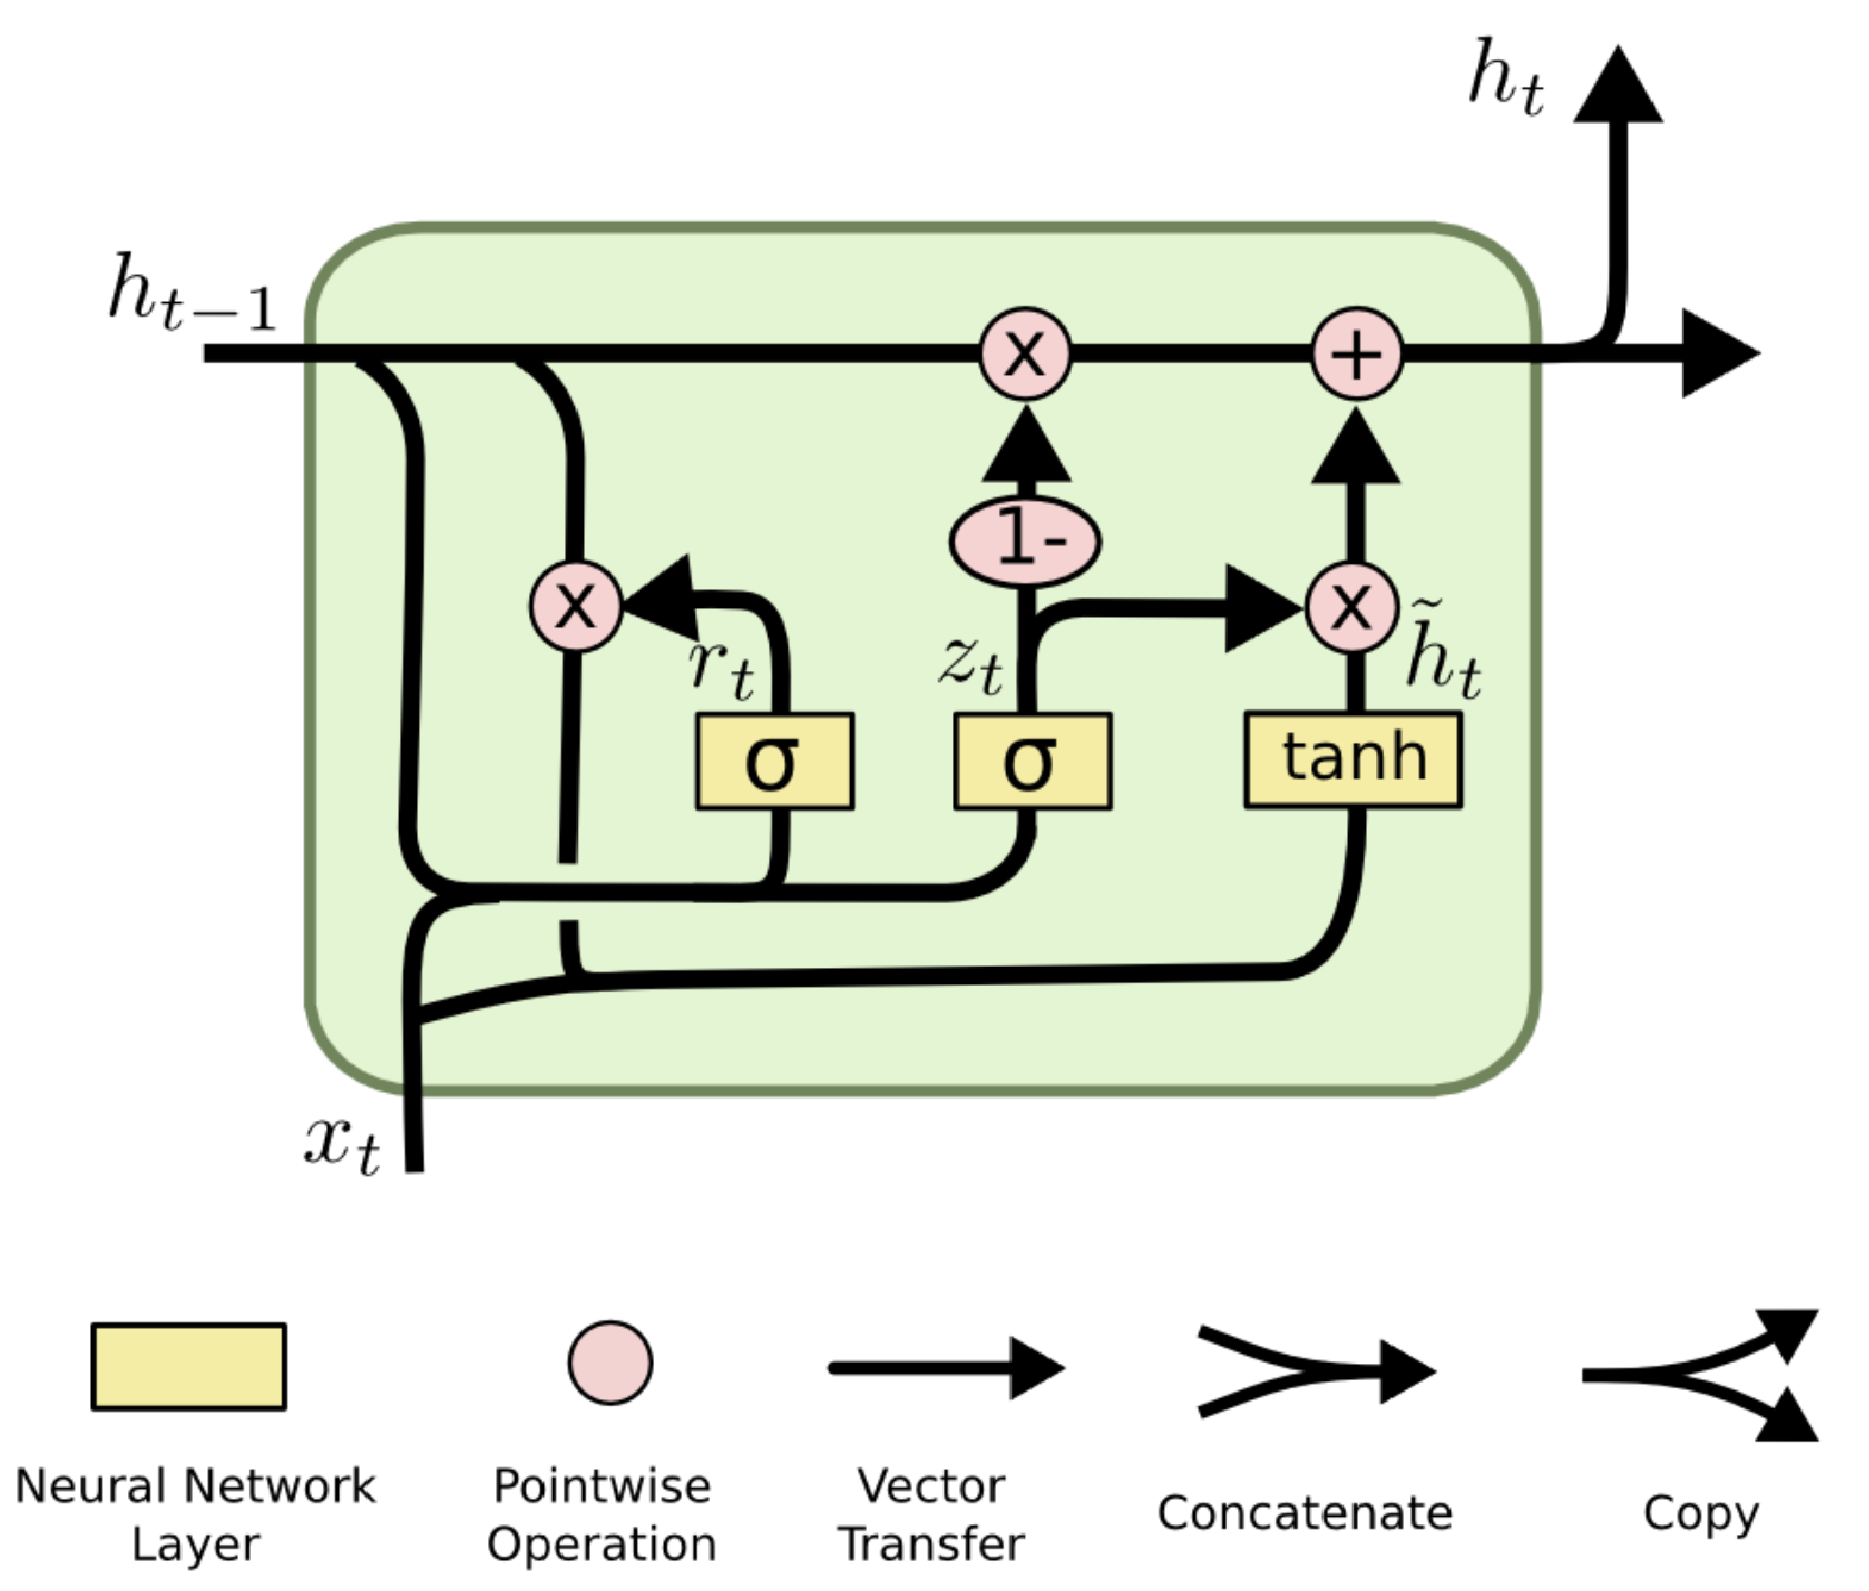
\includegraphics[width=0.6\textwidth]{gated_recurrent_unit.pdf}
\caption{An illustration of the Gated Recurrent Unit (GRU) architecture, from the online post by \citet{olah2015understanding}.}
\label{02_fig:gru_architecture}
\end{figure*}

This can be modeled by a variety of deep learning architectures in the \textit{encoder-decoder} framework. Specifically, we first encode the dialogue history $x^i_{<t}$ with an \textit{encoder}, followed by a \textit{decoder} to predict $x^i_{t}$. There are multiple architectures that can handle this, including LSTM \citep{hochreiter1997long}, GRU \citep{cho2014properties} and Transformers \citep{NIPS2017_3f5ee243}. Arguably, the simplest architecture is the GRU (short for ``Gated Recurrent Units''), which is illustrated in Figure \ref{02_fig:gru_architecture}. This is a type of recurrent neural network, whose hidden state $h_t$ at position $t$ is dependent on the input $x_t$ and previous state $h_{t-1}$ and computed in the following way:\footnote{Note that we abbreviate the superscript $i$ (indicating the ID of the dialogue sequence) for simplicity.}

\begin{align*}\label{eqt:gru}
& z_t = \sigma \,(W_z \cdot (h_{t-1} \odot x_t)) \\
& r_t = \sigma \,(W_r \cdot (h_{t-1} \odot x_t)) \\
& \tilde{h}_t = \mathrm{tanh} \,(W \cdot ((r_t * h_{t-1}) \odot x_t)) \\
& h_t = (1 - z_t) * h_{t-1} + z_t * \tilde{h}_t
\end{align*}

\noindent
Here, $W_z$, $W_r$ and $W$ represent learnable matrices, $\cdot$ represents the matrix (dot) product, $\odot$ represents the vector concatenation, and $*$ the elementwise (Hadamard) product. Crucially, $h_t$ is a linear interpolation of the previous state $h_{t-1}$ and the updated state $\tilde{h}_t$ (based on $x_t$) to address the \textit{vanishing gradient problem} \citep{bengio1994learning}.

As a last remark, we can easily incorporate (non-linguistic) dialogue context into the problem formulation. To be specific, let $D = \{(d^1, c^1), (d^2, c^2), ..., (d^{|D|}, c^{|D|})\}$ represent the dialogue corpus containing the additional dialogue context $c^i$. Then, the learning objective would be to minimize the following loss function:
%
\begin{equation}\label{eqt:sequence_to_sequence_with_context}
L(\theta) = \sum_{i = 1}^{|D|} \sum_{t = 1}^{|d^i|} - \log p(x^i_t | x^i_{<t}, c^i, \theta)
\end{equation}
%
This can be handled by a straightforward extension of the encoder, e.g. using Convolutional Neural Networks (CNN) to encode visual contexts \citep{NIPS2012_c399862d,xu2015show}. Due to its flexibility, scalability and generality, this approach has been applied in a wide variety of tasks, including traditional task-oriented dialogues \citep{bordes2017learning,wen-etal-2017-network,ham-etal-2020-end}, multi-modal dialogues \citep{das2017visdialrl,Kottur_2018_ECCV,NEURIPS2019_c74d97b0}, non-cooperative dialogues \citep{lewis-etal-2017-deal,DBLP:conf/icml/YaratsL18,li2020noncollaborative} and non-goal-oriented dialogues \citep{vinyals2015neural,adiwardana2020towards,roller-etal-2021-recipes}.\\

In both approaches, common ground is represented as the \textit{dialogue state} of the systems: namely \textit{structured} representations (such as frames and data-flow graphs) in the first approach and \textit{learned} representations (e.g. the hidden state $h_t$) in the second approach. Due to this difference, the first approach tends to perform more reliably in schematic traditional dialogue tasks \citep{takanobu-etal-2020-goal}, while the second approach is preferred in other domains. Since our proposed tasks are non-schematic and require dealing with non-linguistic (visual) contexts, we generally focus on the second approach (end-to-end dialogue models) as our baselines in this thesis.

\section{Symbol Grounding}
\label{02_sec:symbol_grounding}

\textit{Symbol grounding} is another primary competence of natural language, which refers to the process of connecting symbolic language to the physical world \citep{harnad1990symbol}. In this section, we first discuss the important relations between common grounding and symbol grounding with respect to \textit{natural language acquisition} \citep{tomasello2009constructing}. Secondly, we focus on computational approaches to \textit{spatio-temporal grounding} and review the emerging literature in the fields of CV and NLP. 

\begin{figure*}[t!]
\centering
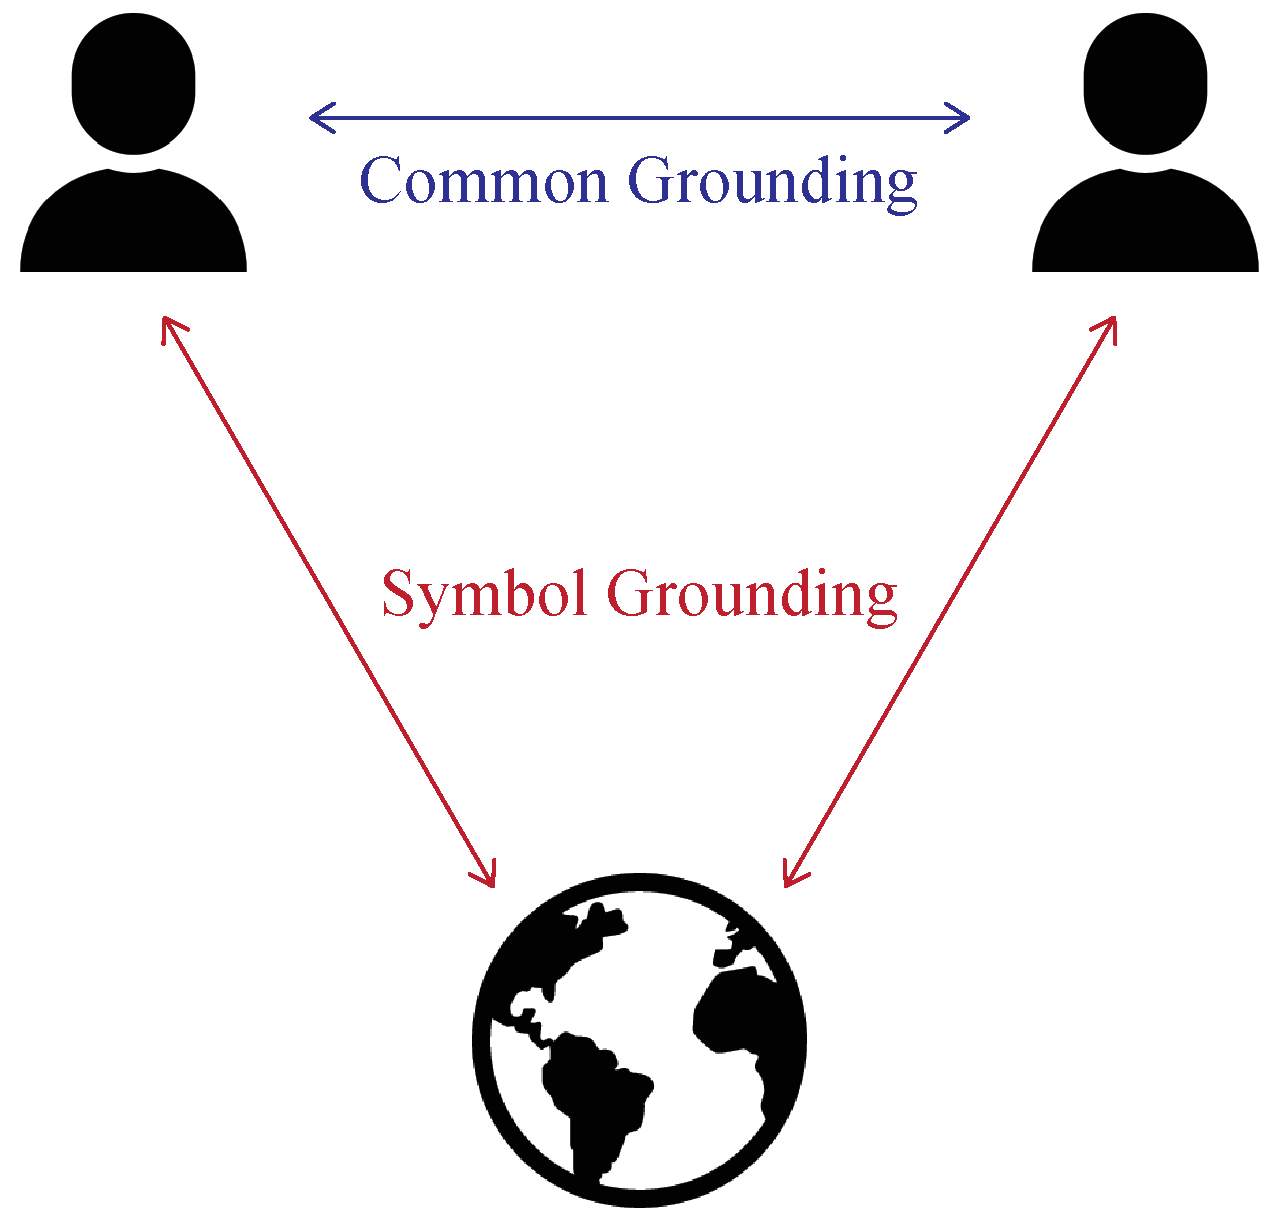
\includegraphics[width=0.5\textwidth]{triadic_relations.pdf}
\caption{The triadic relations of common grounding and symbol grounding.
}
\label{02_fig:triadic_relations}
\end{figure*}

\subsection{Language Acquistion}
\label{02_subsec:language_acquisition}

The meaning of language cannot be defined by the language itself, as it would lead to an endless circular definition: instead, it must be somehow connected to the physical world in the right way \citep{harnad1990symbol}. At the same time, we cannot use language in an arbitrary way if we were to communicate with each other: the usage of language must become a \textit{convention} through the process of common grounding \citep{lewis1969convention}. These two requirements form an intricate triadic relationship in terms of constructing and acquiring natural language, as depicted in Figure \ref{02_fig:triadic_relations}.

This relationship has been noticed and investigated in a variety of literature. In developmental psychology, the establishment of \textit{joint attention} (mutual recognition of an external entity) has been regarded as a crucial basis for first language acquisition \citep{clark2001grounding,tomasello2009constructing}: this is a representative example where common grounding meets symbol grounding. In the fields of linguistics and AI, there has been an intense debate over the schools of nativism, empiricism and culturism \citep{Chomsky1957-CHOSS-2,elman1996rethinking,steels1997synthetic}. For instance, the naming of color in human language may be affected by the innate structure of our perception, the physical world and environments we experience, or the requirements as a social tool for communication \citep{Steels2005coordinatingPG}. The converging view seems to suggest that all of these perspectives matter, complexly involving innate human structures, symbol grounding and common grounding \citep{larsson2018grounding}.

On the other hand, the NLP community has been predominantly focusing on the study of static corpora. Such corpus-driven approach originates in the seminal work of Penn Treebank \citep{marcus-etal-1993-building} and often validated on the account of the \textit{distributional hypothesis}, known for the famous quote from \citet{firth1957synopsis} -- ``you shall know a word by the company it keeps''. This approach has been successful to a remarkable extent: state-of-the-art models achieve near human-level performance on a range of natural language understanding benchmarks \citep{wang-etal-2018-glue,devlin-etal-2019-bert}, even in the challenging few-shot settings \citep{NEURIPS2020_1457c0d6}. However, upon deeper inspection, their linguistic abilities often turn out to be brittle and shallow, as we've seen in the case with BlenderBot (c.f. Section \ref{02_subsec:tasks_and_datasets}). Consequently, increasing works caution that language acquisition cannot be realized only from its forms (corpora) and requires interaction with the real world and other humans \citep{bisk-etal-2020-experience,bender-koller-2020-climbing,benotti-blackburn-2021-grounding}. 

Building upon these backgrounds/observations, we make an important contribution to study the triadic relationship of common grounding and symbol grounding in a minimal yet advanced setting. To be specific, we focus on the primary notion of \textit{joint attention} and incorporate realistic factors of human dialogues in the physical environments: namely \textit{continuity}, \textit{partial-observability} and \textit{dynamics}.


\subsection{Spatio-Temporal Grounding}
\label{02_subsec:spatio_temporal_grounding}

While symbol grounding encompasses all conceivable connections between language and the physical world, one principal connection is made on the dimensions of space and time. This type of connection, which we refer to as \textit{spatio-temporal grounding}, has been an important subject of study at the intersection of CV and NLP.
\\

\noindent
\textbf{Visual Grounding Tasks}\quad
Vision-language grounding has been a longstanding goal in the fields of CV and NLP. This is fundamental for developing systems that can not only \textit{speak} but also \textit{perceive} and \textit{act} in the physical world, just as we normally do. Such technology is also crucial for making information accessible to the visually-impaired, e.g. by automatically rendering visual contents to natural language descriptions.

One representative task of visual grounding is the \textit{visual question answering (VQA)} task. This requires the models to answer correctly to the questions (information requests) related to the visual context, including images \citep{antol2015vqa,hudson2019gqa} as well as videos \citep{lei-etal-2018-tvqa,lei-etal-2020-tvqa}. In the \textit{visual captioning (VC)} task, the goal is to provide the descriptions of salient objects, events, background, etc in a given scene through natural language \citep{xu2015show,hossain2019comprehensive}. Finally, in \textit{visual dialogues}, the task is extended to an interactive setting, typically involving both the \textit{reactive} aspects of VQA and \textit{proactive} aspects of VC \citep{das2017visual,de2017guesswhat,alamri2019audio}.

However, realistic visual contexts are often unbalanced and lack diversity in terms of spatio-temporal relations. For instance, in natural photographs, a dog would most likely be \textit{under} a tree rather than \textit{on top of} a tree. In natural videos, a book would typically \textit{fall off} the shelf but not \textit{float up} to the shelf. When such biases exist, the spatio-temporal attributes and relations may be identifiable based on superficial clues only, e.g. by simply recognizing the object categories (\textit{dog}, \textit{tree}, \textit{book}, \textit{shelf}, etc) \citep{goyal2017making,cirik-etal-2018-visual}.

\begin{figure*}[t!]
\centering
\begin{minipage}{.5\textwidth}
  \centering
  \includegraphics[width=.93\textwidth]{clevr_sample.pdf}
\end{minipage}%
\begin{minipage}{.5\textwidth}
  \centering
  \includegraphics[width=.92\textwidth]{nlvr_sample.pdf}
\end{minipage}
\caption{Example questions from the CLEVR dataset \citep{johnson2017clevr} (left) and the NLVR dataset \citep{suhr2017corpus} (right).
}
\label{02_fig:clevr_nlvr_sample}
\end{figure*}

One solution to circumvent this issue is to use synthetic visual contexts. As an illustration, we show example instances from CLEVR \citep{johnson2017clevr} and NLVR datasets \citep{suhr2017corpus} in Figure \ref{02_fig:clevr_nlvr_sample}. In these datasets, the entity attributes and relations are restricted to preliminary concepts but randomly sampled in a fully controlled manner. This way, their \textit{combinatorial} variety is maximized while reducing exploitable biases, requiring genuine understanding and compositional generalization \citep{Fodor1988ConnectionismAC,Lake2018GeneralizationWS}. Furthermore, the controllability of the context allows for various in-depth analyses of complex models, e.g. error analyses and \textit{causal} analyses through direct intervention \citep{pearl2009causality,pearl2018book}.

While these two approches have complementary strengths and weaknesses, we generally follow the second line of research (based on synthetic contexts) to maximize the diversity of spatio-temporal expressions and enable faithful evaluation and diagnosis of spatio-temporal grounding.
\\

\noindent
\textbf{Spatio-Temporal Language}\quad
Finally, spatio-temporal language has a long history of research as well. In computational linguistics, annotation frameworks have been proposed to capture the events, time and temporal relations expressed in natural language, e.g. in news articles \citep{pustejovsky2003timeml,ning-etal-2018-multi}. The annotation of spatial language has also been attempted to capture the information related to locations, directions, topological relations and motions \citep{pustejovsky2011iso,dan-etal-2020-spatial}. The recognition of such spatio-temporal information plays a fundamental role in natural language comprehension \citep{zwaan1998situation} as well as pratical applications such as information extraction and text mining \citep{banko2007,Aggarwal2012MiningTD}.

In the CV community, one of the most popular representations of spatio-temporal information is based on the \textit{scene graphs} \citep{johnson2015image,krishna2017visual}. In this approach, spatio-temporal attributes and relations are captured in the \textit{predicate-argument structure}, as shown in Figure \ref{02_fig:scene_graph}. This allows for a natural mapping from spatio-temporal language to \textit{regions} (e.g. object boundaries) in the visual scenes.

\begin{figure*}[t!]
\centering
\includegraphics[width=0.6\textwidth]{scene_graph.pdf}
\caption{An example of the scene graph representation from \citet{johnson2015image}.}
\label{02_fig:scene_graph}
\end{figure*}

However, existing works mostly focus on \textit{monologues} rather than dialogues, ignoring the important intersection between symbol grounding and common grounding. In dialogues, speakers often have incomplete/asymmetric information, requiring collaborative coordination on the semantics, references, \textit{frames} of references, etc: for instance, the referent of the speaker may not be visible/groundable for the listener. To address such issues, interlocutors often rely on \textit{modifications} to express precise information \citep{paradis_2008} and \textit{ellipses} to make conversation efficient. 

These factors can make the application of existing approaches (e.g. annotation frameworks and scene graphs) nontrivial, yet mostly ignored in the prior literature (e.g. \citealt{elliott-keller-2013-image}). In this thesis, we explicitly take into account such complexities and propose a simple yet challenging testbed of spatio-temporal language in interactive conversations.


\graphicspath{{03_task_formulation/figures/}} % Location of the graphics files

\chapter{Task Formulation under Continuous and Partially-Observable Context}
\label{03_chp:task_formulation}

Common grounding is the process of creating, repairing and updating mutual understandings, which is a critical aspect of sophisticated human communication. However, existing dialogue systems still have limited capability of creating common ground, and we also lack task formulations which introduce natural difficulty of common grounding while enabling easy evaluation and analysis of complex models. In this chapter, we propose a minimal dialogue task which requires advanced skills of common grounding under \textit{continuous} and \textit{partially-observable} context. Based on this task formulation, we developed OneCommon Corpus: a large-scale dataset of 6,760 dialogues which fulfills essential requirements of natural language corpora. Through our dataset analysis, we uncover the difficulty of common grounding and other relevant phenomena that need to be considered. Finally, we evaluate and analyze baseline neural models on a simple subtask that requires accurate recognition of the created common ground. Our results show that the baseline models perform decently but leave room for further improvement.

\section{Introduction}
\label{03_sec:introduction}

One major goal of NLP is to develop systems with human-level competence of dialogue. In the field of psychology, the ability to construct and maintain common ground has been pointed out to be essential for natural language communication \citep{clark1996using} as well as acquisition \citep{tomasello2009constructing}. Furthermore, in human-computer interaction (HCI), it is important that humans and computers have certain ways of creating \emph{mutual understandings} to collaborate reliably \citep{brennan1998grounding}. Although natural language is not the only option, it is one of the most effective, effortless and versatile solutions to this problem.

\subsubsection{Problems of Existing Research}

However, existing study of common grounding in dialogue system research is limited in three major ways. First, existing dialogue tasks are limited in terms of common grounding due to the restricted types of information that need to be dealt with. Specifically, they are focused on either \emph{categorical} or \emph{fully-observable} context, which makes common grounding a relatively trivial task:

\begin{itemize}
  \item Under \emph{categorical} context \citep{bordes2017learning,he2017learning,lewis-etal-2017-deal}, information can be expressed by symbolic natural language with minimal ambiguity. For example, there could be little ambiguity in describing categorical attributes like discrete colors (``red'', ``blue'' and ``yellow''). However, under \emph{continuous} context, natural language usage becomes more nuanced and pragmatic (such as ``darker gray'' and ``almost black'') for precise semantic coordination.
  \item Under \emph{fully-observable} context \citep{zarriess-etal-2016-pentoref,de2017guesswhat}, it is usually given that every information about the context is shared among the agents. This makes common grounding easier because information of the context is already present in (or at least easily added to) their common ground. In contrast, under \emph{partially-observable} context, agents typically need to create common ground from minimal shared information, and there could be various misunderstandings or partial understandings that need to be resolved.
\end{itemize}

Another problem is the difficulty of evaluation and analysis. As the models acquire more flexibility, automatic evaluation becomes problematic \citep{liu2016,novikova2017} and interpretation of model behavior becomes more challenging. Since advanced common grounding requires high flexibility, it is expected that we will need reliable evaluation metrics and analysis methods in the process of comparing and improving different methods.

Finally, there are limitations of model capabilities. Although traditional dialogue systems rely on rule-based engineering and predetermined slot-filling \citep{traum1994computational,young2013pomdp,williams2016dialog}, these models lack flexibility in terms of representing dialogue states and generating natural utterances. Since common ground can be very complex involving high ambiguity, uncertainty, partial understandings and misunderstandings, we need systems that can better capture such complexities and resolve them through flexible dialogues.

\subsubsection{Our Contributions}

In this chapter, we make a first step towards addressing these problems in the following ways. First, we formulate a novel dialogue task which requires advanced skills of common grounding under \emph{continuous} and \emph{partially-observable} context. Our task is based on a more general \emph{collaborative reference task}, where the goal of the agents is to coordinate attention on the same entity in a given context. This setting enables clear evaluation based on the task success rate and various error analyses of arbitrary models, since the contexts are simple and completely controllable (Section \ref{03_sec:task_formulation}).

Second of all, to enable the development of recent end-to-end dialogue systems with high flexibility \citep{bordes2017learning,lewis-etal-2017-deal}, we collected a large-scale dataset of 6,760 human-human dialogues with over 32K utterances through crowdsourcing on Amazon Mechanical Turk. During the dataset collection, we defined and managed to fulfill three essential requirements of natural language corpora: namely interpretability, linguistic/strategic variety and reliability (Section \ref{03_sec:dataset_collection}).

Next, we conduct comparative analyses with the previous dataset to illustrate how continuous and partially-observable context introduces difficulty in terms of common grounding. In addition, we conduct further analyses of the dataset to investigate the common grounding strategies at different levels, including nonlinguistic bias towards \emph{joint saliency} (Section \ref{03_sec:dataset_analysis}).

Finally, we evaluate and analyze simple neural network models on our dataset based on an important subtask of collaborative reference. Due to the complexity of common grounding, there remains huge room for further improvement (Section \ref{03_sec:experiments}).

Overall, the contributions of this chapter are as follows:

\begin{itemize}
  \item We proposed a simple and general idea of incorporating continuous and partially-observable context to the dialogue tasks, which makes common grounding difficult in a natural way.
  \item Following this idea, we formulated a minimal collaborative reference task which enables clear evaluation and analysis of complex models.
  \item We collected a large-scale dataset of 6,760 dialogues, which fulfills essential requirements of natural language corpora.
  \item Our analysis of the dataset verified the difficulty of common grounding and revealed various phenomena that need to be considered.
  \item We evaluated simple baseline models on an important subtask of collaborative reference and demonstrated huge room left for improvement.
\end{itemize}

\section{Task Formulation}
\label{03_sec:task_formulation}


\begin{figure}[th!]
\center
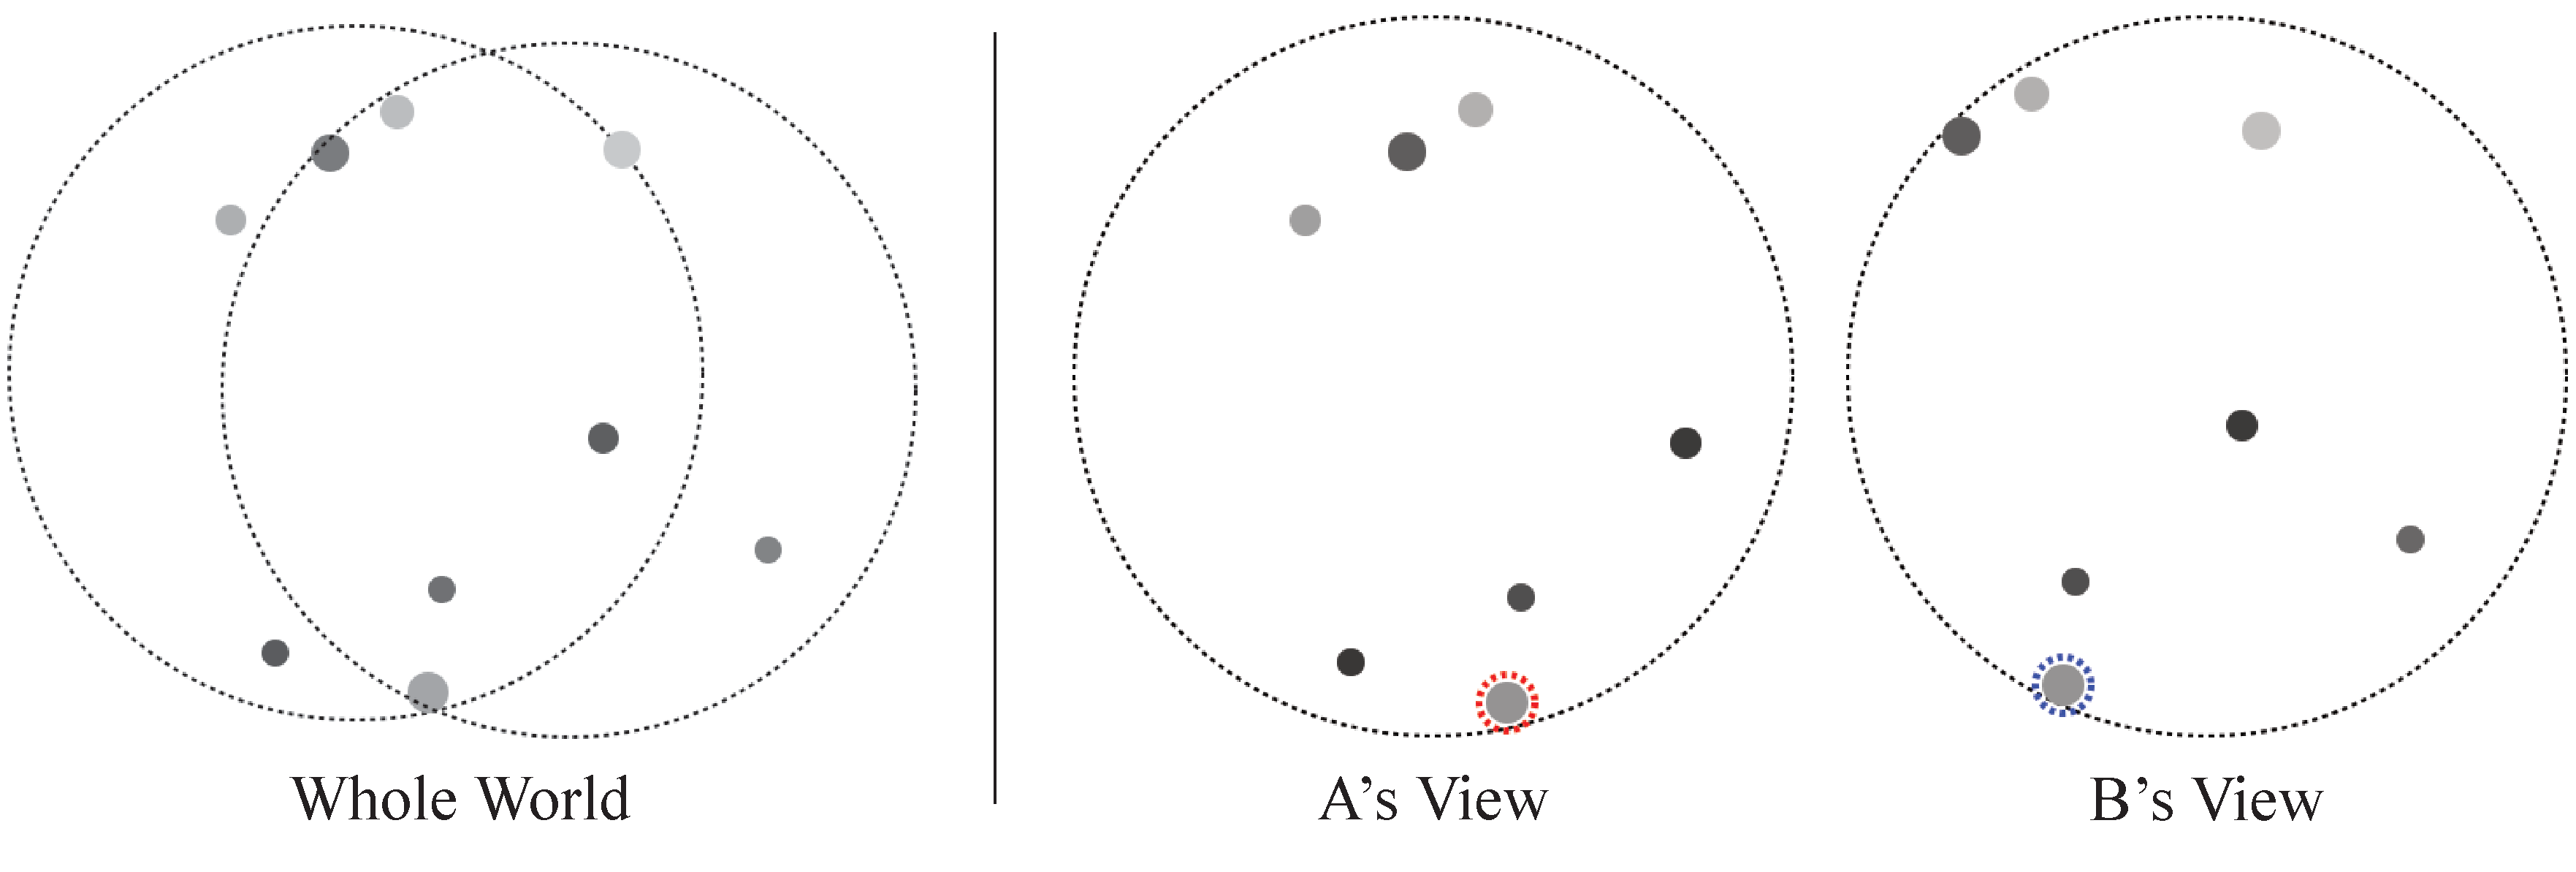
\includegraphics[width=\columnwidth]{onecommon_example.pdf}
\scalebox{0.95}{
\small
\begin{tabular}{@{}l@{}}
\toprule
A: I see three in a line going up and to the right. The middle one is the largest and darkest \\
B: I don't see that. I have one large, medium gray dot that's under a small, darker gray dot \\
A: Is the larger dot slightly to the left \\
B: yes, slightly, let's choose the larger one. \\
A: SELECT {\color{red} red} \\
B: SELECT {\color{blue} blue} \\
\bottomrule
\end{tabular}
}
\caption{An example dialogue of our collaborative reference task. Two agents have partial (overlapping) observations of a 2-D plane with 7 entities in each view. Their goal is to find and select the same entity through natural language communication.
}
\label{03_fig:onecommon_dialog}
\end{figure}

A \textit{collaborative reference task} is a multi-agent cooperative game with entities $E = \{e_1, e_2, ... , e_m\}$ and agents $A = \{a_1, a_2, ... , a_n\}$. Each agent $a_i \in A$ has an observation of $E$, and they can freely exchange information with other agents in natural language. At the end of the game, each agent selects one of the observable entities, and the game is considered \emph{successful} if and only if all the agents selected the same entity. This is a general framework for evaluating accurate \textit{mutual recognition} of a common entity, which is often a critical step in general common grounding.

Note that in contrast to the typical reference tasks \citep{kazemzadeh2014referit,de2017guesswhat}, agent roles are \textit{symmetric} and they can agree on any of the common entities (as long as it's the same). A dataset closest to our setup is the MutualFriends dataset \citep{he2017learning}, which is based on the task of finding a mutual friend from private lists of friends. Although this can be considered as a collaborative reference task under \emph{partially-observable} context (due to the privacy of knowledge), they only include \emph{categorical} information and the difficulty of common grounding is limited. 

Based on this task formulation, we propose a minimal task setting under \emph{continuous} and \emph{partially-observable} context. To be specific, we consider two agents and multiple entities located on a 2-D plane. Each entity has 3 simple attributes (2-D location, size and color) represented as \textit{continuous} real values. Furthermore, the agents are located slightly differently on the plane, and they can only observe the entities within a fixed radius: this way, our setting is made \textit{partially-observable} as well. 

We show an example dialogue of our task in Figure \ref{03_fig:onecommon_dialog}. Although human players successfully coordinated their selections with a short number of utterances, we can verify advanced common grounding strategies such as pragmatic expressions (\utterance{three in a line going up}), clarifications based on hypothesis testing (\utterance{Is the larger dot slightly to the left}) and nuanced acknowledgements (\utterance{yes, slightly}).

For the sake of simplicity, the number of entities observable by each agent is fixed at $7$. This ultimately reduces our task to a simple \textit{classification} problem, which can be evaluated based on simple metrics (such as accuracy).


\section{Dataset Collection}
\label{03_sec:dataset_collection}

We basically followed the dataset collection procedure of the MutualFriends dataset \citep{he2017learning}. We used Amazon Mechanical Turk to pair up 2 crowd workers and gave 20 seconds to read an example dialogue, followed by a maximum of 6 minutes session to complete the task. Our chat interface is shown in Figure \ref{03_fig:annotation}.

\begin{figure}[ht]
\centering
\vspace{1mm}
\includegraphics[width=0.95\columnwidth]{annotation.pdf}
%\vspace{1mm}
\caption{
A screenshot of our chat interface. Workers are given a maximum of 6 minutes to identify one of the common entities through dialogue.
}
\label{03_fig:annotation}
\end{figure}

In this procedure, we were concerned with three essential requirements of natural language corpora: namely \emph{interpretability}, \emph{linguistic/strategic variety} and \emph{reliability}. In the following, we discuss the importance of each requirement as well as how we managed to fulfill them:
\\

\noindent
\textbf{Interpretability}\quad
We define the interpretability of the dataset to be the ease of interpreting its language and strategy, which is critical for conducting annotations and further analyses. However, \emph{lack of discipline} and \emph{complexity of the vocabulary} can make corpora difficult for interpretation.

In free-formed dialogues, lack of discipline can cause unnecessary difficulty in terms of interpretation. For instance, \emph{cross-talk} (conversation which does not progress sequentially) can occur frequently \citep{he2017learning} and complicate important structures of dialogues, such as discourse segments, adjacency pairs and \emph{contributions} in common grounding \citep{clark1989contributing}. Hence, we minimized them by forcing workers to take turns. Also, \emph{chit-chat} could occur occasionally, which adds undesirable noise for analyzing common grounding. Therefore, we explicitly instructed the workers to avoid talking about things that are irrelevant to this task.

Keeping the vocabulary simple is also important for interpretability, especially for people unfamiliar with the domain. For instance, the MutualFriends dataset includes up to 7 attributes with approximately 3K complex named entities and technical terms. In contrast, we kept the entity attributes minimal with only 3 simple and intuitive properties (location, size and color). As a result, this greatly reduced the complexity of the vocabulary as we describe in Section \ref{03_sec:dataset_analysis}.
\\

\noindent
\textbf{Linguistic and Strategic Variety}\quad
\emph{Linguistic and strategic variety} of the dataset is fundamental for developing dialogue systems with broad coverage. To satisfy this requirement, we sampled all entity attributes randomly from fixed uniform distributions, with the only restriction that the entities cannot be too close to each other. As the previous work with the similar idea confirmed \citep{suhr2017corpus}, we found rich varieties of linguistic phenomena, including cardinalities (\utterance{\textit{three} gray dots}), existentials (\utterance{\textit{There is} another small dark ..}), universals (\utterance{\textit{all} of the other dots are larger}), coordinations and negations (\utterance{further to the right \textit{and} \textit{not} as far down}).

During the dataset collection, we assigned 6,759 unique contexts to 6,760 dialogues we collected. We collected 2 dialogues based on the exact same context and confirmed that they solved the task in different ways. This suggests that there could be various effective solutions and the agents must adapt flexibly to their partners' strategies.

Finally, we incorporated variation in terms of the \textit{degree} of partial observability. Specifically, each agent has 7 entities in the view, but only 4, 5 or 6 of them would be in common. This introduces a further variation of common grounding strategies, as we discuss in detail in Section \ref{03_sec:dataset_analysis}.
\\

\noindent
\textbf{Reliability}\quad
Finally, we regard the \emph{reliability} of the dataset to be crucial, especially when crowdsourcing data with potentially careless, low-motivated workers. In fact, in our preliminary experiment, we found many cases where workers did not follow the instruction carefully or solve the task effectively (especially on difficult cases).

As a solution, we manually reviewed all works and rejected ones which clearly did not follow the instruction. Our instruction is kept brief and explicit so that it is easier to follow, and we also gave manual feedback about general solutions to improve their work. To discourage premature guessing, we prohibited workers from selecting within the first minute and instructed them to make it \emph{very sure} they found the same entity before selection. We also incentivized task success with \$0.05 bonus for all successful dialogues, in addition to the base reward of \$0.30.

As a result, we found significant improvement in terms of task success rate, which is an important evidence of the reliability of our dataset. \\

Based on the above procedure, we collected 6,839 dialogues, and after the reviewing process, we accepted 6,760 dialogues in total. We refer to this dataset as \textbf{OneCommon Corpus}. Overall, we received positive feedback from the crowd workers and they seemed to enjoy playing it, which is important from the aspect of gamification.

\section{Dataset Analysis}
\label{03_sec:dataset_analysis}

In this section, we first study the difficulty of common grounding in comparison to the previous settings. Secondly, we conduct further analyses to investigate other relevant phenomena that need to be considered.

\subsection{Difficulty of Common Grounding}
\label{03_subsec:difficulty_analysis}

Our hypothesis is that \emph{continuous} and \emph{partially-observable} context makes common grounding difficult compared to \emph{categorical} or \emph{fully-observable} context. However, it is relatively obvious that \emph{fully-observable} setting would make collaborative reference trivial: for instance, if our task was fully-observable, one can easily succeed by always uttering \utterance{\textit{select the leftmost dot}}. Therefore, we mainly focus on assessing how \textit{continuous} context adds difficulty in terms of common grounding.

As a comparison, we use the MutualFriends dataset which is based on a similar collaborative reference task under partially-observable but \emph{categorical} context \citep{he2017learning}. However, several differences make a direct comparison difficult: for instance, we only gave one chance for the entity selection, while the MutualFriends dataset allowed multiple chances in the given amount of time. Therefore, we focus on the following factors which are less affected by such differences.

\subsubsection{Utterance Lengths}

\begin{table*}[ht]
\centering \scalebox{0.81}{
%\setlength\tabcolsep{9pt}
\setlength{\aboverulesep}{0pt}
\setlength{\belowrulesep}{0pt}
\setlength{\extrarowheight}{.2ex}
\begin{tabular}{c|cccc}
\toprule
 & \multirow{2}{*}{MutualFriends} & \multicolumn{3}{c}{OneCommon} \\
 & & \#Shared=4 & \#Shared=5 & \#Shared=6 \\
\midrule
Total dialogues &
10,661 & 2,189 & 2,279 & 2,292 \\
Average tokens per utterance&
5.38 & 12.87 & 12.37 & 11.86\\
Average utterances per dialogue&
8.97$^*$ & 4.97 & 4.77 & 4.56 \\
Success rate (\%) &
0.85$^*$ & 0.66 & 0.77 & 0.87 \\
\midrule
Unique tokens & 13,478 & \multicolumn{3}{c}{3,761} \\
Occupancy of top 10\% frequent tokens (\%) & 91.6\% & \multicolumn{3}{c}{97.0\%} \\
\bottomrule
\end{tabular}
}
\caption{\label{03_tab:statistics}
Basic statistics of our dataset and the MutualFriends dataset \citep{he2017learning}. To count tokens and vocabulary size, we preprocessed the text with the same NLTK word tokenizer \citep{nltkbook} and converted each token to its lowercased form. ($^*$ denotes where direct comparison is not suitable due to the task difference.)
}
\end{table*}

First, we compare the \emph{average utterance length} because this indicates the syntactic/semantic complexity of utterances required for common grounding. As shown in Table \ref{03_tab:statistics}, utterances in our dataset are at least twice as long compared to the MutualFriends dataset: this indicates that more complex utterances are required under continuous context to make the descriptions precise. We also found that the utterance lengths slightly increase when the number of shared entities is smaller: this suggests that (a greater degree of) partial-observability also adds complexity at the utterance level.

\subsubsection{Pragmatic Expressions}

\begin{figure}[th!]
\centering
\begin{tikzpicture}
\node[inner sep=0pt] (agent_0) at (0,0)
  {\includegraphics[width=0.35\columnwidth]{S_VdQsGMpy6Su1tzIy_agent_0.pdf}};
\node[inner sep=0pt] (agent_1) at (6,0)
  {\includegraphics[width=0.35\columnwidth]{S_xJimjRbmhtdjZbNl_agent_1.pdf}};
\node [below] at (0,-2.5) {large \textbf{black} dot};
\node [below] at (6,-2.5) {a close \textbf{triangle}};
\end{tikzpicture}
\caption{
Examples of typical pragmatic expressions in our dataset (marked by bold).
}
\label{03_fig:pragmatics}
\end{figure}

In our dataset, we found many \emph{pragmatic expressions} whose meaning depends on the context and should not be taken literally. A typical example is the usage of the word ``black'' to indicate the darkest dot in the context, even if its color is not completely black. Another common expression ``triangle'' is also pragmatic, since in the literal sense there could be numerous triangles in one's view, and the speaker actually indicates a group of three dots which is the closest to a \textit{prototypical} type of triangles, such as an equilateral triangle. We show some illustrating examples in Figure \ref{03_fig:pragmatics}.

As the previous work pointed out, such pragmatic expressions are characteristic under continuous context \citep{monroe2017colors} and add complex ambiguity/uncertainty that need to be resolved through common grounding.

\subsubsection{Nuanced Expressions}

Finally, the frequent usage of \emph{nuanced} expressions is an important characteristic of our dataset. Since the context is continuous and partially-observable, we hypothesize that speakers need to rely on such expressions to express subtle differences in terms of degree, ambiguity, uncertainty, and so forth.

To estimate the frequency of nuanced expressions, we follow \citet{paradis_2008} and define 2 main types (and 5 subtypes) of degree modifiers: \textit{scalar modifiers} used for concepts in a range of scale (\textit{diminishers}, \textit{moderators}, \textit{boosters}) and \textit{totality modifiers} used for concepts with definite boundaries (\textit{approximators}, \textit{maximizers}). See Figure \ref{03_fig:degree_modifiers} for the proposed taxonomy and examples of such degree modifiers.

\begin{figure}[th!]
\center
\vspace{2mm}
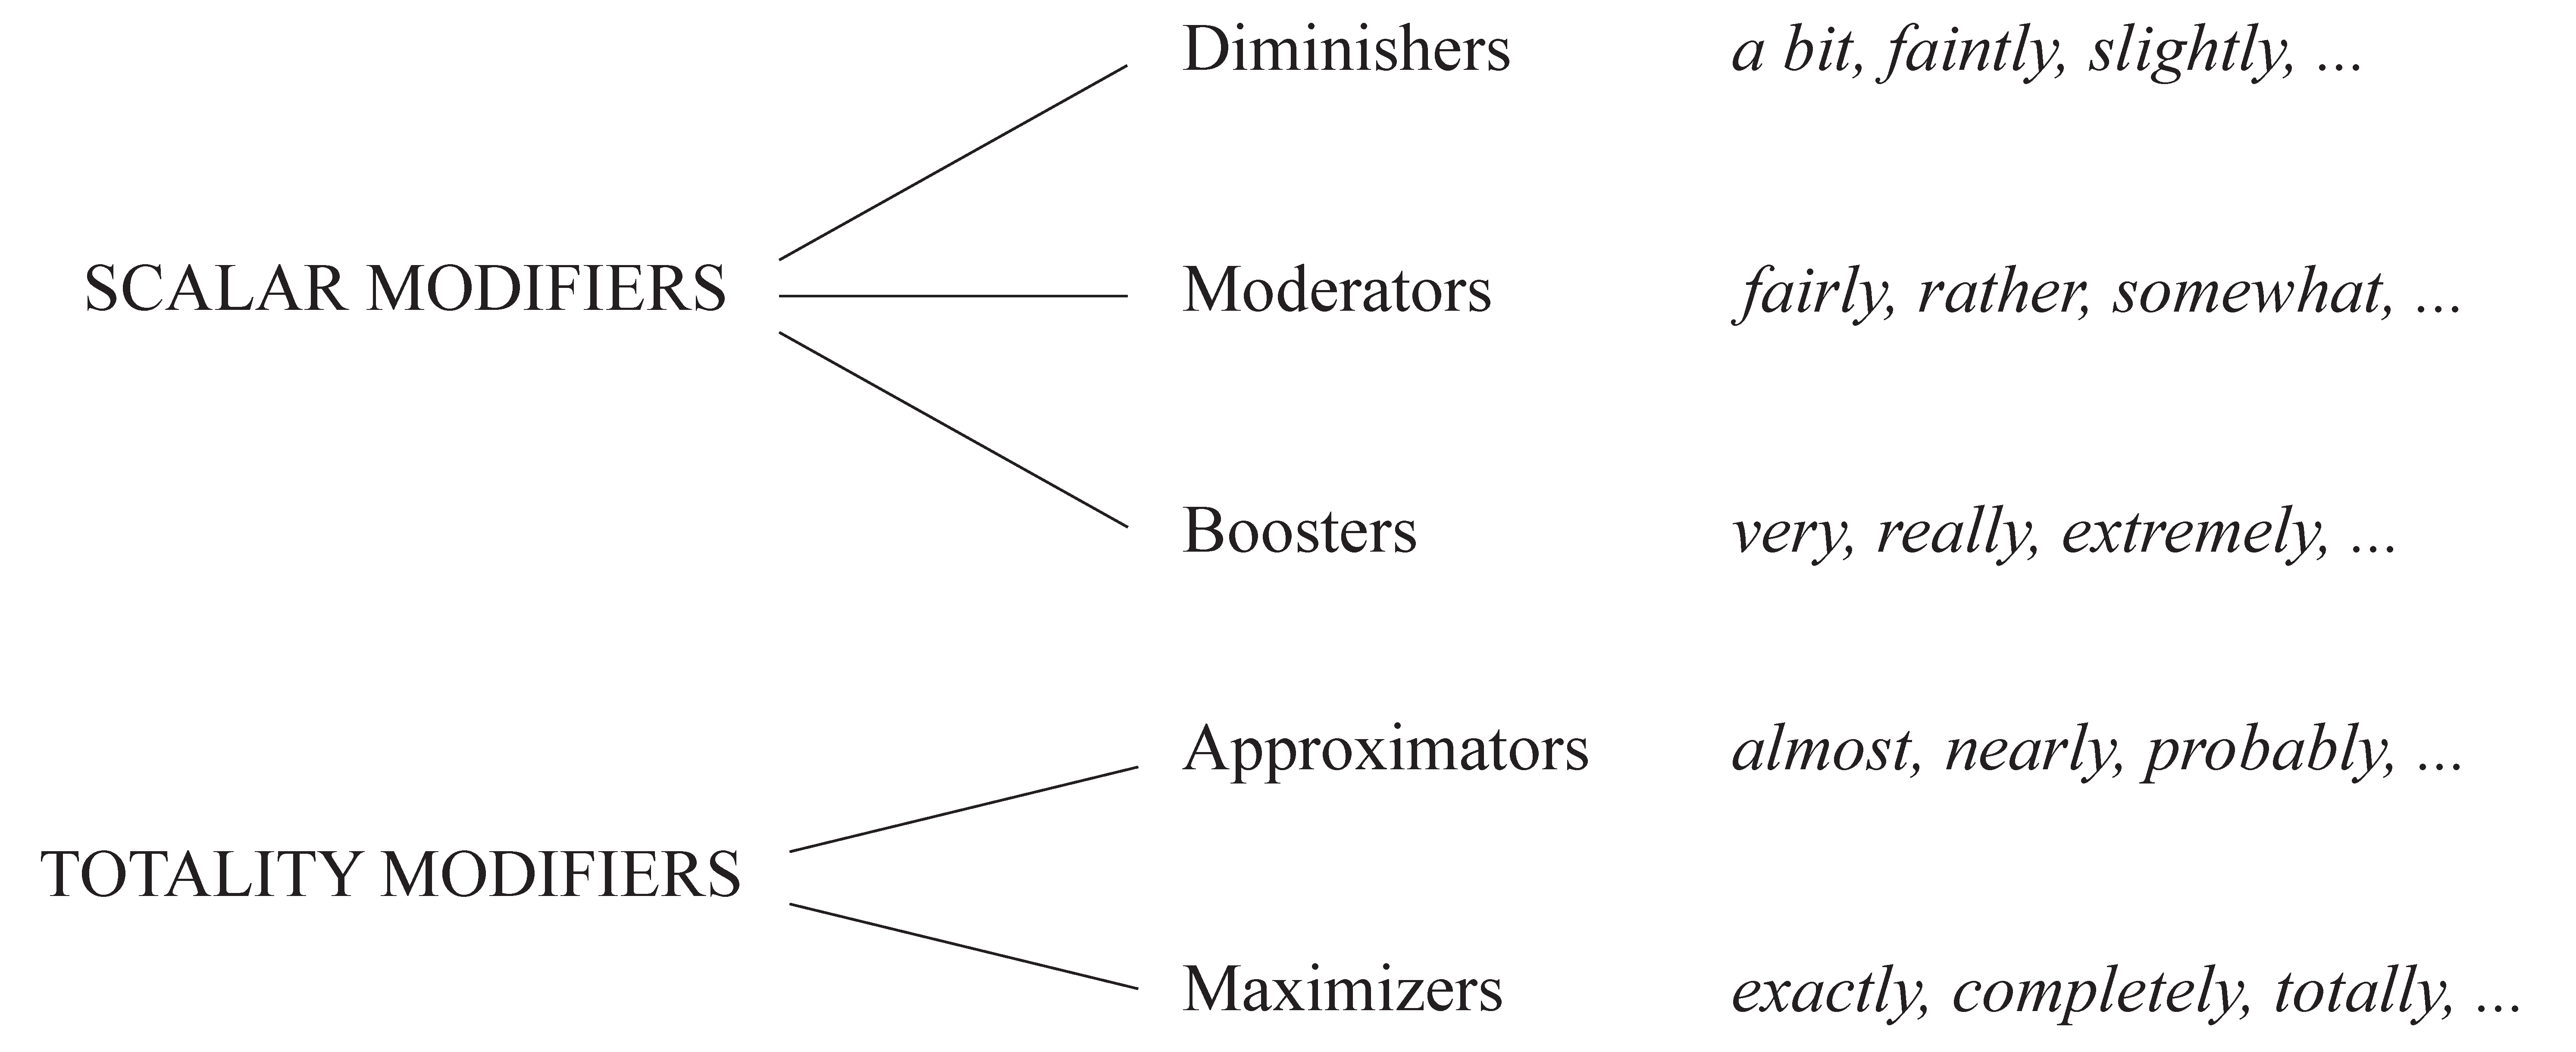
\includegraphics[width=0.97\columnwidth]{degree_modifiers.pdf}
\vspace{1mm}
\caption{A taxonomoy of the degree modifiers based on \citet{paradis_2008}.
}
\label{03_fig:degree_modifiers}
\end{figure}

Based on this taxonomy, we manually created a keyword-based dictionary of the degree modifiers. Note that we excluded words which are likely to be used with different meanings (such as ``like'', ``about'' and ``around'') and do not consider nuances expressed morphologically (such as \textit{-ish} as in ``small\textit{ish}''), although they are also common in our dataset. Using this dictionary, we estimated the frequency of the modifiers in the MutualFriends dataset and OneCommon Corpus. As shown in Table \ref{03_tab:nuances}, we can verify that our dataset includes significantly more degree modifiers of various types, which are used effectively to cope with ambiguity and uncertaintiy. \\

\begin{table*}[t!]
\centering \scalebox{0.83}{
\setlength\tabcolsep{9pt}
\setlength{\aboverulesep}{0pt}
\setlength{\belowrulesep}{0pt}
\setlength{\extrarowheight}{.4ex}
\begin{tabular}{c|cc|cl}
\toprule
Degree Modifiers & MutualFriends & OneCommon & \# Keywords &  \multicolumn{1}{c}{Usage in OneCommon} \\
\midrule
Diminishers & 0.01 & 9.19 & 10 & \textbf{slightly} to the right \\
Moderators & 0.09 & 1.28 & 6 & \textbf{fairly} close together \\
Boosters & 0.17 & 9.83 & 27 & \textbf{very} light dot \\
Approximators & 0.86 & 10.23 & 34 & \textbf{almost} in the middle \\
Maximizers & 0.47 & 4.31 & 37 & \textbf{exactly} horizontal \\
\bottomrule
\end{tabular}
}
\caption{\label{03_tab:nuances}
Average occurrences of degree modifiers per 100 utterances (estimated based on keywords).
}
\end{table*}

To summarize our analyses, utterances are much longer in our dataset, which indicates the complexity of common grounding at the utterance level. In addition, our dataset involves more ambiguity and uncertainty represented by the frequent usage of pragmatic and nuanced expressions. These observations verify that common grounding becomes more difficult and complicated under continuous and partially-observable context.

On the other hand, we found that human workers could solve the task reasonably well with little evidence of confusion. Therefore, we conclude that our task setting is fundamental for adding natural difficulty in terms of common grounding.

\subsection{Other Relevant Phenomena}

Next, we conduct further analyses of the dataset and investigate various phenomena related to common grounding that need to be considered.

\subsubsection{Basic Statistics}

From Table \ref{03_tab:statistics}, we also found that dialogues get longer in terms of the \emph{(average) number of utterances} when a fewer number of entities is shared. This shows that under a greater degree of partial-observability, it is more likely that the presented information is not \emph{groundable}, and players need more interaction (try-and-error) to create common ground. We can also see that the success rate drops naturally, so in general common grounding becomes more challenging when less information is shared.

In terms of lexical variety, our dataset contains 3,761 unique tokens in total, in contrast to 13,478 in the MutualFriends dataset. In addition, we found that a large portion of our dataset consists of common words: to be specific, the top 10\% of the most frequent tokens occupy 97.0\% of the whole tokenized corpus, in contrast to 91.6\% in the MutualFriends dataset. These suggest that the vocabulary of our dataset is extremely simple, which is an important evidence of interpretability discussed in Section \ref{03_sec:dataset_collection}. This may also be helpful for training dialogue systems, since rare words are less problematic.

\subsubsection{Nonlinguistic Phenomena}

Language is a \emph{coordination device} we use to coordinate our joint actions \citep{lewis1969convention}, but we also use \emph{joint saliency} to coordinate actions at the nonlinguistic level \citep{Schelling1960}. In our dataset, we found that human players have a tendency to focus attention on \emph{perceptually} salient entities more often.

To demonstrate this, we plot the final selection probabilities of the entity's color and size in Figure \ref{03_fig:plot-select}. We can clearly see that the selections are biased, and entities with extreme properties (around the edge) are more likely to be selected. We also found that darker entities are more likely to be selected (62.7\%) compared to lighter entities (37.3\%), and larger entities (54.3\%) slightly more likely than smaller entities (45.7\%).

There could be other types of joint saliency as well (such as geometric relations between entities), but the point is that such bias exists and needs consideration: for example, just by taking advantage of such bias, we can predict human selections significantly better than random (Section \ref{03_sec:experiments}). However, due to the \textit{partially-observability}, joint saliency is not sufficient and communication is critical to solving our task.

\begin{figure}[t!]
\centering
\includegraphics[width=0.74\columnwidth]{selection_bias.pdf}
\caption{
Final selection probabilities based on color and size. The total range of size is 7 and color is split into 30 equal-sized bins in grayscale (smaller is darker).
}
\label{03_fig:plot-select}
\end{figure}

\subsubsection{Utterance Level Phenomena}

Understanding speaker's intention at the \emph{utterance level} is critical in dialogue \citep{grice1957meaning}: especially the idea of speech act \citep{austin1962things,searle1969speech} has been applied widely in dialogue system research to improve natural language understanding and generation \citep{yao2013recurrent,hakkani2016multi}.

During data collection, we allowed free-formed conversation with minimal restrictions, as long as they are relevant to the accomplishment of the task. As a result, we found a wide variety of speech acts in the course of common grounding. We show illustrative examples of the collected utterances in Table \ref{03_tab:speechact}. Utterances are grouped by the \textit{communicative functions} defined in \citet{bunt2017dialogue}, including \textit{information transfer functions} (\textit{information provision/request}) and \textit{action discussion functions} (\textit{commissives/directives}). With additional annotations, our dataset can be easily extended to study such pragmatic structures as well \citep{stolcke-etal-2000-dialogue}.

\begin{table*}[th!]
\centering \scalebox{0.82}{
\begin{tabular}{lcl}
\toprule
Function & Type & Example Utterances\\
\midrule
\multirow{8}{*}{Info. Provision} & \multirow{1}{*}{Inform (Init.)} & I have very dark small dot in the center \\
& \multirow{1}{*}{Inform (Cont.)} & It also has a small light grey one further down from the group \\
& \multirow{1}{*}{Agreement} & Yes I have one like that. / same here. \\
& \multirow{1}{*}{Agreement (Strong)} & Exactly! / perfect. mine too. \\
& \multirow{2}{*}{Agreement (Partial)} & not sure its the one / more of a line. \\
& & Yes, but the small is medium dark, not completely black \\
& \multirow{1}{*}{Disagreement} & I don't have that one. / mine are not in those locations. \\
\midrule
\multirow{4}{*}{Info. Request} & \multirow{1}{*}{Question (Prop.)} & the middle one is the darkest of the 3? \\
& \multirow{1}{*}{Question (Set)} & where is it in relation to the large med grey? \\
& \multirow{1}{*}{Question (Choice)} & Which should we choose? / the black or the grey? \\
& \multirow{1}{*}{Question (Check)} & It's the darkest dot in the circle, right? \\
\midrule
\multirow{1}{*}{Commissives} & \multirow{1}{*}{Offer} & lets click the upper left one that's bigger and darker gray \\
\midrule
\multirow{2}{*}{Directives} & \multirow{1}{*}{Request} & tell me about your tiniest dot? / pick one at the bottom \\
& \multirow{1}{*}{Suggestion} & Please describe it in relation to other dots in the circle \\
\bottomrule
\end{tabular}
}
\caption{\label{03_tab:speechact}
Illustrative utterances in the dataset, grouped by the \emph{task dimension} of communicative functions \citep{bunt2017dialogue}}
\end{table*}

\subsubsection{Discourse Level Phenomena}

Finally, we found many coreferences and anaphoric expressions in our dataset. \emph{Coreference resolution} is the task of finding the mentions (referring expressions) in the dialogue with the same referents \citep{ng-2010-supervised}. In our dataset, we found two characteristics that complicate this task. First, due to the continuous and partially-observable context, mentions are usually ambiguous and the referents could be missing from one's view. Hence, players must keep track of various possibilities and disambiguate them through interaction. Secondly, players often use the \emph{grouping} strategy (such as ``three in a line'', ``a cluster of 4 dots'') where the mention can refer to a \emph{set} of multiple entities. This is a natural and effective strategy but adds complexity in terms of coreference resolution.

On the other hand, \emph{anaphora resolution} is the task of idenfitying the relation between a mention (\textit{antecedent}) and a succeeding mention (\textit{postcedent}) that depends on the previous mention \citep{poesio2016anaphora}. This can occur both within utterances (\utterance{a medium size black one, with a very light slightly smaller one to \textit{its} left}) and across utterances (\utterance{Does \textit{the lighter dot} appear to be slightly larger?}). In \textit{associative anaphora}, the referents of the postcedent can be different from the antecedent, e.g. only refer to a \textit{part of} the antecedent (as in \utterance{I have a pair where \textit{the left one} is large and dark}).

These discourse-level phenomena play a fundamental role in the process of common grounding and will be the main focus of our study in Chapter \ref{04_chp:interpretation}.

\section{Experiments}
\label{03_sec:experiments}

\subsection{Evaluation}

In this experiment, we focus on a simple subtask of common grounding, which we refer to as the \textbf{target selection task}. Specifically, our goal is to predict which target entity a human player selected, provided the player's private observation and the corresponding dialogue. This is an essential subtask of collaborative reference, where the player makes the final selection based on the established common ground. 

Since the number of entities in each player's view is fixed at 7, we can formulate this as a simple classification problem. However, we expect that even the accurate recognition of the target (i.e. common ground) would be challenging due to the complexity of common grounding strategies (as we discussed in Section \ref{03_sec:dataset_analysis}).

\subsection{Model Architecture}

As a preliminary experiment, our baseline models are kept as simple as possible with minimal preprocessing and hyperparameter tuning. The two main components of the models are as follows:

\subsubsection{Context Encoding}
The dialogue context (agent's view) is represented as a 28-dimensional real-valued vector, where each of the 7 observable entities is represented as a 4-dimensional vector (x-value, y-value, size, color). As a preprocessing step, we normalize each dimension of the vector in the range of $(-1, 1)$.


The simplest way to encode this is to directly apply a multi-layered perceptron (MLP) over the context vector. However, without feature engineering, this simple approach may have difficultly capturing relevant information, such as the \textit{relations} between entities. Therefore, in the second approach, we use the Relation Network \citep{santoro2017simple} to create additional features for the relations between entities. Specifically, we encode each \textit{pair} of the entities with a shared MLP (for a total of 21 pairs) and append the sum of these vectors as an additional input.

\subsubsection{Dialogue Encoding}

Utterances are all tokenized and lowercased, and tokens which occur less than 10 times are treated as a unique \emph{unknown} token. We insert a token which represents the \emph{speaker id} to each utterance at the beginning, and another token to indicate the end of the dialogue. Then, we embed each token with a shared MLP and run a bidirectional GRU \citep{cho2014properties} over the embedded tokens. Finally, we take the last state of the bi-GRU as the final representation (encoding) of the dialogue. \\

For prediction, we simply concatenate the context and dialogue encodings and run another MLP. However, as we've seen in Section \ref{03_sec:dataset_analysis}, there exists nonlinguistic selection bias in our dataset which makes predictions possible without using linguistic information (i.e. dialogue encoding). Therefore, as an ablation study, we also train the models to make predictions based on the context encodings only.

Following common practice, we split the dataset into training, validation and test set with a proportion of 8:1:1, and all models are tuned on the validation set. The loss function is calculated using cross entropy. All components of the neural networks are single-layered with 128 hidden units, and a dropout rate of 0.5 is applied at each layer to avoid overfitting. All parameters are initialized uniformly within the range of $(-0.01, 0.01)$. Models are trained with the Adam optimizer \citep{Kingma2015AdamAM} with an initial learning rate of 0.001, and we clip gradients whose $L^2$ norm is greater than 0.1. The experiment is run 10 times initialized with different seeds, and we report the mean and standard deviation of the selection accuracies on the full test set.

For further analyses, models with the best validation loss in the previous experiment are also evaluated on two variants of the test set. First, since the current test set contains correlated predictions on the same dialogue from the two players, we create the \textit{uncorrelated} test set by randomly removing one of the player's prediction. Secondly, we further removed dialogues where players failed to coordinate on the same entity to create the \textit{success-only} test set. The statistical significance of the results are computed on the uncorrelated test set using paired student's t-test.

Finally, we take 100 random samples from the uncorrelated test set (including 76 successful dialogues) to report human performance based on the average accuracy of two annotators.

\subsection{Results}
\label{03_subsec:results}

\begin{table*}[t!]
\centering \scalebox{0.83}{
\setlength\tabcolsep{9pt}
\setlength{\aboverulesep}{0pt}
\setlength{\belowrulesep}{0pt}
\setlength{\extrarowheight}{.4ex}
\begin{tabular}{c|ccc}
\toprule
 & Full & Uncorrelated & Success Only \\
\midrule
\midrule
Random & 14.28 & 14.28 & 14.28 \\
\midrule
Context Only (MLP) & 27.90 $\pm$ 0.6 & 28.74 & 29.59 \\
Context Only (MLP+RN) & 31.94 $\pm$ 0.9 & 30.22 & 32.40 \\
Context + Dialogue (MLP) & 40.27 $\pm$ 1.3 & 40.89 & 43.82 \\
Context + Dialogue (MLP+RN) & 43.09 $\pm$ 0.8 & 44.00 & 49.44 \\
\midrule
Human & - & 82.50 & 90.79 \\
\bottomrule
\end{tabular}
}
\caption{\label{03_tab:selection_experiment}
Results of the target selection task.
}
\end{table*}

We show the results of our experiment in Table \ref{03_tab:selection_experiment}. As we can see, models trained with the context encodings only perform significantly better than random (\textit{p}-value $<10^{-7}$). This verifies that we must indeed take into account the effect of selection bias when interpreting model performances.

Secondly, we found that encoding context with Relation Network (RN) consistently outperforms MLP, but not at a statistically significant level (\textit{p}-value $>0.1$). Therefore, the simplest strategy of using MLP works decently, but an improved architecture may potentially improve the overall performance.

Thirdly, models trained with both context and dialogue encodings significantly outperform models trained only with the context encodings (\textit{p}-value $<10^{-9}$). This indicates that even our simplest models can learn to leverage linguistic information along with the context to make better predictions.

Finally, we found that when the test set only includes successful cases, both the models and humans perform consistently better: however, human performance improves even more dramatically, achieving over 90\% accuracy. This indicates that the \textit{success-only} test set contains higher-quality dialogues with less noise.

Overall, our target selection task is challenging due to the complexity of common grounding, and we still have a huge room left for improvement.


\section{Conclusion}
\label{03_sec:conclusion}

In this study, we proposed a novel task setting under continuous and partially-observable context to require advanced strategies of common grounding. Based on this task setting, we formulated a minimal collaborative reference task to measure the ability of creating accurate common ground. To enable various empirical studies, we collected a large-scale dataset of actual human dialogues (OneCommon Corpus) through a careful crowdsourcing procedure. Our dataset analyses revealed the difficulties and distinct strategies of common grounding involved in our task. Finally, we developed and analyzed simplest baseline models based on the subtask of recognizing common ground. Due to the complexity of common grounding, we showed that there remains major room left for improvement in future work.


\graphicspath{{04_interpretation/figures/}} % Location of the graphics files

\chapter{Interpretation Based on Reference Resolution}
\label{04_chp:interpretation}

Interpreting the process of common grounding is a challenging task, especially under continuous and partially-observable context where complex ambiguity, uncertainty, partial understandings and misunderstandings are introduced. Interpretation becomes even more challenging when we deal with existing dialogue systems which still have limited capability of natural language understanding and generation. To address this problem, we consider reference resolution as the central subtask of common grounding and propose a new resource to study its intermediate process. Based on a simple and general annotation schema, we collected a total of 40,172 referring expressions in 5,191 dialogues curated from OneCommon Corpus, along with multiple judgements of referent interpretations. We show that our annotation is highly reliable, captures the complexity of common grounding through a natural degree of reasonable disagreements, and allows for more detailed and quantitative analyses of common grounding strategies. Finally, we demonstrate the advantages of our annotation for interpreting, analyzing and improving common grounding in baseline end-to-end dialogue systems.

\section{Introduction}
\label{04_sec:introduction}

Common grounding is the process of creating, repairing and updating mutual understandings, which is a critical aspect of sophisticated human communication \citep{clark1996using} as well as a longstanding goal in dialogue modeling \citep{traum1994computational}. Recently, there have been new proposals of dialogue tasks which require advanced skills of common grounding under \textit{continuous} and \textit{partially-observable} context \citep{udagawa2019natural,haber-etal-2019-photobook}. Their main contributions include the establishment of clear evaluation metrics (based on task success rates), collection of large-scale datasets and introduction of complex ambiguity, uncertainty, partial understandings and misunderstandings which are minimally observed under traditional (either categorical or fully-observable) context.

However, interpretation of the process of common grounding remains an open problem. Although formal approaches such as \citet{lascarides2009agreement} and \citet{poesio2010completions} account for some of the important details in common grounding, constructing such precise semantic representations is a difficult and costly process, especially under continuous and partially-observable context with high ambiguity and uncertainty. Interpretation becomes even more challenging when we deal with existing dialogue systems represented by the end-to-end dialogue systems \citep{vinyals2015neural,bordes2017learning}, which can converse fluently but still lack the true competence of natural language understanding and generation.

In this study, we approach this problem by \textit{decomposing} the common grounding task based on its intermediate subtasks. Specifically, we consider \textit{reference resolution} as the central subtask of common grounding (in the sense that mutual understanding can only be created through successful references), define this subtask formally based on a simple and general annotation schema, and create a large-scale resource to study this subtask along with the original task of common grounding.

Our annotated corpus consists of a total of 40,172 referring expressions in 5,191 dialogues curated from OneCommon Corpus \citep{udagawa2019natural}, along with multiple (a minimum of 3) judgements for referent interpretations. A visualization of our annotation is shown in Figure \ref{04_fig:first_example}.

\begin{figure*}[th!]
\centering
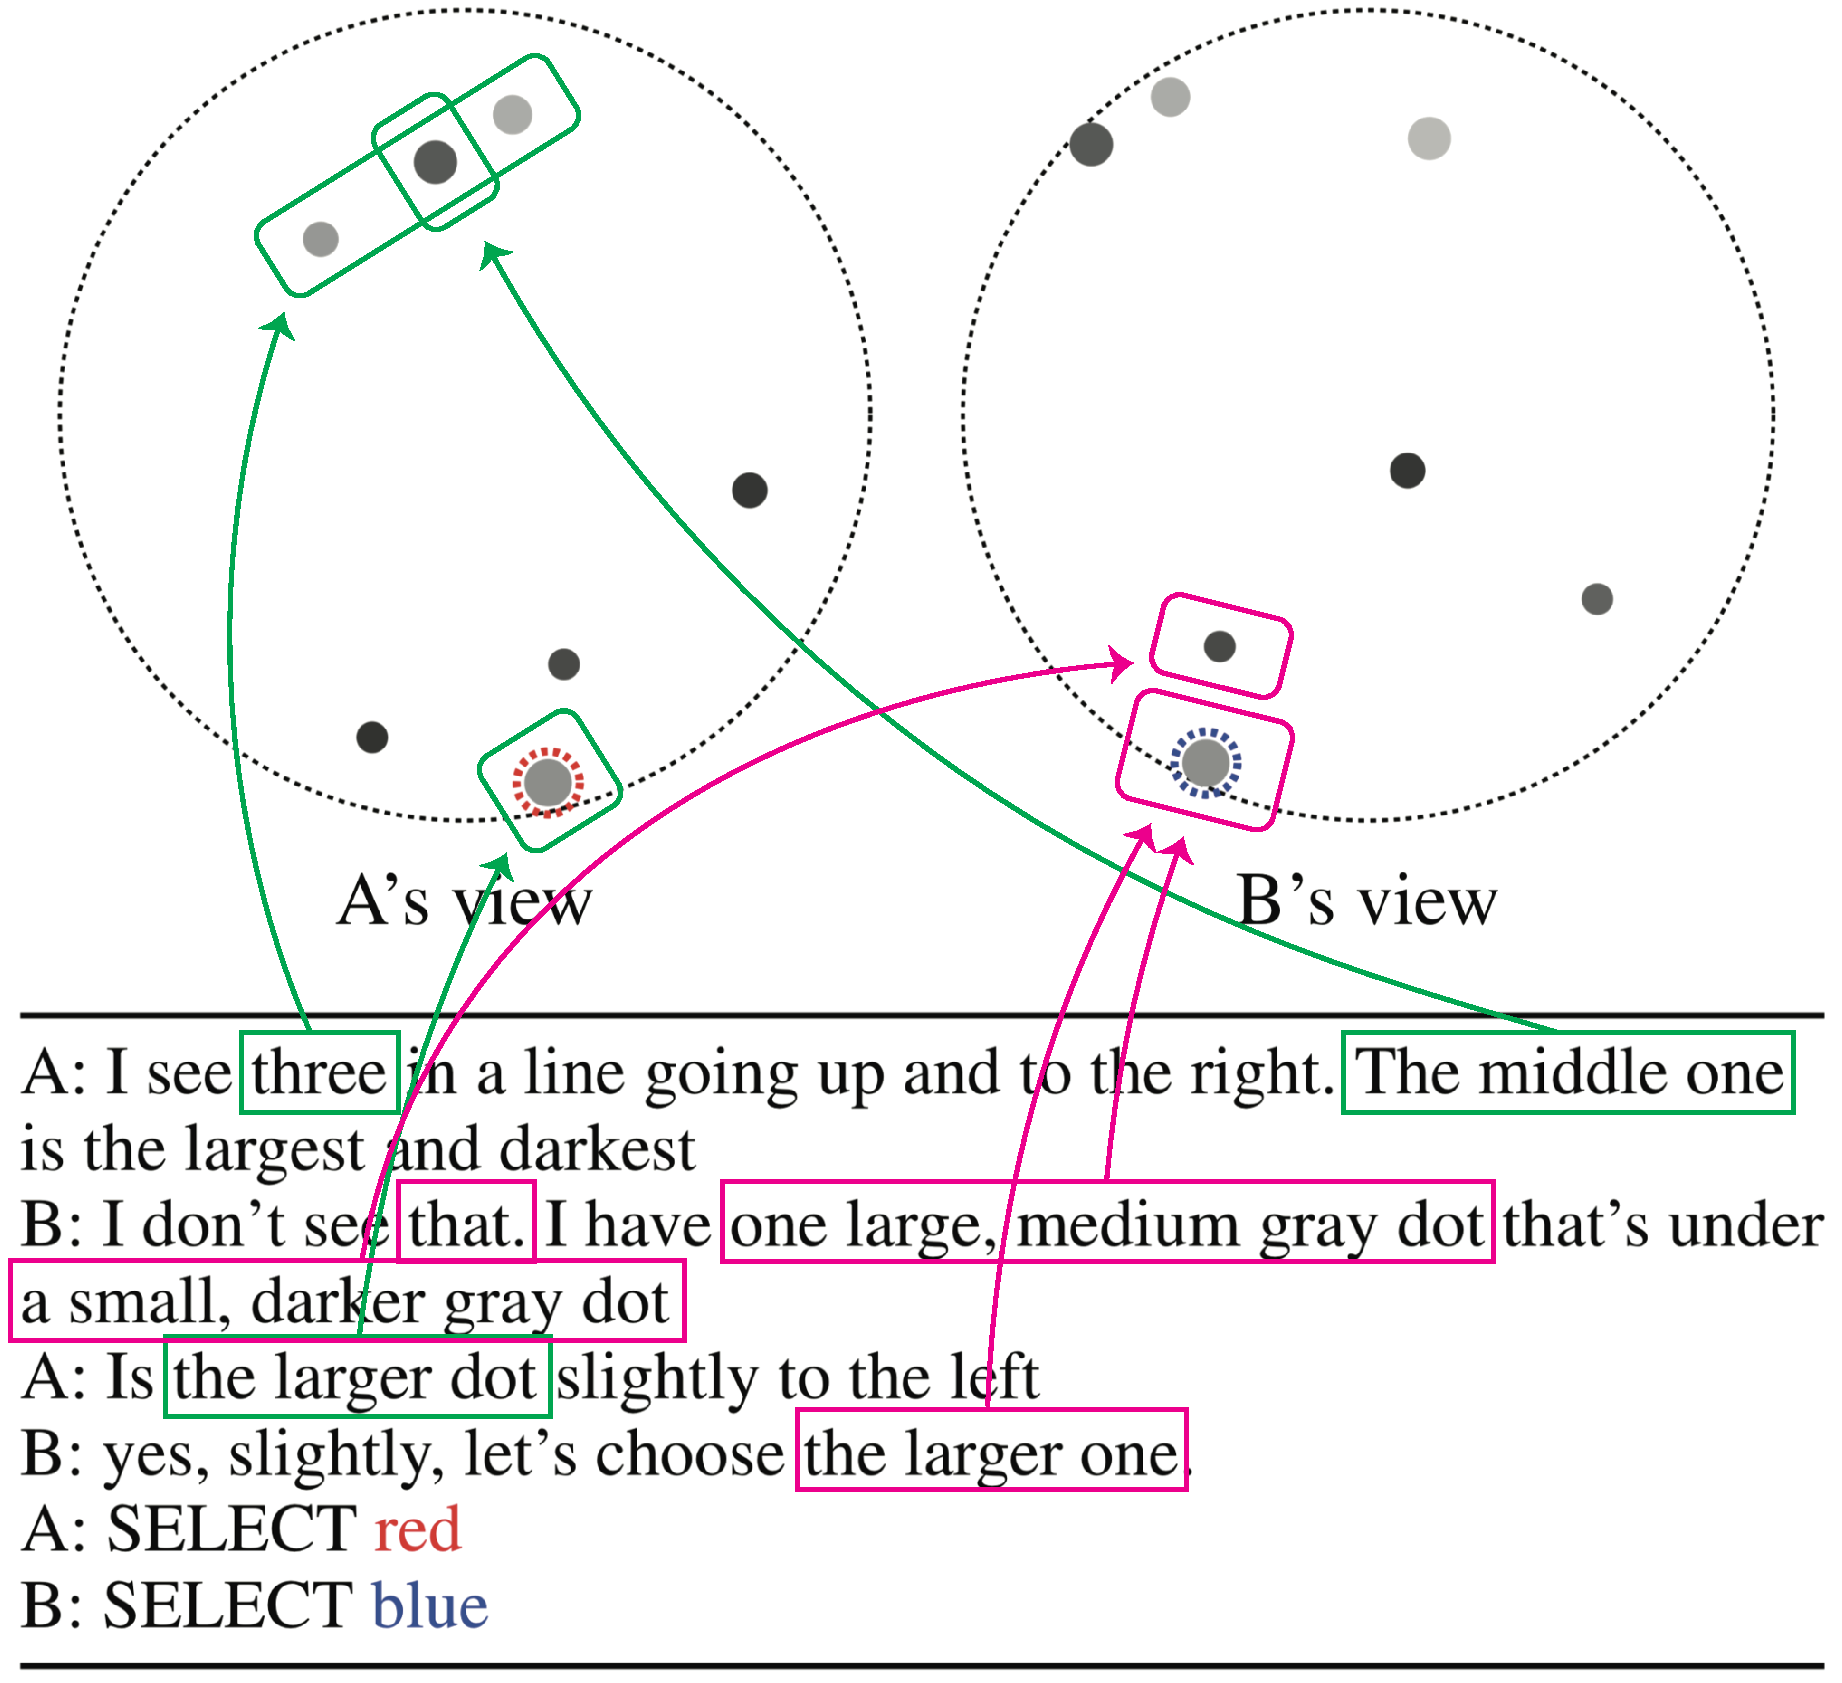
\includegraphics[width=0.7\textwidth]{annotated_dialogue.pdf}
\caption{A visualized example of our annotation. We identify all referring expressions in the dialogue and their intended referents based on the speaker's perspective (only one judgement shown in this example).
}
\label{04_fig:first_example}
\end{figure*}

Through our corpus analyses, we show that our annotation has high agreement in general but also includes a natural degree of reasonable disagreements, which verified that our annotation can be conducted reliably while capturing the ambiguity and uncertainty under continuous and partially-observable context. In addition, we give a more quantitative analysis of \textit{pragmatic expressions} as an illustrative example of analyses that can be conducted based on our annotation.

Finally, in our experiments, we show that our annotation is critical for interpreting and analyzing common grounding in baseline end-to-end dialogue systems, as well as improving their performance on difficult end tasks.

Overall, the contributions of this chapter are as follows:

\begin{itemize}
  \item We proposed a novel method of decomposing common grounding based on the central subtask of \textit{reference resolution} to study the intermediate process of common grounding.
  \item We conducted a large-scale annotation of 5,191 dialogues from OneCommon Corpus, including 40,172 referring expressions with multiple judgements for referent identification.
  \item We verified the \textit{reliability} of our annotation (while capturing genuine ambiguity based on reasonable disagreements) as well as the \textit{usefulness} for analyzing human common grounding strategies.
  \item Our experiments demonstrate that our annotation can be utilized for both interpreting and improving common grounding in end-to-end dialogue systems.
\end{itemize}

\section{Annotation Procedure}
\label{04_sec:annotation_procedure}

The goal of our annotation is to provide a \textit{general}, \textit{reliable} and \textit{useful} annotation of reference resolution to study the intermediate process of common grounding. In this work, we use the 5,191 dialogues in OneCommon Corpus which succeeded on the collaborative reference task, since they are expected to be of higher quality (c.f. Section \ref{03_subsec:results}). Our annotation procedure consists of two main steps: \textit{markable detection} to semi-automatically detect the referring expressions under consideration, followed by \textit{referent identification} to identify their referents.

As an optional step, we also conducted \textit{preprocessing} of the dialogues to correct obvious misspellings and grammatical errors. Due to the limited size of the vocabulary, we manually looked for rare unigrams and bigrams in the dialogue and carefully designed rules to correct them. Our preprocessing step is reversible, so the collected annotation can also be applied to the original dialogues without preprocessing.

\subsection{Step 1: Markable Detection}
\label{04_subsec:markable_detection}

In this study, we define a \textit{markable} to be an independent referring expression of the entities under consideration: in our case, the synthetic entities on the 2-D plane. Basically, we annotate a markable as a minimal noun phrase including all prenominal modifiers (such as determiners, quantifiers, and adjectives) but excluding all postnominal modifiers (such as prepositional phrases and relational clauses). This eliminates the complexity of the annotation because markables will not overlap or nest with each other.
%See the figures for many examples of the detected markables.

To reduce the annotation effort in the later process, we optionally annotate three attributes for each markable if they are obvious from the context: a \textit{generic} attribute when the markable is not specific enough to identify the referents, \textit{all-referents} when the markable is referring to all of the entities in the speaker's view, and \textit{no-referent} when the referents are empty. \textit{Generic} markables are ignored in our annotation, and the referents of \textit{all-referents} or \textit{no-referent} are annotated automatically in the later process. To reduce the redundancy of annotation, we consider a predicative noun phrase as a markable only if there is no previous markable in the same utterance that refers to the same entities: for example, ``\textit{a triangle}'' in ``\underline{three dots} are forming \textit{a triangle}'' is not considered as a markable since ``three dots'' is already annotated, but it is considered a markable in ``\underline{one light dot} and \underline{two dark dots} are forming \underline{\textit{a triangle}}'' (underlines indicate markables). We also annotate obvious \textit{anaphoric} and \textit{cataphoric} relations in the same utterance if they have identical referents: this way, the referents of anaphoric/cataphoric markables can be annotated automatically based on their antecedents/postcedents. However, we do not annotate such relations \textit{across utterances} as they can potentially refer to different entities, e.g. in the case of misunderstandings (as shown in Figure \ref{04_fig:misunderstanding_partial_understanding}).

The annotators were graduate students with sufficient experience and training, and we used the brat annotation tool \citep{stenetorp2012brat} to detect the markables, their attributes and relations. All available information were accessible during the annotation, including the original dialogues, players' observations and final selections.

\subsection{Step 2: Referent Identification}
\label{04_subsec:referent_identification}

Next, we used crowdsourcing on Amazon Mechanical Turk to collect large-scale judgements of the referents for each markable. Our visual interface for referent identification is shown in Figure \ref{04_fig:referent_identification_interface}. Annotators were instructed to read the instructions carefully, including the description of the underlying collaborative reference task. If the referents were ambiguous, they put a check on \textit{ambiguous} box and selected all possible candidate referents. If the referents were completely unidentifiable based on the available information, they put a check on \textit{unidentifiable} box (without selecting the referents).

To collect reliable annotations, we restriceted the workers to those with at least 100 previously completed HITs (submissions on AMT) and above 99\% acceptance rate. We paid the workers well, with \$0.25 for dialogues with less than 7 markables, \$0.35 with less than 14 markables, and \$0.45 otherwise. In addition, we automatically detected outlier submissions based on several statistics (such as the agreement with other workers) and manually reviewed them to encourage better work or reject clearly unacceptable works. The overall rejection rate was 1.18\%.

As a result of this careful crowdsourcing, we were able to collect a large-scale annotation of 103,894 judgements with at least 3 judgements for each of the 34,341 markables that required manual referent identification. As shown in Figure \ref{04_fig:misunderstanding_partial_understanding}, our annotation captures important phenomena of the intermediate process of common grounding (e.g. misunderstandings and partial understandings).

\begin{figure*}[tb!]
\centering \scalebox{0.9}{
\setlength\tabcolsep{12pt}
\begin{tabular}{cc}
	\raisebox{50pt}{\multirow{2}{*}{{\color{myred} \textbf{Misunderstanding}}}} & 
	\begin{tikzpicture}
	\node[inner sep=0pt] (agent_0) at (0,0)
	  {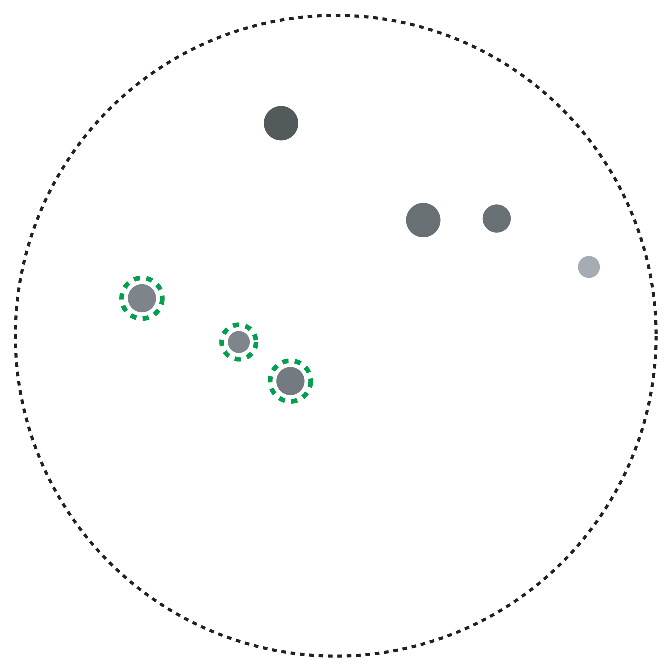
\includegraphics[width=0.31\columnwidth]{misunderstanding_A.pdf}};
	\node[inner sep=0pt] (agent_1) at (4.5,0)
	  {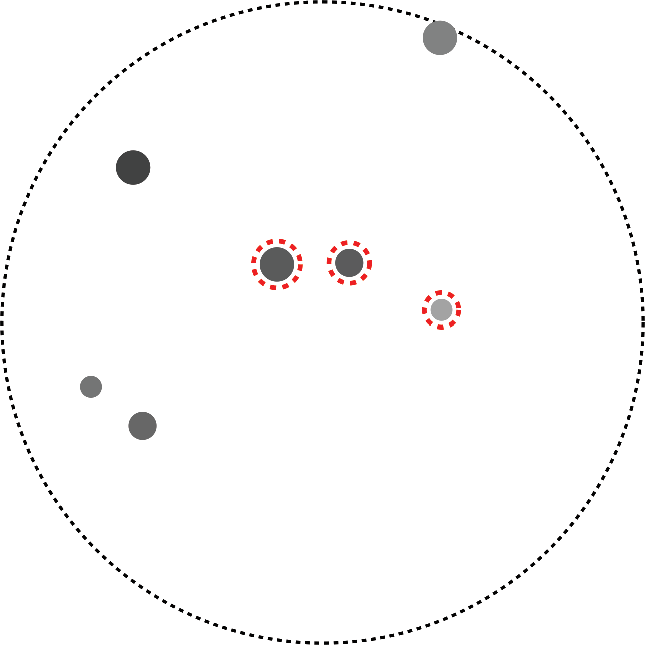
\includegraphics[width=0.31\columnwidth]{misunderstanding_B.pdf}};
	\node [below] at (0,-2.2) {A's View};
	\node [below] at (4.5,-2.2) {B's View};
	\end{tikzpicture} \\[-10pt]
	&
	\small
	\begin{tabular}[t]{@{}l@{}}
	\toprule
	A: I see {\color{mygreen} \underline{\textbf{three smaller circles}}} almost in a line slanting down\\
	from right to left \\
	B: I think I see {\color{myred} \underline{\textbf{it}}}.  Is \underline{the left one} the largest? ... \\
	\bottomrule
	\end{tabular}
	\vspace{6mm}\\
	\raisebox{50pt}{\multirow{2}{*}{{\color{myblue} \textbf{Partial Understanding}}}} & 
	\begin{tikzpicture}
	\node[inner sep=0pt] (agent_0) at (0,0)
	  {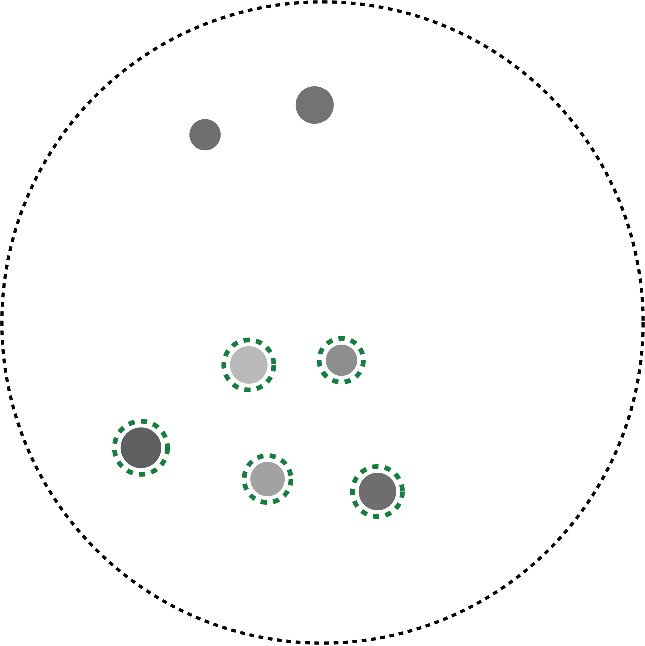
\includegraphics[width=0.31\columnwidth]{partial_understanding_A.pdf}};
	\node[inner sep=0pt] (agent_1) at (4.5,0)
	  {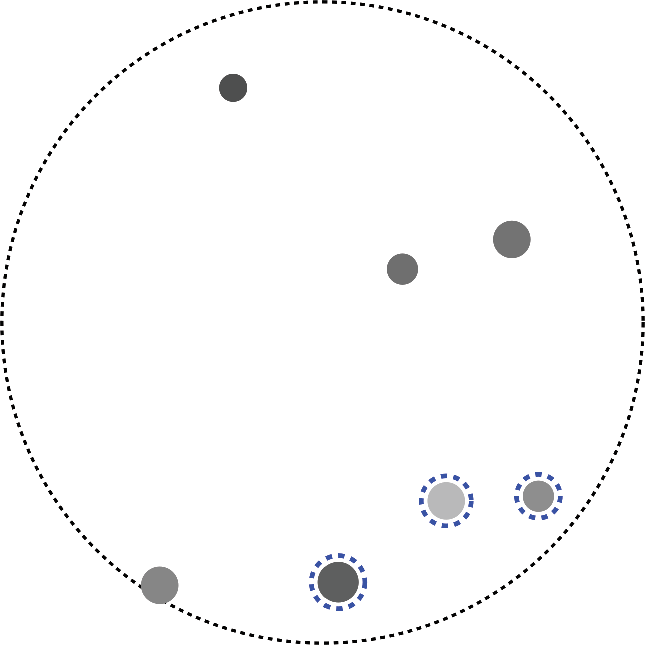
\includegraphics[width=0.31\columnwidth]{partial_understanding_B.pdf}};
	\node [below] at (0,-2.2) {A's View};
	\node [below] at (4.5,-2.2) {B's View};
	\end{tikzpicture} \\[-10pt]
	&
	\small
	\begin{tabular}[t]{@{}l@{}}
	\toprule
	A: I have  {\color{mygreen} \underline{\textbf{5 larger dots}}} close together, \underline{the bottom left one}\\
	is largest and darkest? \\
	B: i have {\color{myblue} \underline{\textbf{three}}} that could be part of that ... \\
	\bottomrule
	\end{tabular}
	\vspace{2mm}
\end{tabular}
}
\caption{Illustrative examples of misunderstanding and partial understanding captured by our annotation.}
\label{04_fig:misunderstanding_partial_understanding}
\end{figure*}

\begin{figure*}[tb!]
\centering
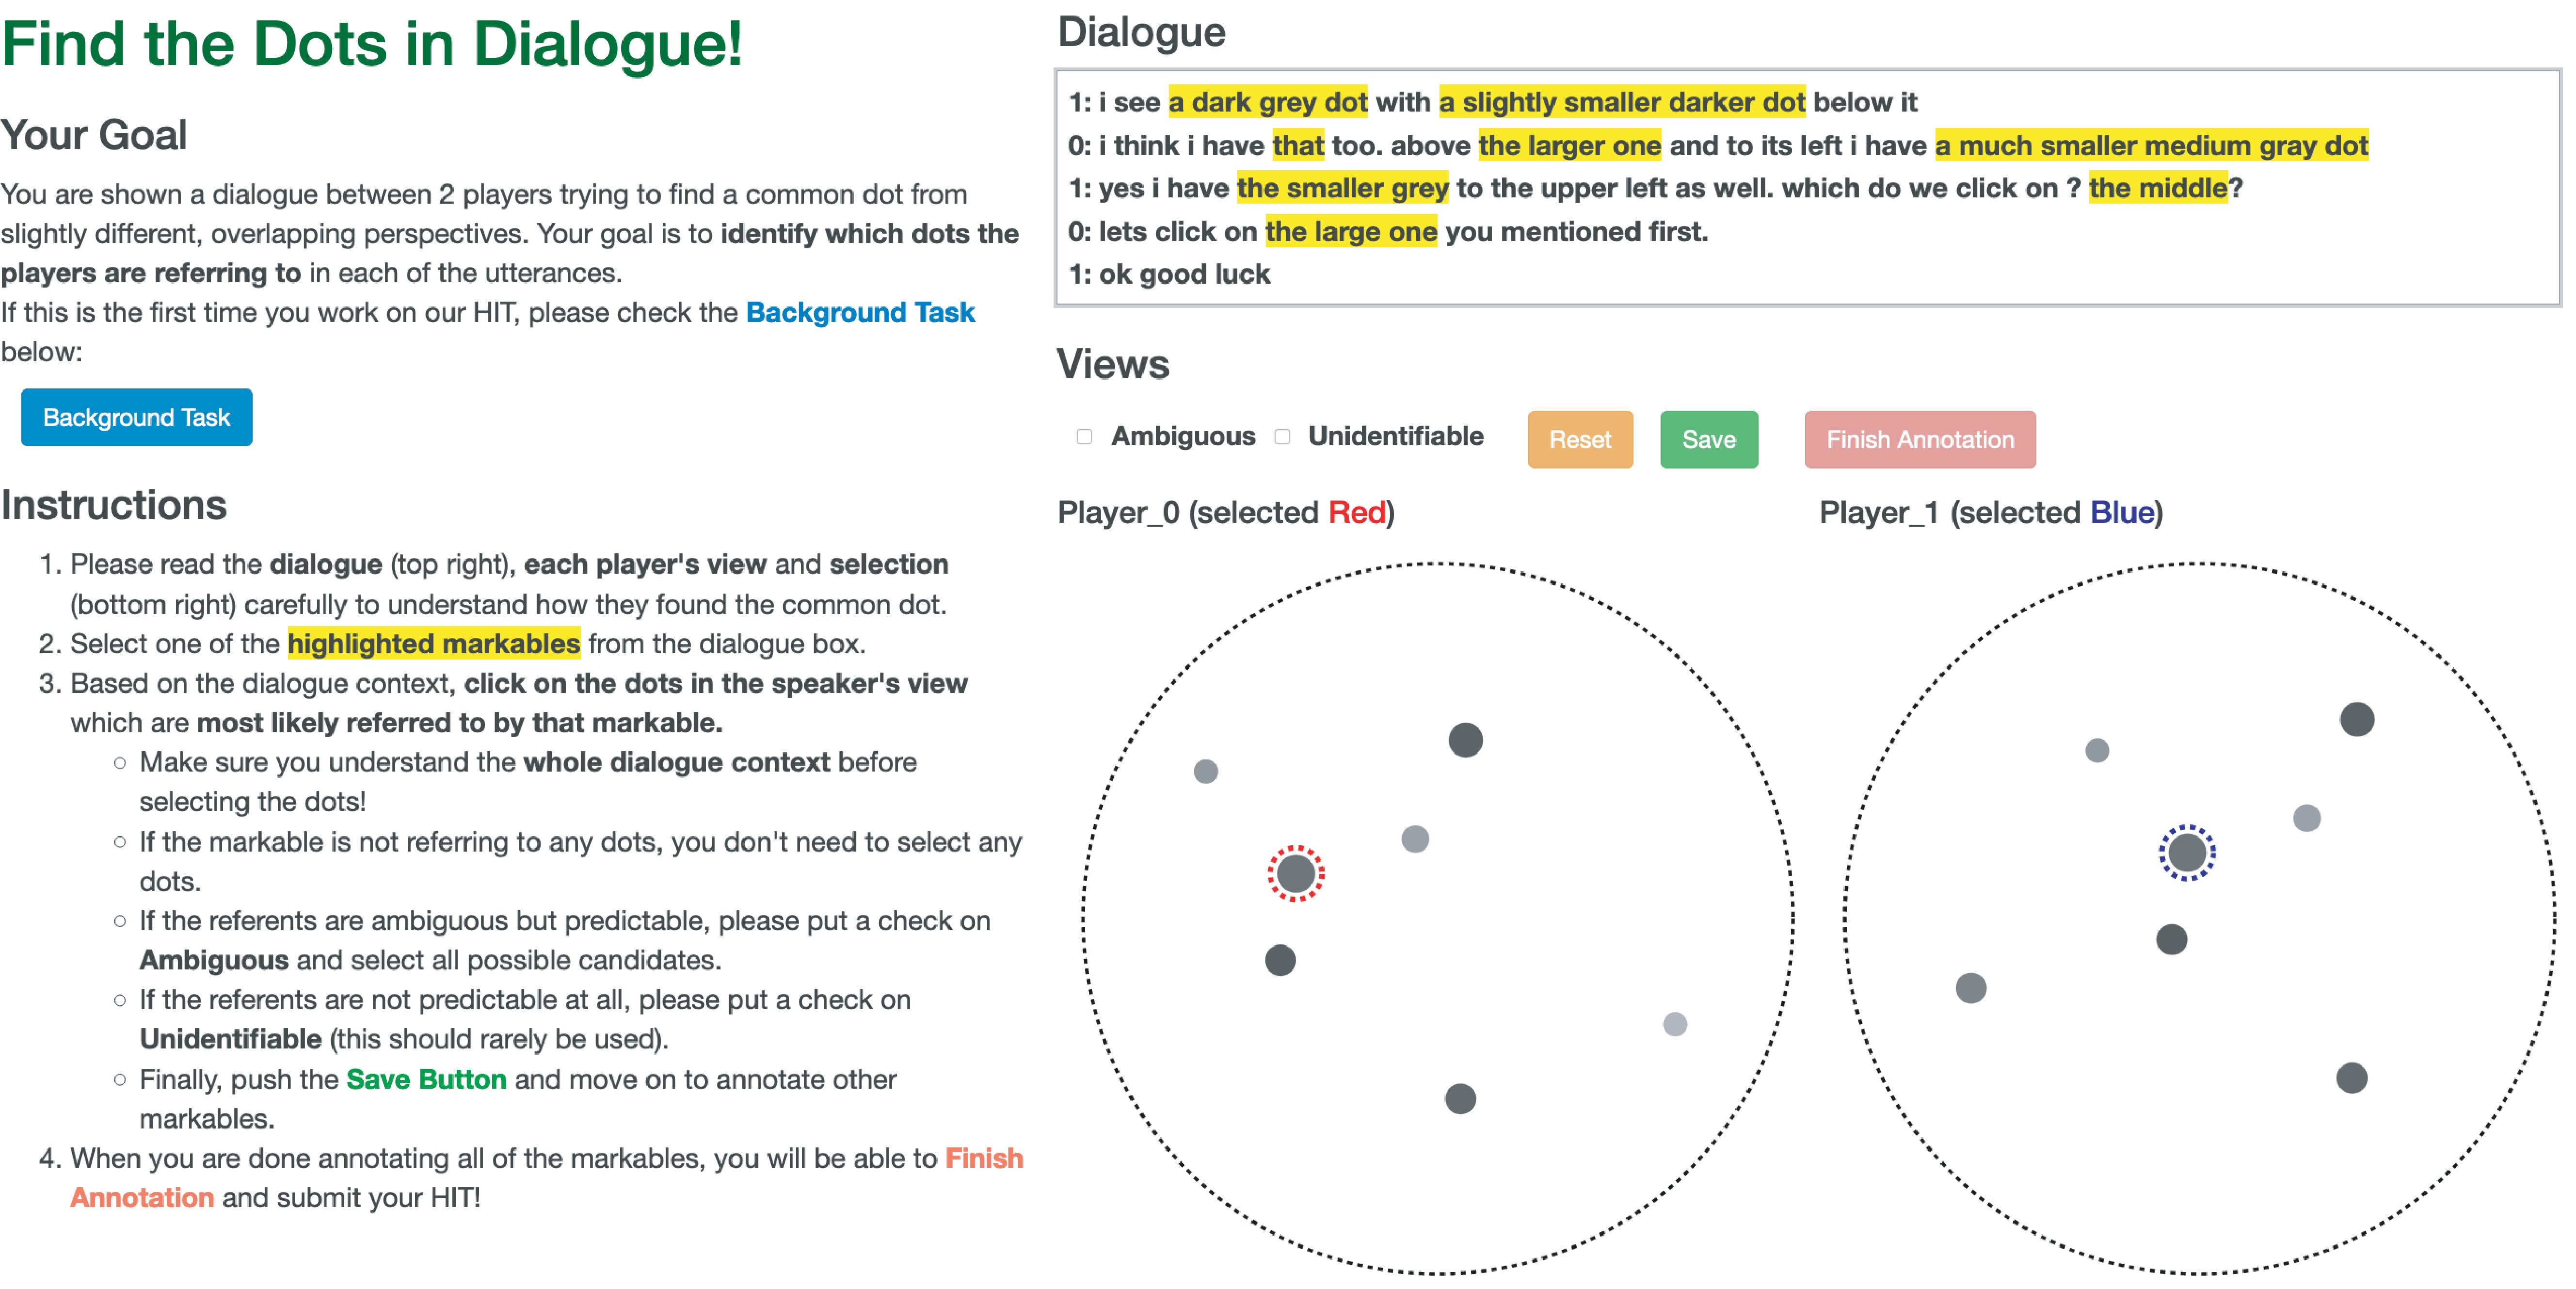
\includegraphics[width=\textwidth]{referent_identification.pdf}
\caption{Our visual interface used for referent identification.}
\label{04_fig:referent_identification_interface}
\end{figure*}


\section{Annotation Results}
\label{04_sec:annotated_corpus}

\subsection{Annotation Statistics}
\label{04_subsec:agreement_statistics}

First, we report the annotation statistics of markable detection in Table \ref{markable_detection_statsitics} and referent identification in Table \ref{04_tab:referent_identification_statistics}. All agreements are computed based on pairwise judgements, and we use Fleiss's Multi-$\pi$ \citep{fleiss1971measuring} to remove the effect of chance level agreements. For markable detection, agreement is calculated for the markable text span (start/end positions at the token level) based on 130 dialogues by 3 annotators. Agreements for markable attributes and relations were also reasonable, but we omit the results since they were optional and used only for the purpose of automatic referent identification. For referent identification, agreement is calculated at the entity-level (whether each entity is included in the referents) and the exact match rate at the markable-level (whether the set of referents match exactly).

Overall, we found high agreement for all annotations (including the crowdsourcing step), which verified the reliability of our annotation framework.

\begin{table*}[t!]
\centering \scalebox{0.78}{
\setlength\tabcolsep{5pt}
\begin{tabular}{ccccccc}
\toprule
\raisebox{-3pt}{\multirow{2}{*}{\# Markables}} & \raisebox{-3pt}{\multirow{2}{*}{\# All-Referents}} & \raisebox{-3pt}{\multirow{2}{*}{\# No-Referent}} & \raisebox{-3pt}{\multirow{2}{*}{\# Anaphora}} & \raisebox{-3pt}{\multirow{2}{*}{\# Cataphora}} & \multicolumn{2}{c}{Agreement (\%)} \\
\cmidrule{6-7}
 & & & & & Start Pos. & End Pos. \\
\midrule
40,172 & 128 & 1,149 & 4,548 & 6 & 99.11 (96.32) & 99.06 (96.11) \\
\bottomrule
\end{tabular}
}
\caption{\label{markable_detection_statsitics}
Annotation statistics for markable detection. Agreement is calculated at the token level (Fleiss's Multi-$\pi$ shown in parenthesis).
}
\end{table*}

\begin{table*}[t!]
\centering \scalebox{0.78}{
\begin{tabular}{cccccc}
\toprule
\# Markables & \# Judgements & Ambiguous (\%) & Unidentifiable (\%) & Agreement (\%) & Exact Match (\%)\\
\midrule
34,341 & 103,894 & 4.65 & 0.77 & 96.26 (88.66) & 86.90 \\
\bottomrule
\end{tabular}
}
\caption{\label{04_tab:referent_identification_statistics}
Annotation statistics for referent identification, along with the rate of \textit{ambiguous} and \textit{unidentifiable} checked in the judgements. Agreement is calculated at the entity-level (Fleiss's Multi-$\pi$ in parenthesis) and exact match rate at the markable-level.
}
\end{table*}

\subsection{Disagreement Analysis}
\label{04_subsec:disagreement_analysis}

\begin{figure}[th!]
\centering
\begin{tikzpicture}
\node[inner sep=0pt] (agent_0) at (0,0)
  {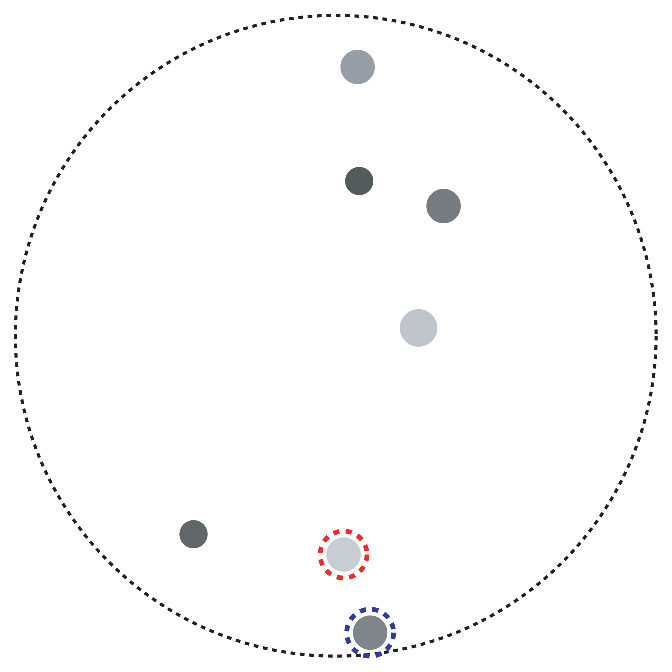
\includegraphics[width=0.3\textwidth]{disagreement_0.pdf}};
\node[inner sep=0pt] (agent_1) at (4.2,0)
  {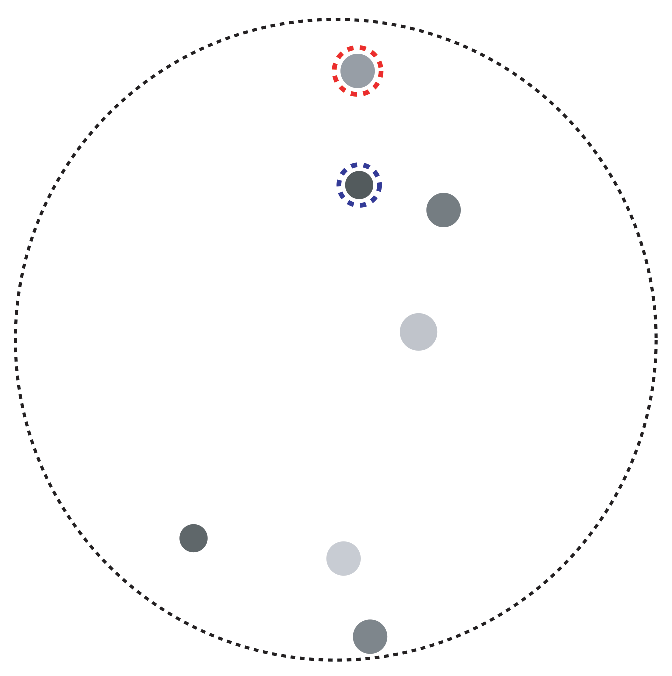
\includegraphics[width=0.3\textwidth]{disagreement_1.pdf}};
\node [below] at (0,3) {Annotator 1};
\node [below] at (4.2,3) {Annotator 2};
\node[text width=8cm] [below] at (2.1,-2.2) {{\color{myred} \underline{\textbf{medium sized light gray dot}}} with {\color{myblue} \underline{\textbf{a darker one}}} directly under {\color{myred} \underline{\textbf{it}}} and to the right? \\};
\end{tikzpicture}
\caption{An example of seemingly reasonable disagreement captured by our annotation.
}
\label{fig:reasonable_disagreement}
\end{figure}

However, it is natural that there is a certain degree of disagreement in referent interpretations. In fact, it is important to capture such disagreements as there can be genuine ambiguity and uncertainty under continuous and partially-observable context (see Figure \ref{fig:reasonable_disagreement} for an example). Therefore, in addition to \textit{explicitly} annotating the ambiguity and unidentifiability (as described in Section \ref{04_subsec:referent_identification}), we aim to capture them \textit{implicitly} by collecting multiple judgements from different annotators.

To study such disagreements in detail, we computed the agreement statistics (e.g. entity-level agreement) conditioned on \textit{the number of referents} in each judgement. To be specific, given a number of referents (from 0 to 7), we collected all judgements with that number of referents and computed the average pairwise agreements with all other judgements on the same markable. The results are summarized in Table \ref{num_referent_agreement}.

\begin{table}[t!]
\centering \scalebox{0.8}{
\setlength\tabcolsep{8pt}
\setlength{\aboverulesep}{0pt}
\setlength{\belowrulesep}{0pt}
\setlength{\extrarowheight}{.3ex}
\begin{tabular}{c|cc|c}
\toprule
\# Referents & Agreement (\%) & Exact Match (\%) & Judgements (\%) \\
\midrule
0 & 78.04 & 17.78 & \phantom{0}1.31 \\
1 & 97.45 & 90.28 & 71.81 \\
2 & 94.87 & 82.17 & 14.85 \\
3 & 93.93 & 83.03 & \phantom{0}7.51 \\
4 & 92.18 & 76.66 & \phantom{0}2.20 \\
5 & 90.31 & 71.03 & \phantom{0}0.88 \\
6 & 90.75 & 78.14 & \phantom{0}1.22 \\
7 & 81.47 & 62.50 & \phantom{0}0.21 \\
\bottomrule
\end{tabular}
}
\caption{\label{num_referent_agreement}
Agreement statistics conditioned on the number of referents (and the percentages of such judgements).
}
\end{table}

We can see that there is a significant amount of disagreements when the number of referents was judged to be 0 (none) or 7 (all). This could be due to several reasons: obvious cases were already annotated as \textit{no-referent} or \textit{all-referents} during markable detection (so only difficult cases were left), annotators simply made mistakes (e.g. forgot to annotate), or the referents were annotated as such when it was too difficult to identify them (e.g. all entities were potential referents). Since the number of such judgements were relatively small, their effect can be mitigated after appropriate aggregation of multiple judgements. We also expect that they provide a useful resource for studying disagreements caused by either the \textit{annotation error} or \textit{genuine ambiguity}, which is a critical problem when multiple interpretations are possible \citep{poesio-etal-2019-crowdsourced}.

In addition, we found that the exact match rate is the highest when the referent is only 1 and much lower as the number of referents increases. This is reasonable because referring expressions of multiple entities tend to be more pragmatic and ambiguous (e.g. \textit{``a cluster"}, \textit{``most of"}, \textit{``a line"}), and it would be more difficult to match the referents exactly. Note that entity-level agreements are still at a high level, and the interpreted referents seem to mostly overlap with each other.

Finally, to study which expressions tend to have higher (or lower) disagreements, we computed the correlations between the occurrence of common tokens (in the markable text) and the exact match rate (of the pairwise judements for the markable). Illustrative examples are shown in Table \ref{token_agreement_corrleation}.

\begin{table}[htb!]
\centering \scalebox{0.8}{
\setlength\tabcolsep{8pt}
\setlength{\aboverulesep}{0pt}
\setlength{\belowrulesep}{0pt}
\setlength{\extrarowheight}{.1ex}
\begin{tabular}{cc}
\begin{tabular}{c|cc}
\toprule
Low & $\rho$ & \# Count \\
\midrule
\textit{it} & -0.149 & 12.7K \\
\textit{any} & -0.103 & \phantom{0}0.5K \\
\textit{that} & -0.100 & 12.5K \\
\textit{your} & -0.083 & \phantom{0}1.5K \\
\textit{few} & -0.081 & \phantom{0}0.1K \\
\textit{what} & -0.081 & \phantom{0}0.4K \\
\textit{others} & -0.064 & \phantom{0}0.8K \\
\textit{line} & -0.062 & \phantom{0}1.7K \\
\textit{bunch} & -0.060 & \phantom{0}0.2K \\
\textit{all} & -0.048 & \phantom{0}1.1K \\
\textit{triangle} & -0.046 & \phantom{0}2.5K \\
\textit{some} & -0.042 & \phantom{0}0.2K \\
\textit{medium} & -0.041 & 12.5K \\
\textit{another} & -0.039 & \phantom{0}1.4K \\
\textit{and} & -0.029 & \phantom{0}1.7K \\
\bottomrule
\end{tabular}
&
\begin{tabular}{c|cc}
\toprule
High & $\rho$ & Count \\
\midrule
\textit{lower} & 0.028 & \phantom{0}1.3K \\
\textit{two} & 0.030 & 14.7K \\
\textit{three} & 0.031 & \phantom{0}4.2K \\
\textit{darkest} & 0.036 & \phantom{0}2.1K \\
\textit{larger} & 0.039 & \phantom{0}7.7K \\
\textit{middle} & 0.041 & \phantom{0}2.1K \\
\textit{smallest} & 0.043 & \phantom{0}2.0K \\
\textit{very} & 0.056 & \phantom{0}6.1K \\
\textit{top} & 0.061 & \phantom{0}5.2K \\
\textit{light} & 0.072 & 18.7K \\
\textit{tiny} & 0.076 & \phantom{0}7.8K \\
\textit{large} & 0.084 & 21.7K \\
\textit{the} & 0.125 & 55.0K \\
\textit{one} & 0.136 & 57.1K \\
\textit{black} & 0.145 & 26.9K \\
\bottomrule
\end{tabular}
\end{tabular}
}
\caption{\label{token_agreement_corrleation}
Tokens with low or high correlation with the exact match rate (Pearson's correlation coefficient shown in $\rho$).
}
\end{table}

In general, the correlations are very small and the amount of disagreements seem relatively constant across all token types. However, the general trend is still intuitive: ambiguous or complex expressions such as pronouns, interrogatives, quantifiers, and conjunctions tend to have negative correlations, while simple and plain expressions tend to have positive correlations.

To summarize the analysis, our annotation has high overall agreement but also includes interesting, reasonable disagreements which capture the ambiguity and uncertainty under continuous and partially-observable context.

\subsection{Pragmatic Expressions}
\label{04_subsec:pragmatic_expressions}

Finally, we give an illustrative example of additional analyses that can be conducted based on our annotation. To be specific, we give a more quantitative analysis of \textit{pragmatic expressions} which we introduced as a characteristic strategy under continuous context (Section \ref{03_subsec:difficulty_analysis}).

\begin{figure}[ht]
\centering
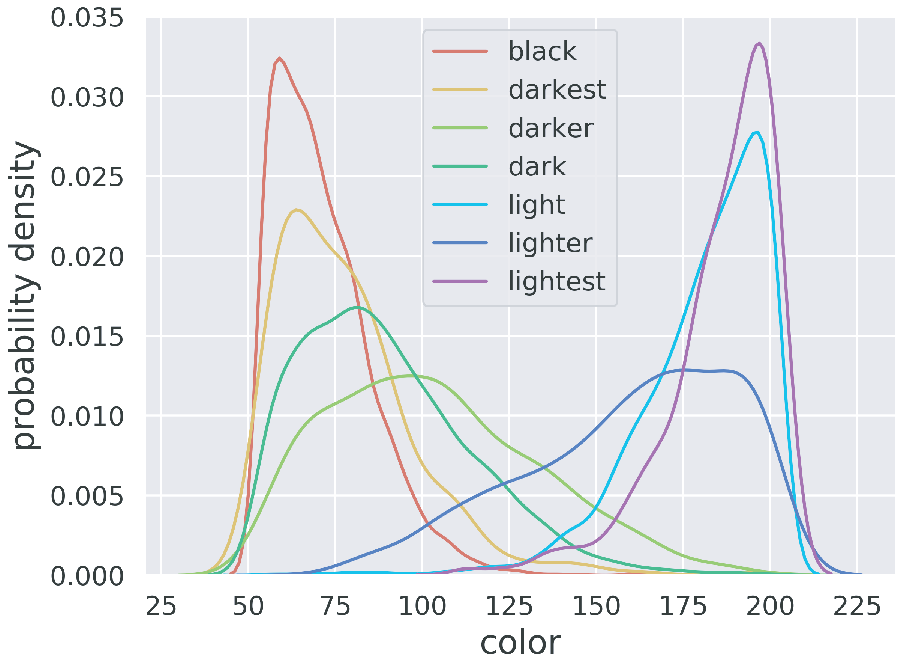
\includegraphics[width=0.7\textwidth]{color_distplot_cmyk.pdf}
\caption{Distributions of the actual color of the referents expressed by common adjectives (the range of color is 256 in grayscale, lower is darker).}
\label{fig:color_distplot}
\end{figure}

As an illustration, we focus on the pragmatic expressions of \textit{color} and estimate the distributions of the actual color of the referents described by the common adjectives. We simply assume that the adjective in the markable (minimal noun phrase) describes the color of the referents, since the exceptions (such as negation in the prenominal modifier) seemed rare and ignorable. For the sake of visualization, empirical distributions are smoothed based on kernel density estimation. As we can see in Figure \ref{fig:color_distplot}, all adjectives (including the specific color ``black'') have relatively wide distributions which overlap with each other. This is a strong evidence that the color expressions are pragmatic, i.e. the same adjective can be used for different colors (and in return, the same color can be described in different ways) depending on the context.


\section{Experiments}
\label{04_sec:experiments}

In this experiment, we evaluate and analyze baseline dialogue models based on the following three tasks: 

\begin{itemize}
  \item First is the \textbf{target selection task} from Chapter \ref{03_chp:task_formulation}, where the model predicts the target entity selected by each player at the end of collaborative reference. This task requires accurate recognition of the created common ground.
  \item Second is the \textbf{reference resolution task}, where the model predicts the referent entities for each markable in the dialogue. Note that the model is given only one player's observation and predicts the markables in that player's utterances only. This task requires accurate comprehension of the intermediate process of common grounding.
  \item Last is the \textbf{selfplay dialogue task}, where the model plays the whole collaborative reference task against an identical copy of itself. This requires the actual creation of common ground through natural language communication, despite against the copy of itself (and not with real humans).
\end{itemize}

To create the golden labels for reference resolution, we used simple majority voting based on the multiple judgements or automatically identified the referents based on markable attributes/relations. Note that markables were removed if the majority considered their referents as unidentifiable (in the referent identification step).

%If the referents were considered unidentifiable by the majority in step 2 (referent identification), we removed such markables from the dataset

%Note that markables were removed if the majority considered their referents as unidentifiable.

\subsection{Model Architecture}
\label{04_subsec:model_architecture}

\begin{figure*}[th]
\centering
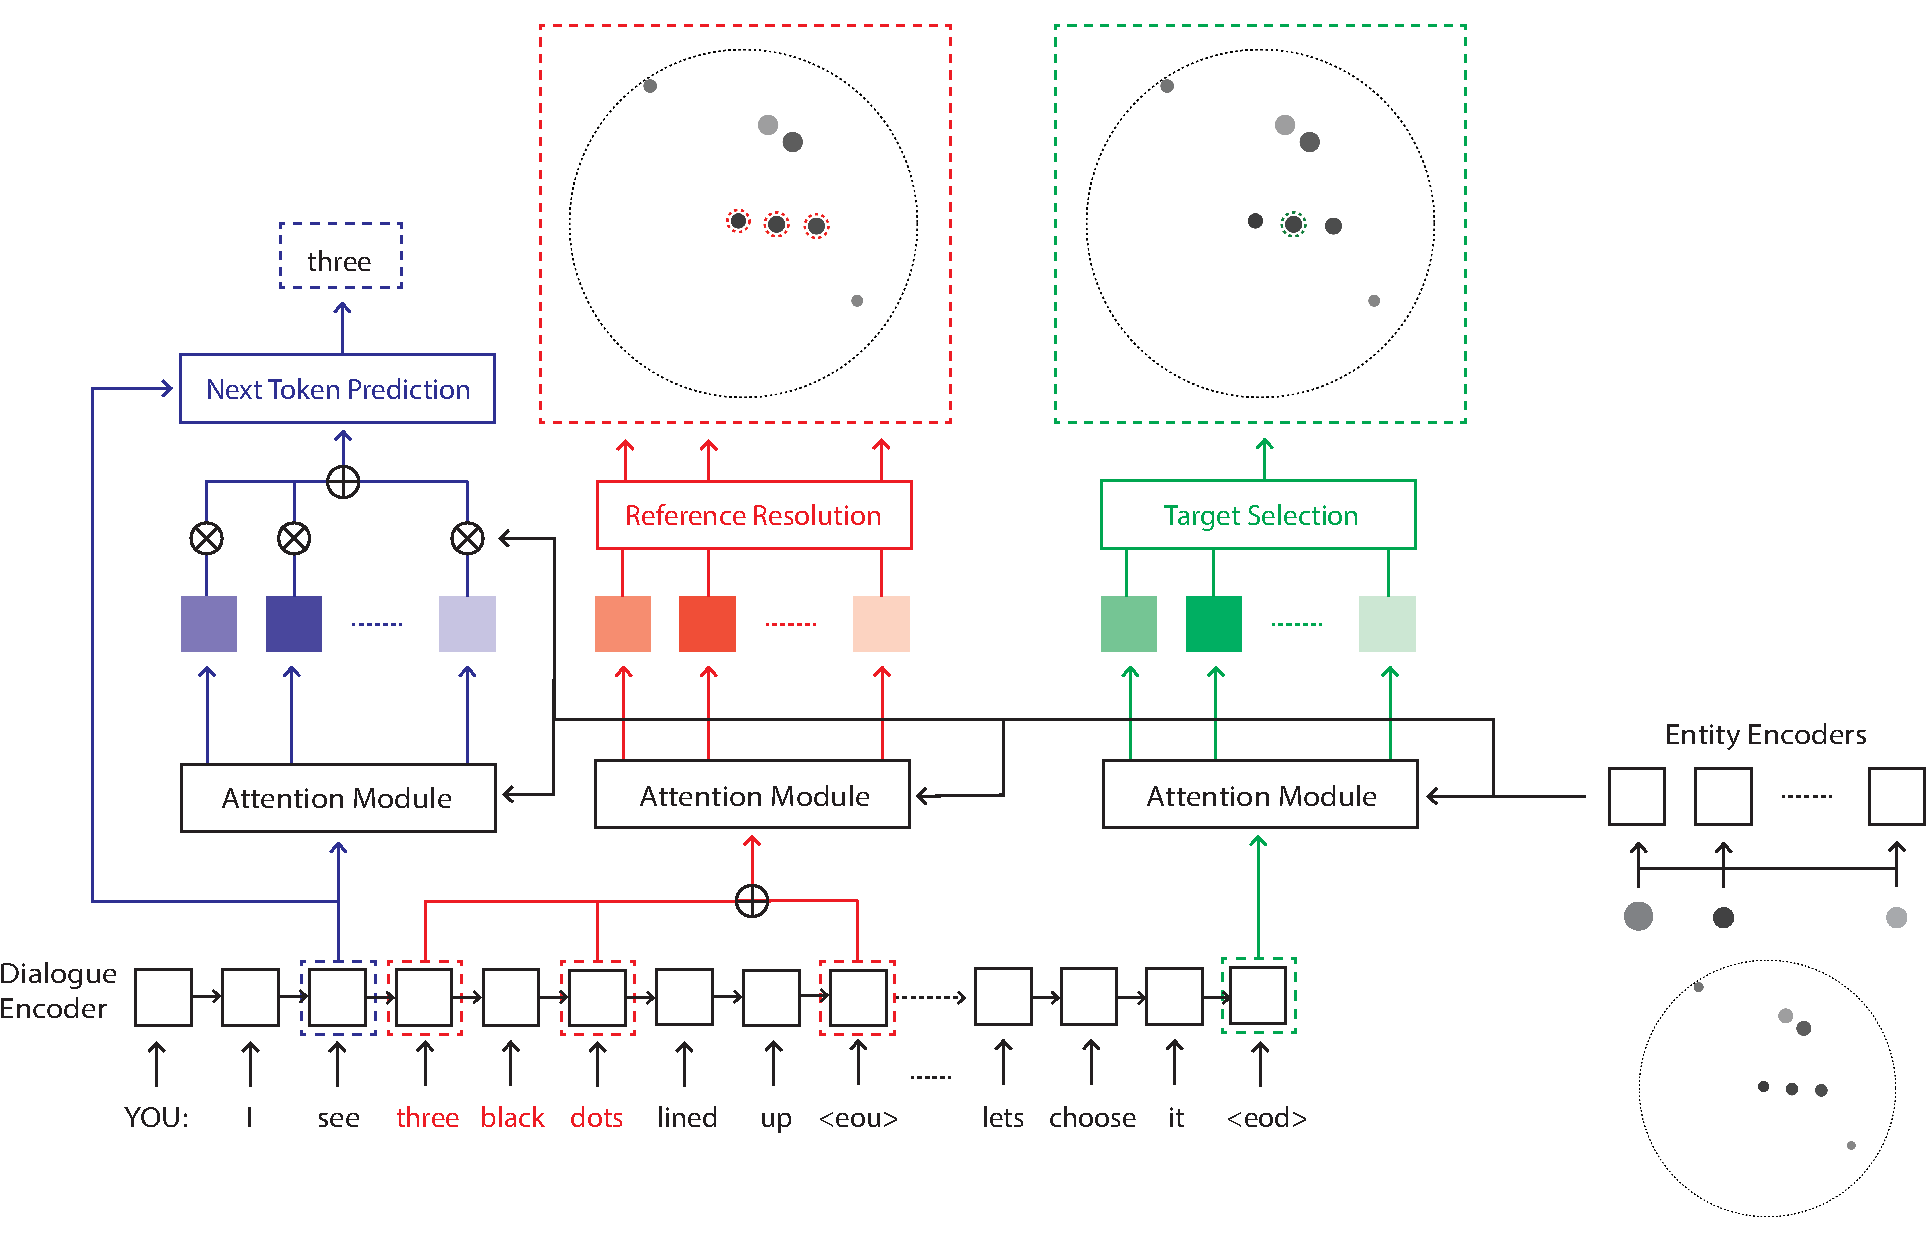
\includegraphics[width=\textwidth]{model_architecture.pdf}
\caption{Our baseline model architecture (best seen in color). TSEL decoder is shown in green, REF decoder and the input markable (``three black dots'') are in red, and DIAL decoder is in blue. All decoders share (some or all layers of) the attention module.}
\label{fig:model_architecture}
\end{figure*}

The overall architecture of our baseline end-to-end models is shown in Figure \ref{fig:model_architecture}.

\subsubsection{Encoders}

Our baseline models have two encoders: one for encoding dialogue tokens and one for context information.

Dialogue tokens are encoded based on a unidirectional GRU \citep{cho2014properties}. To encode context information, we use a shared \textit{entity encoder} to create entity-level representations of the context. This consists of two modules: an \textit{attribute encoder} which encodes the attributes of each entity (size, color and 2-D location) with a matrix followed by a tanh layer, and a \textit{relational encoder} which encodes relative attributes of each entity pairs with another matrix followed by a tanh layer. The final representation of each entity is the concatenation of its attribute encoding and the sum of relational encodings with the other 6 entities. Note that we refined the method from Chapter \ref{03_chp:task_formulation}, where the context is encoded into a single representation (and not entity-level representations).

%a \textit{relational encoder} which embeds pairs of entity attributes with another matrix followed by a tanh layer. The final embedding of each entity is the concatenation of its attribute embedding and the sum of relational embeddings with the other 6 entities.

\subsubsection{Decoders}

Our models can have up to three decoders: TSEL for target selection, REF for reference resolution, and DIAL for predicting next dialogue tokens. Each decoder shares (some or all layers of) the \textit{attention module} based on an MLP which computes a scalar score for each entity. Specifically, this module takes the representation of each entity and the following positions (states) of the GRU as the input: the \textit{final hidden state} for TSEL, the \textit{start/end positions of the markable} and the \textit{end position of the utterance} for REF, and the \textit{current hidden state} for DIAL. Based on the computed attention scores, TSEL simply computes the softmax and REF computes logistic regressions for each entity. DIAL reweights the entity representations based on their attention scores to focus on the relevant entities in next token prediction \citep{bahdanau2014nmt,xu2015show}.\\

In this experiment, we built five models based on different combinations of the three decoders. All models are trained with the same default hyperparameters, following the similar setup as Chapter \ref{03_chp:task_formulation}.


\subsection{Results}
\label{04_subsec:results}

\begin{table*}[tb!]
\centering \scalebox{0.77}{
\setlength\tabcolsep{6pt}
\setlength{\aboverulesep}{0pt}
\setlength{\belowrulesep}{0pt}
\setlength{\extrarowheight}{.3ex}
\begin{tabular}{c|cccccc}
\toprule
\multirow{2}{*}{Model} & \multirow{2}{*}{Target Selection} & Reference Resolution & \multicolumn{3}{c}{Selfplay Dialogue} \\
 & & (Accuracy / Exact Match) & \#Shared=4 & \#Shared=5 & \#Shared=6 \\
\midrule
TSEL & 67.79{\scriptsize $\pm$1.53}  & -  & - & - & - \\
REF & - & \textbf{85.75{\scriptsize $\pm$0.22}} / \textbf{33.91{\scriptsize $\pm$0.86}} & - & - & - \\
TSEL-REF & \textbf{69.01{\scriptsize $\pm$1.58}} & 85.47{\scriptsize $\pm$0.36} / 32.88{\scriptsize $\pm$1.28} & - & - & - \\
\midrule
TSEL-DIAL & 67.01{\scriptsize $\pm$1.29} & - & 42.07{\scriptsize $\pm$1.27} & 57.37{\scriptsize $\pm$1.29} & 77.00{\scriptsize $\pm$1.13} \\
TSEL-REF-DIAL & \textbf{69.09{\scriptsize $\pm$1.12}} & 85.86{\scriptsize $\pm$0.18} / 33.66{\scriptsize $\pm$0.93} & \textbf{45.78{\scriptsize $\pm$2.15}} & \textbf{61.95{\scriptsize $\pm$1.72}} & \textbf{80.01{\scriptsize $\pm$1.61}} \\
\midrule
Human & 90.79 & 96.26 / 86.90 & 65.83 & 76.96 & 87.00 \\
\bottomrule
\end{tabular}
}
\caption{\label{04_tab:baseline_results}
Results of our experiments. For reference resolution, \textit{accuracy} is computed at the entity-level and \textit{exact match rate} at the markable-level. Human scores are taken from Table \ref{03_tab:statistics} and \ref{04_tab:referent_identification_statistics} as a reference.
}
\end{table*}

We run the experiments 10 times with different random seeds and dataset splits. For selfplay dialogues, we generated 1,000 scenarios with each number of shared entities (4, 5 or 6) and set the output temperature to 0.25 during next token prediction. We report the mean and standard deviation of the results in Table \ref{04_tab:baseline_results}.

In terms of \textit{target selection} and \textit{selfplay dialogue} tasks, we found consistent improvements by training the models jointly with reference resolution (i.e. with REF decoder). This verified that even simple multi-task training with the central subtask can improve performance on difficult end tasks. The results for \textit{reference resolution} are reasonably high in terms of entity-level accuracy but much lower in terms of exact match rate. Considering the high agreements (Section \ref{04_subsec:agreement_statistics}) and improved reliability of the gold annotation after aggregation, we expect there to be a huge room for further improvements.

Overall, common grounding under continuous and partially-observable context is still a challenging task, and we expect our resource to be fundamental for solving this task along with the accurate capability of reference resolution.

\subsection{Further Analysis}
\label{subsection:analysis}

To demonstrate the advantages of our annotation for interpreting and analyzing dialogue systems, we give a more detailed analysis of TSEL-REF-DIAL model which performed well on all three tasks. In Table \ref{04_tab:exact_match_results}, we show the results for reference resolution grouped by the number of referents in the gold annotation. In terms of the exact match rate, we found that the model performs very well on 0 and 7 referents: this is because most of them can be recognized at the superficial level, such as ``\underline{none of them}", ``\underline{all of mine}", ``I don't have \underline{that}", etc. However, the model struggles on all other cases: the results are especially worse for markables with more than one referent. This shows that the model still lacks the ability of precisely tracking multiple referents, which can be expressed in complex, pragmatic ways (based on the grouping strategies).

In addition, we found that the correlation between the reference resolution accuracy (i.e. average accuracy of reference resolution in each dialogue) and the target selection accuracy (i.e. binary result of target selection in each dialogue) was relatively weak, with an average of only $0.23$ in the 10 runs of the experiments. This reveals that the model is often correct for the target selection task based on the \textit{wrong reason}, without tracking the referents correctly \citep{mccoy-etal-2019-right}. Our annotation is also useful for error analyses in recognizing common ground, e.g. by inspecting \textit{where} the model made a mistake and lost track of the correct referents.


\begin{table}[th]
\centering \scalebox{0.96}{
\small
\setlength\tabcolsep{8pt}
\setlength{\aboverulesep}{0pt}
\setlength{\belowrulesep}{0pt}
\setlength{\extrarowheight}{.3ex}
\begin{tabular}{c|cc|c}
\toprule
\# Referents & Accuracy (\%) & Exact Match (\%) & \# Count \\
\midrule
0 & 95.91{\scriptsize $\pm$1.38} & 83.53{\scriptsize $\pm$4.65}\phantom{0} & \phantom{0}148.5 \\
1 & 89.34{\scriptsize $\pm$0.17} & 36.86{\scriptsize $\pm$1.32}\phantom{0} & 2782.5 \\
2 & 78.14{\scriptsize $\pm$1.07} & 20.59{\scriptsize $\pm$1.90}\phantom{0} & \phantom{0}587.9 \\
3 & 70.64{\scriptsize $\pm$1.02} & 13.63{\scriptsize $\pm$2.06}\phantom{0} & \phantom{0}283.3 \\
4 & 69.12{\scriptsize $\pm$2.69} & 10.16{\scriptsize $\pm$3.47}\phantom{0} & \phantom{00}81.0 \\
5 & 73.57{\scriptsize $\pm$2.94} & 17.56{\scriptsize $\pm$5.88}\phantom{0} & \phantom{00}33.0 \\
6 & 78.69{\scriptsize $\pm$4.45} & 13.18{\scriptsize $\pm$7.31}\phantom{0} & \phantom{00}43.0 \\
7 & 74.60{\scriptsize $\pm$7.49} & 50.38{\scriptsize $\pm$11.40} & \phantom{00}22.3 \\
\bottomrule
\end{tabular}
}
\caption{\label{04_tab:exact_match_results}
Detailed results for the reference resolution task grouped by the number of referents in the gold annotation (along with the average counts in the test set).
}
\end{table}


\begin{figure}[th!]
\centering
\begin{tikzpicture}
\node[inner sep=0pt] (agent_0) at (0,0)
  {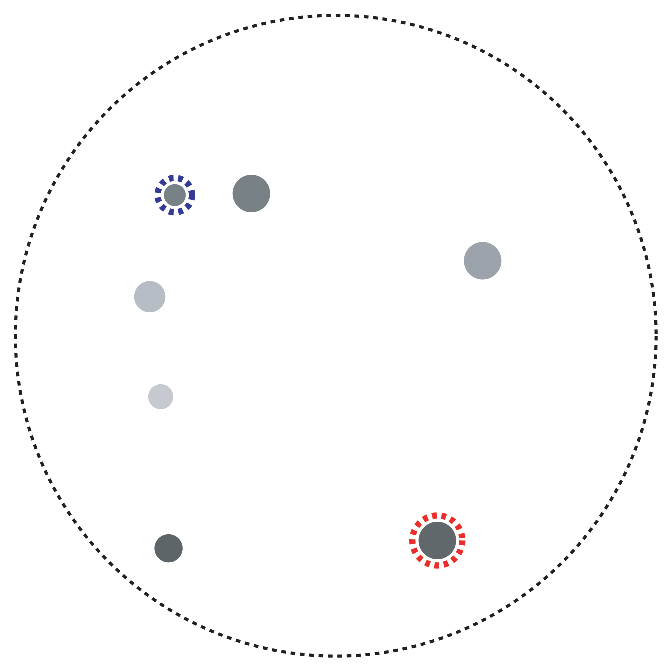
\includegraphics[width=0.3\textwidth]{selfplay_alice.pdf}};
\node[inner sep=0pt] (agent_1) at (4.2,0)
  {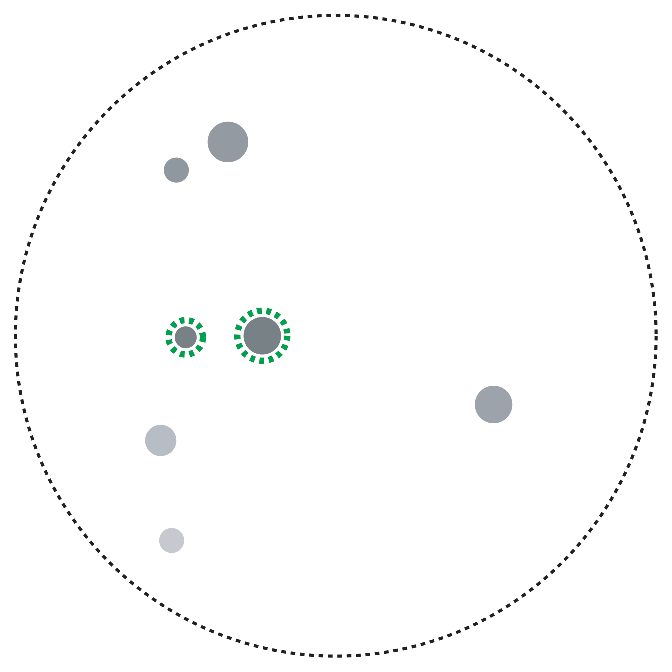
\includegraphics[width=0.3\textwidth]{selfplay_bob.pdf}};
\node [below] at (0,-2) {Model A's view};
\node [below] at (4.2,-2) {Model B's view};
\end{tikzpicture}
\small
\begin{tabular}{l}
\toprule
A: I have {\color{myred} \underline{\textbf{a large black dot}}} with {\color{myblue} \underline{\textbf{a smaller dark dot}}} to the\\ right of {\color{myred} \underline{\textbf{it}}} \\
B: I see {\color{mygreen} \underline{\textbf{that}}} . Let's pick \underline{the large black dot} \\
\bottomrule
\end{tabular}
\caption{An example dialogue from the selfplay dialogue task by the TSEL-REF-DIAL model. Predicted referents are highlighted (no referents are predicted for ``the large black dot'').
}
\label{fig:selfplay}
\end{figure}

Finally, we show an example dialogue from the selfplay task with the interpreted process of common grounding (Figure \ref{fig:selfplay}). Referring expressions are automatically detected by a BiLSTM-CRF tagger \citep{huang2015bidirectional} trained on our corpus with the result of 98.9\% accuracy at the token level. Based on the raw dialogue only, it is difficult to identify which entities model A is referring to. However, by visualizing the intended referents, we can see that model A is describing two entities in somewhat unnatural and inappropriate way (albeit using the anaphoric expression ``it'' appropriately). We can also verify that model B acknowledges this in a perfectly coherent way but without predicting any referent for ``the large black dot'': we often observed such phenomena, where the utterance by a model cannot be interpreted correctly \textit{even by itself}. Overall, our annotation allows for fine-grained analysis of both the \textit{capabilities} and \textit{incapabilities} of existing dialogue systems. The generated dialogue is short in this example, but our approach would be even more critical for interpretation as the dialogues get longer and more complicated.

\section{Related Work}
\label{03_sec:related_work}

Coreference and anaphora resolution have been studied extensively in NLP \citep{pradhan2011conll,poesio2016anaphora}, including disagreements in their interpretations \citep{recasens-etal-2012-annotating,poesio-etal-2019-crowdsourced}. The main novelty of our annotation schema is the focus on \textit{exophoric references} and direct annotation of the referents in the \textit{external modality}. This allows us to study the aspect of \textit{symbol grounding} in the visual context, as we discuss in the next chapter. This also enables reliable and intuitive annotation, even by using non-expert annotators for referent identifications. Finally, our annotation (at least indirectly) captures basic coreferences as well as complex associative anaphora (such as \textit{part-of} relations): with additional annotations, we can also capture more fine-grained, explicit relations between anaphora as well.

Our work is also relevant to the recent literature of interpretable and explainable machine learning \citep{doshi2017towards,lipton2016mythos}. Especially the analysis of neural based models is gaining attention in NLP \citep{belinkov-glass-2019-analysis}, including end-to-end dialogue models \citep{sankar-etal-2019-neural}. The main novelty of our approach is that we decompose the original task (\textit{common grounding}) based on its central subtask (or could be subtasks), define the subtask (\textit{reference resolution}) formally with an annotation framework, and create a large-scale resource to study the subtask along with the original task. Our approach has several advantages compared to previous analysis methods. First, it is applicable to \textit{both humans and machines}, which is especially important in dialogue domains where they interact. Second, it can be used to study the \textit{relationships} between the original task and its subtasks, which is critical for a more \textit{skill-oriented} evaluation of artificial intelligence \citep{Hernndez-Orallo:2017:MME:3110808,sugawara2017prerequisite}. Third, it can be used for investigating \textit{the dataset} on which the models are trained: this is important in many aspects, such as understanding undesirable biases in the dataset \citep{gururangan-etal-2018-annotation,sugawara-etal-2018-makes} or correct model predictions based on the \textit{wrong reasons} \citep{mccoy-etal-2019-right}. Finally, the collected resource can be used for both \textit{probing} whether the models solve the subtasks implicitly \citep{linzen2016assessing} or \textit{developing} new models which can be explicitly supervised, evaluated and interpreted based on the subtasks.

Finally, visually grounded dialogues have been studied in a wide variety of settings. In comparison, the main strengths and novelty of our (annotated) OneCommon Corpus can be summarized as follows:

\begin{enumerate}[label=(\Alph*)]
  \item Our corpus is based on the advanced setting of continuous and partially-observable context where complex common grounding strategies are introduced.
  \item Our corpus has the simplicity and controllability to make fully controlled experiments and analyses possible.
  \item Our corpus contains large-scale manual annotation of reference resolution and detailed analyses of agreements/disagreements based on multiple judgements.
\end{enumerate}

Prior work in common grounding \citep{potts2012goal,de2017guesswhat} and visual reference resolution \citep{tokunaga-etal-2012-rex,zarriess-etal-2016-pentoref} mostly focus on categorical or fully-observable settings and do not satisfy (A). While visual dialogues based on photographic scenes \citep{das2017visual,haber-etal-2019-photobook,ilinykh2019meetup} have the strengths of being more complex and realistic, they do not satisfy (B). \citet{gotze-boye-2016-spaceref} conducted a smaller-scale annotation of reference resolution but do not assess the reliability of the annotation, hence not satisfying (C). To the best of our knowledge, our work is the first (and only) resource to satisfy all of the above criteria.

\section{Conclusion}
\label{04_sec:conclusion}

One of the most influential models of common grounding to date is the \textit{contribution} model of \citet{clark1989contributing}: however, applying such theory in realistic settings can be difficult or even problematic. In this chapter, we proposed a novel method of decomposing common grounding based on the subtask of reference resolution to study the intermediate process of common grounding. Based on our annotated corpus, we demonstrated the advantages of our approach for analyzing human strategies as well as interpreting and improving baseline (end-to-end) dialogue models. Overall, we expect our study to be a fundamental step towards interpreting and improving common grounding through reference resolution.


\graphicspath{{05_analysis/figures/}} % Location of the graphics files

\chapter{Linguistic Analysis Based on Spatial Expressions}
\label{05_chp:analysis}

Recent models achieve promising results in visually grounded dialogues. However, existing datasets often contain undesirable biases and lack sophisticated linguistic analyses, which make it difficult to understand how well current models recognize their precise linguistic structures. To address this problem, we make two design choices: first, we focus on our OneCommon Corpus, which contains minimal bias by design. Second, we analyze their linguistic structures based on \textit{spatial expressions} and provide comprehensive and reliable annotation for 600 dialogues. We show that our annotation captures important linguistic structures including predicate-argument structure, modification and ellipsis. In our experiments, we assess our improved baseline's understanding of these structures through reference resolution (Chapter \ref{04_chp:interpretation}). We demonstrate that our annotation reveals both the strengths and weaknesses of our baseline in essential levels of detail. Overall, we propose a novel framework and resource for investigating fine-grained language understanding in visually grounded dialogues.

\section{Introduction}
\label{05_sec:introduction}

Visual dialogue is the task of holding natural, often goal-oriented conversation in a visual context \citep{das2017visual,de2017guesswhat}. This typically involves two types of advanced grounding: \textit{symbol grounding} \citep{harnad1990symbol}, which bridges symbolic natural language and continuous visual perception, and \textit{common grounding} \citep{clark1996using}, which refers to the process of developing mutual understandings through successive dialogues. As noted in \citet{monroe2017colors} and \citet{udagawa2019natural}, the \textit{continuous} nature of visual context introduces challenging symbol grounding of nuanced and pragmatic expressions. Some further incorporate \textit{partial observability} where the agents do not share the same context, which introduces complex misunderstandings and partial understandings that need to be resolved through advanced common grounding \citep{udagawa2019natural,haber-etal-2019-photobook}.

Despite the recent progress on these tasks, it remains unclear what types of linguistic structures can (or cannot) be properly recognized by existing models for two reasons. First, existing datasets often contain undesirable biases which make it possible to make correct predictions \textit{without} recognizing the precise linguistic structures \citep{goyal2017making,cirik-etal-2018-visual,agarwal-etal-2020-history}. Second, existing datasets severely lack in terms of sophisticated linguistic analysis, which makes it difficult to understand what types of linguistic structures exist or how they affect model performance.

To address this problem, we make the following design choices in this work:

\begin{itemize}%[leftmargin=1em] \setlength{\parskip}{0pt}
\item We focus on our OneCommon Corpus, a simple yet challenging collaborative reference task under continuous and partially-observable context. In this dataset, the visual contexts are kept simple and controllable to remove undesirable biases while enhancing linguistic variety. In total, 5,191 successful dialogues are fully annotated with referring expressions (called \textit{markables}) and their referents, which can be leveraged for further linguistic analysis.

\item To capture the linguistic structures in these dialogues, we propose to annotate \textit{spatial expressions} which play a central role in visually grounded dialogues. We take inspiration from the existing annotation frameworks \citep{pustejovsky2011iso,pustejovsky2011using,petruck-ellsworth-2018-representing,ulinski-etal-2019-spatialnet} but also make several simplifications and modifications to improve coverage, efficiency and reliability.\footnote{For instance, we define \textit{spatial expressions} in a broad sense and include spatial attributes (e.g. object size and color) as well as their comparisons.}
\end{itemize}

\begin{figure*}[t!]
\centering
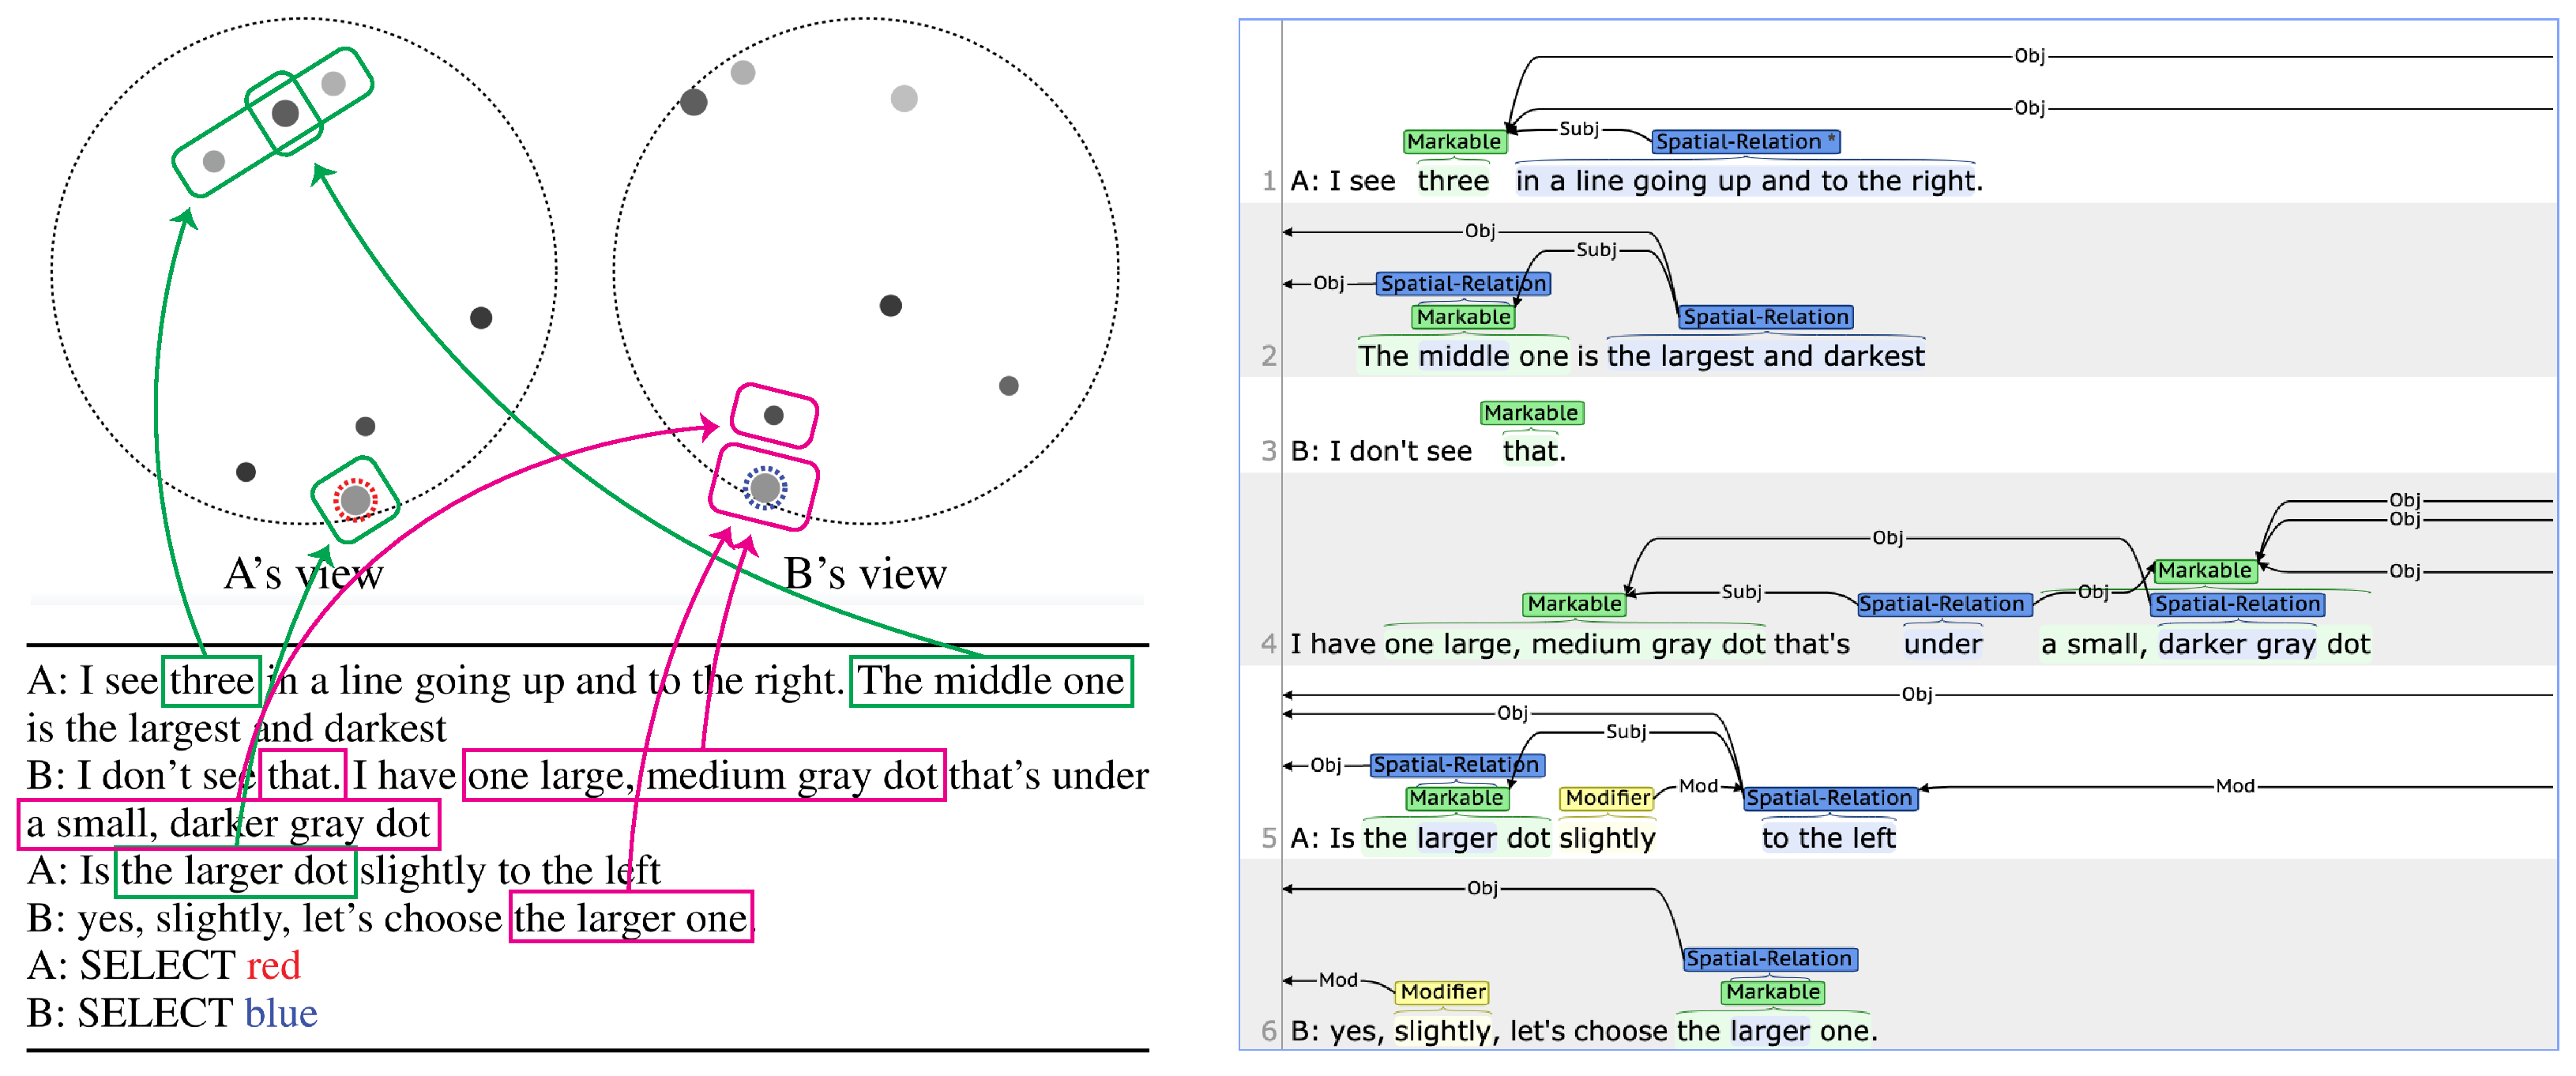
\includegraphics[width=\textwidth]{spatial_expression.pdf}
\caption{Example dialogue from OneCommon Corpus with reference resolution annotation (left) and our spatial expression annotation (right). We consider spatial expressions as predicates and annotate their arguments as well as modifiers.% For further details of the original dataset and our annotation schema, see Section \ref{sec:annotation}.
}
\label{05_fig:first_example}
\end{figure*}

As shown in Figure \ref{05_fig:first_example}, we consider spatial expressions as \textit{predicates} with existing markables as their \textit{arguments}. We distinguish the argument roles based on \textit{subjects} and \textit{objects}\footnote{Our \textit{subject}-\textit{object} distinction corresponds to other terminologies such as \textit{trajector}-\textit{landmark} or \textit{figure}-\textit{ground}.} and annotate \textit{modifications} based on nuanced expressions (such as ``slightly''). By allowing the arguments to be in previous utterances, our annotation also captures \textit{argument ellipsis} in a natural way.

In our experiments, we focus on reference resolution to study the model's comprehension of these linguistic structures. Since we found the existing baseline to perform relatively poorly (especially on the exact match rate), we propose a simple method of incorporating \textit{numerical constraints} in model predictions, which significantly improved its prediction quality.

Based on our annotation, we conduct a series of analyses to investigate whether the model predictions are \textit{consistent} with the spatial expressions. Our main finding is that the model is adept at recognizing entity-level attributes (such as color and size) but mostly fails in capturing inter-entity relations (especially placements): using the terminologies from \citet{landau1993and}, the model can recognize the \textit{what} but not the \textit{where} in spatial language. We also conduct further analyses to investigate the effect of other linguistic factors.

Overall, the contributions of this chapter are as follows:

\begin{itemize}
  \item We proposed a novel framework of annotating spatial expressions by leveraging referring expressions in visual dialogues.
  \item We sampled 600 random dialogues from OneCommon Corpus with reference resolution annotation (c.f. Chapter \ref{04_chp:interpretation}) and further conducted the annotation of spatial expressions.
  \item Our annotation captures important linguistic structures in visual dialogues, including predicate-argument structure, modification and ellipsis.
  \item Based on our improved baseline, we assess how well the end-to-end models can recognize the precise linguistic structures in the reference resolution task.
\end{itemize}


\section{Annotation Procedure}
\label{05_sec:annotation_procedure}

In this work, we randomly sample 600 dialogues from the annotated OneCommon Corpus (5,191 dialogues annotated with reference resolution) to conduct further annotation of spatial expressions. Our annotation procedure consists of three steps: \textit{spatial expression detection}, \textit{argument identification} and \textit{canonicalization}.
%Based on these annotation, we conduct fine-grained analyses of the dataset (Subsection \ref{subsec:annotation_results}) as well as the baseline models (Subsection \ref{subsec:model_analysis}). For further details and examples of our annotation, see Appendix \ref{sec:annotation_examples}.

\subsection{Step 1: Spatial Expression Detection}
\label{05_subsec:spatial_expression_detection}

Based on \citet{pustejovsky2011iso,pustejovsky2011using}, spatial expressions are defined as the ``constructions that make explicit reference to the spatial attributes of an object or spatial relations between objects''.\footnote{Note that their term \textit{object} corresponds to our term \textit{entity}.} We generally follow this definition and detect all spans of spatial attributes and relations in the dialogue. To make the distinction clear, we consider entity-level information (like color and size) as spatial attributes and other information (such as location and \textit{explicit} attribute comparison) as spatial relations. Spatial attributes could be annotated as adjectives (``dark''), prepositional phrases (``of light color'') or noun phrases (``a black dot''), while spatial relations could be adjectives (``lighter''), prepositions (``near''), and so on. We also detect the modification of spatial expressions based on negation and nuanced expressions, i.e. degree modifiers (c.f. Section \ref{03_subsec:difficulty_analysis}).

Although we allow certain flexibility in determining their spans, holistic/interdependent expressions (such as ``all shades of gray'', ``sloping up to the right'', ``very slightly'') were instructed to be annotated as a single span. Independent expressions (e.g. connected by conjunctions) could be annotated separately or jointly if they had the same structure (e.g. same arguments and modifiers).

For the sake of efficiency, we \underline{do not} annotate spatial attributes and their modifiers inside markables (see Figure \ref{05_fig:first_example}), since their spans and arguments are easy to be detected automatically.

\subsection{Step 2: Argument Identification}
\label{05_subsec:argument_identification}

Secondly, we consider the detected spatial expressions as \textit{predicates} and annotate referring expressions (markables) as their \textit{arguments}. This approach has several advantages: first, it has broad coverage since referring expressions are prevalent in visual dialogues. In addition, by leveraging \textit{exophoric} references which directly bridge natural language and the visual context, we can conduct essential analyses related to symbol grounding across the two modalities (c.f. Section \ref{02_sec:symbol_grounding}).

To be specific, we distinguish the argument roles based on subjects and objects. We allow arguments to be in previous utterances \textit{only if} they are unavailable in the present utterance. Multiple markables can be annotated for the subject/object roles, and no object need to be annotated in cases of spatial attributes, nominal/verbal expressions (``triangle'', ``clustered'') or \textit{implicit global objects} as in superlatives (``darkest (of all)''). If the arguments are indeterminable based on these roles (as in enumeration, e.g. ``\underline{From left to right}, there are ...''), they were marked as \textit{unannotatable}. Modificands of the modifiers (which could be either spatial attributes or relations) were also identified in this step. We show some illustrative examples in Figures \ref{05_fig:spatial_attribute}, \ref{05_fig:subject_ellipsis} and \ref{05_fig:unannotatable}.

\begin{figure}[t!]
\centering
\includegraphics[width=0.6\columnwidth]{C_09b2a91332a64c12a3235d69a9e1f5da.pdf}
\caption{An example with spatial attributes (e.g. ``small and light'').}
\label{05_fig:spatial_attribute}
\end{figure}

\begin{figure}[t!]
\centering
\includegraphics[width=0.6\columnwidth]{C_3bc6ee0e230445ab98661b03f6903ae5.pdf}
\caption{An example with subject ellipsis (``B: smaller?'').}
\label{05_fig:subject_ellipsis}
\end{figure}

\begin{figure}[t!]
\centering
\includegraphics[width=0.6\columnwidth]{C_0e7e8399d1b64b598bcafa58976c05ac.pdf}
\caption{An example with unannotatable relation, ``going (small medium large)''.}
\label{05_fig:unannotatable}
\end{figure}

\subsection{Step 3: Canonicalization}
\label{05_subsec:canonicalization}

Finally, we conduct canonicalization of the spatial expressions and modifiers. Since developing a complete ontology for this domain is infeasible or too expensive, we focus on canonicalizing the central \textit{spatial relations} in this work: we \underline{do not} canonicalize spatial attributes manually since this can be conducted automatically (c.f. Section \ref{05_subsec:spatial_attributes}).

According to \citet{landau2017update}, there are 2 classes of relations in spatial language: \textit{functional} class whose core meanings engage force-dynamic relationship (such as \textit{on}, \textit{in}) and \textit{geometric} class whose core meanings engage geometry (such as \textit{left}, \textit{above}). Since functional relations are less common in this dataset and more difficult to define due to their vagueness and context dependence \citep{platonov2018computational}, we focus on the following 5 categories of geometric relations and attribute comparisons, including a total of 24 canonical relations which can be defined explicitly.

\begin{itemize}

\item \textbf{Direction} requires the subjects and objects to be placed in a certain orientation: \textit{left}, \textit{right}, \textit{above}, \textit{below}, \textit{horizontal}, \textit{vertical}, \textit{diagonal}.

\item \textbf{Proximity} is related to the distance between subjects, objects or other entities: \textit{near}, \textit{far}, \textit{alone}.

\item \textbf{Region} restricts the subjects to be in a certain region determined by the objects: \textit{interior}, \textit{exterior}.

\item \textbf{Color comparison} is related to the comparison of color among subjects and objects: \textit{lighter}, \textit{lightest}, \textit{darker}, \textit{darkest}, \textit{same color}, \textit{different color}.

\item \textbf{Size comparison} is related to the comparison of size among subjects and objects: \textit{smaller}, \textit{smallest}, \textit{larger}, \textit{largest}, \textit{same size}, \textit{different size}.

\end{itemize}

To be specific, we annotate whether each detected spatial relation \textit{implies} any of the 24 canonical relations. Each spatial relation can imply multiple canonical relations (e.g. ``on the upper right'' implies \textit{right} and \textit{above}) or none (e.g. ``(forming a) triangle'' does not imply any of the above relations).

In addition, we consider 6 modification types (the 5 degree modifiers from Figure \ref{03_fig:degree_modifiers} and \textit{negation}) and canonicalize each modifier into one type. For example, ``very slightly'' is considered to have the overall type of the \textit{diminisher}.


\section{Annotation Results}
\label{05_sec:annotation_results}

\subsection{Annotation Reliability}
\label{05_subsec:annotation_reliability}

\begin{table}[ht]
\centering \small
\setlength{\tabcolsep}{9pt}
\setlength{\aboverulesep}{0pt}
\setlength{\belowrulesep}{0pt}
\setlength{\extrarowheight}{.75ex}
\begin{tabular}{ll|cc}
\toprule
\multicolumn{2}{c|}{Annotation} & Agreement (\%) & Cohen's $\kappa$ \\
\midrule
\multirow{3}{*}{Span Detection} & Attribute & 98.5 & 0.88 \\
& Relation & 95.1 & 0.87 \\
& Modifier & 99.2 & 0.86 \\
\midrule
\multirow{3}{*}{\parbox{2cm}{Argument Identification}} & Subject & 98.8 & 0.96 \\
& Object & 95.9 & 0.79 \\
& Modificand & 99.6 & 0.98 \\
\midrule
\multirow{2}{*}{Canonicalization} & Relation & 99.7 & 0.96 \\
& Modifier & 87.5 & 0.83 \\
\bottomrule
\end{tabular}
\caption{
Results of our reliability analysis.
}
\label{05_tab:reliability_results}
\end{table}

To test the reliability of our annotation, two trained annotators (the authors) independently detected the spatial expressions and modifiers in 50 dialogues. Then, using the 50 dialogues from one of the annotators, two annotators independently conducted argument identification and canonicalization. We show the observed agreement and Cohen's $\kappa$ \citep{cohen1968weighted} in Table \ref{05_tab:reliability_results}.

For span detection, we computed the token level agreement of spatial expressions and modifiers. Despite having certain freedom for determining their spans, we observed high agreement in general (including their start/end positions).

For argument identification, we computed the exact match rate of the arguments and modificands. As a result, we observed near perfect agreement for subject/modificand identification. For object identification, the result was comparatively worse: however, upon further inspection, we verified that 73.5\% of the disagreements were essentially based on the same markables (e.g. coreferences).

Finally, we observed reasonably high agreement for relation/modifier canonicalization as well. Overall, we conclude that all steps of our annotation can be conducted with high reliability.

\subsection{Annotation Statistics}
\label{05_subsec:annotation_statistics}

\begin{table}[th]
\centering \small
\setlength{\tabcolsep}{9pt}
\begin{tabular}{lcc}
\toprule
 & Attribute & Relation \\
 \midrule
Total annotated & 378 & 4,300 \\
Average per dialogue & 0.63 & 7.17 \\
Unique expressions & 121 & 1,139 \\
Inter-utterance subject (\%) & 1.59 & 1.37 \\
Inter-utterance object (\%) & - & 14.65 \\
No object (\%) & - & 30.84 \\
Unannotatable (\%) & 0.79 & 0.79 \\
\midrule
Modified (\%) & 36.51 & 16.86 \\
\phantom{----}-- Diminisher & 1.06 & 8.12 \\
\phantom{----}-- Moderator & 19.31 & 0.67 \\
\phantom{----}-- Booster & 9.00 & 2.16 \\
\phantom{----}-- Approximator & 7.41 & 4.26 \\
\phantom{----}-- Maximizer & 0.27 & 1.40 \\
\phantom{----}-- Negation & 0.53 & 0.42 \\
\bottomrule
\end{tabular}
\caption{
Statistics of our spatial expression annotation in 600 random dialogues.
}
\label{05_tab:annotation_statistics}
\end{table}

The basic statistics of our annotation are summarized in Table \ref{05_tab:annotation_statistics}. Note that there are relatively few spatial attributes annotated, since most of them appeared inside the markables (hence not detected manually). However, a large number of spatial relations with non-obvious structures were identified.

In both expressions, we found over 1\% of the subjects and 14\% of the objects to be present only in previous utterances, which indicates that argument level ellipses are common and need to be resolved in visual dialogues. For spatial relations, about 30\% did not have any explicit objects.

Our annotation also verified that a large portion of the spatial expressions (37\% for spatial attributes and 17\% for relations) accompanied modifiers. In addition, we can see that \textit{neutrality} is the most common type of modification for spatial attributes (as in \textit{medium gray}, \textit{medium sized}), and \textit{subtlety} and \textit{uncertainty} to be the most common types for spatial relations. It is interesting to note that the frequencies of modification types vary significantly with spatial attributes and relations, except for \textit{negation}.

Finally, less than 1\% of spatial expressions were \textit{unannotatable} based on our schema, which verifies its broad coverage. Overall, our annotation can capture important linguistic structures of visually grounded dialogues, and it is straightforward to conduct even further analyses (e.g. by focusing on specific canonical relations or modifications).

\section{Model Refinement}
\label{05_sec:model_evaluation}


\subsection{Evaluation}
\label{05_subsec:evaluation}

In our experiments, we focus on the \textit{reference resolution task} in OneCommon Corpus. As we discussed in Chapter \ref{04_chp:interpretation}, this can be used for probing the model's understanding of the intermediate dialogue process. As illustrated in Figure \ref{05_fig:first_example} (left), the goal of the task is to predict the referents of each markable based on the \textit{speaker}'s perspective. To collect model predictions for all dialogues, we split the whole dataset into 10 equal-sized bins and use each bin as the test set in the 10 rounds of the experiments.

\subsection{Model Architecture}
\label{05_subsec:models}

\begin{figure}[ht]
\centering
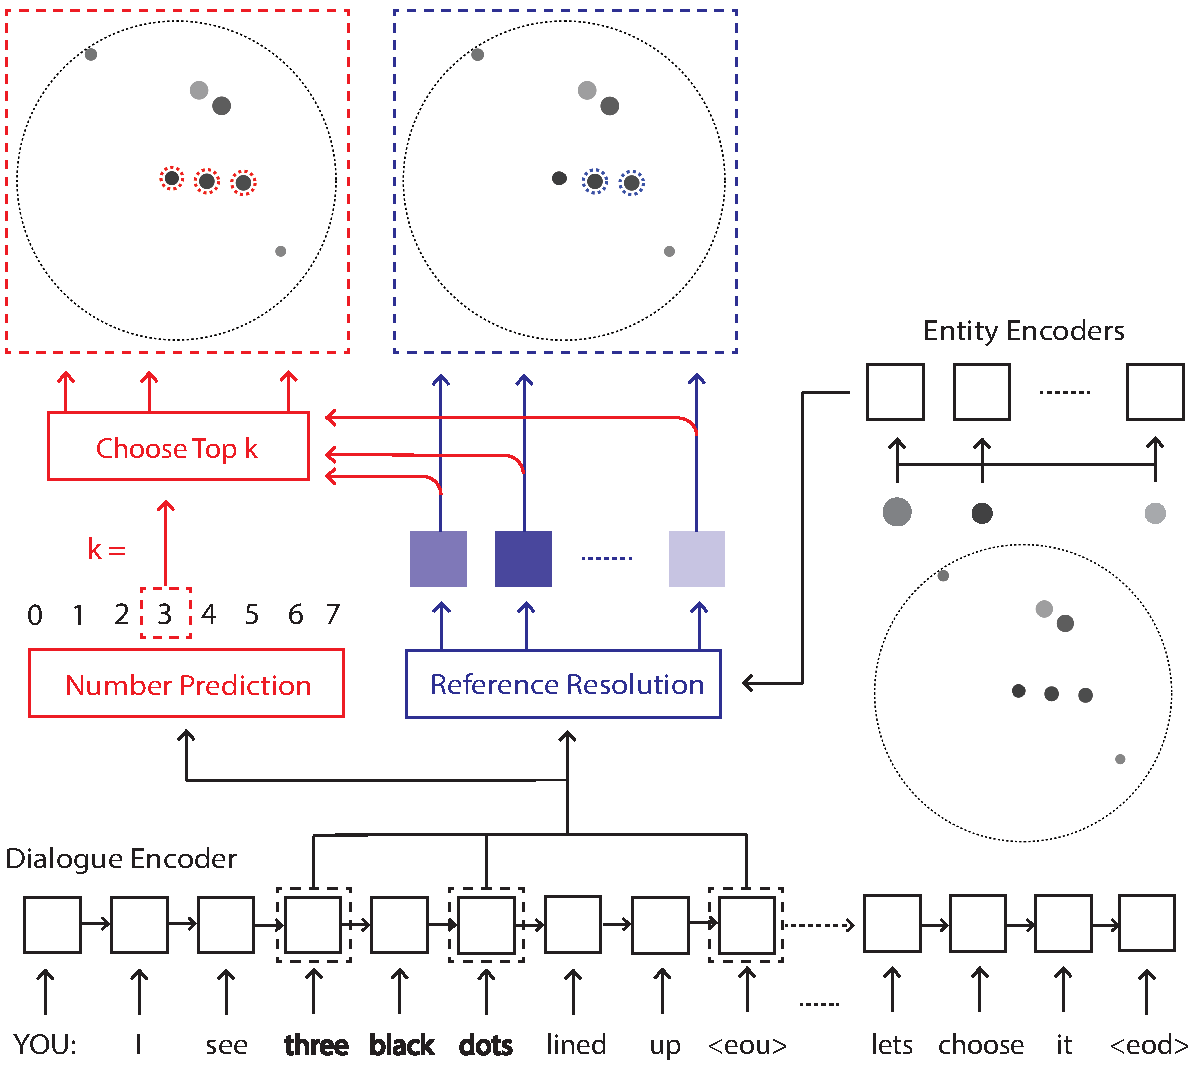
\includegraphics[width=0.7\columnwidth]{model_architecture.pdf}
\caption{Our model architecture. REF prediction flow is shown in blue and our NUMREF prediction flow in red.}
\label{05_fig:model_architecture}
\end{figure}

As a baseline, we use the \textit{REF} model from Chapter \ref{04_chp:interpretation}. As shown in Figure \ref{05_fig:model_architecture}, this model has two encoders: a \textit{dialogue encoder} based on a simple GRU \citep{cho2014properties} and a shared \textit{entity encoder} which outputs entity-level representation of the observation based on MLP and relational network \citep{santoro2017simple}. To predict the referents, REF takes the GRU's start position of the markable, end position of the markable and end position of the utterance to compute entity-level scores and judge whether each entity is a referent based on logistic regression.

However, since the predictions are made independently for each entity, this model often predicts the wrong number of referents, leading to low performance in terms of exact match rate. To address this issue, we trained a separate module to track the \textit{number} of referents in each markable. We formulate this as a simple classification task (between 0, 1, ..., 7) which can be predicted reliably with an average accuracy of $92$\%. Based on this module's prediction $k$, we simply take the top $k$ entities with the highest scores as the referents. We refer to this numerically constrained model as NUMREF.

Furthermore, we conduct feature level ablations to study the importance of each feature: for instance, we remove the xy-values from the structured input to ablate the \textit{location} feature.

\subsection{Results}
\label{05_subsec:reference_resolution_results}

\begin{table}[ht]
\centering \small
\setlength{\tabcolsep}{9pt}
\begin{tabular}{lcc}
\toprule
 & Entity-Level & Markable-Level \\
 & Accuracy (\%) & Exact Match (\%) \\
\midrule
REF & 85.71$\pm$0.23 & 33.15{\scriptsize $\pm$1.00} \\
\phantom{NN}$-$ location & 84.28{\scriptsize $\pm$0.27} & 30.53{\scriptsize $\pm$0.84} \\
\phantom{NN}$-$ color & 83.08{\scriptsize $\pm$0.32} & 17.09{\scriptsize $\pm$1.04} \\
\phantom{NN}$-$ size & 83.50{\scriptsize $\pm$0.22} & 19.41{\scriptsize $\pm$0.98} \\
\midrule
NUMREF & \textbf{86.03{\scriptsize $\pm$0.33}} & \textbf{54.94{\scriptsize $\pm$0.76}} \\
\phantom{NN}$-$ location & 83.35{\scriptsize $\pm$0.26} & 49.77{\scriptsize $\pm$0.64} \\
\phantom{NN}$-$ color & 81.19{\scriptsize $\pm$0.41} & 39.74{\scriptsize $\pm$1.31} \\
\phantom{NN}$-$ size & 82.39{\scriptsize $\pm$0.20} & 43.40{\scriptsize $\pm$0.67} \\
\midrule
Human & 96.26 & 86.90 \\
\bottomrule
\end{tabular}
\caption{
Results for the reference resolution task.
}
\label{05_tab:experiment_results}
\end{table}

We report the mean and standard deviation of the entity-level accuracy and markable-level exact match rate in Table \ref{05_tab:experiment_results}. Compared to REF, our NUMREF model slightly improves the entity-level accuracy and significantly outperforms it in terms of exact match rate, which validates our motivation. From the ablation studies, we can see that all features contribute to the overall performance, but color and size seem to have the largest impact. 

However, it remains difficult to see how and where these models struggle based on mere accuracy. For further investigation, we need more sophisticated \textit{behavioral testing} (black-box testing) to verify whether each model has the capability of recognizing certain concepts or linguistic structures \citep{ribeiro-etal-2020-beyond}.

\section{Model Analysis}
\label{05_sec:model_analysis}

To study the current model's strengths and weaknesses in detail, we investigate whether their predictions are \textit{consistent} with the central spatial expressions.

\subsection{Spatial Attributes}
\label{05_subsec:spatial_attributes}

\begin{figure}[ht]
\centering
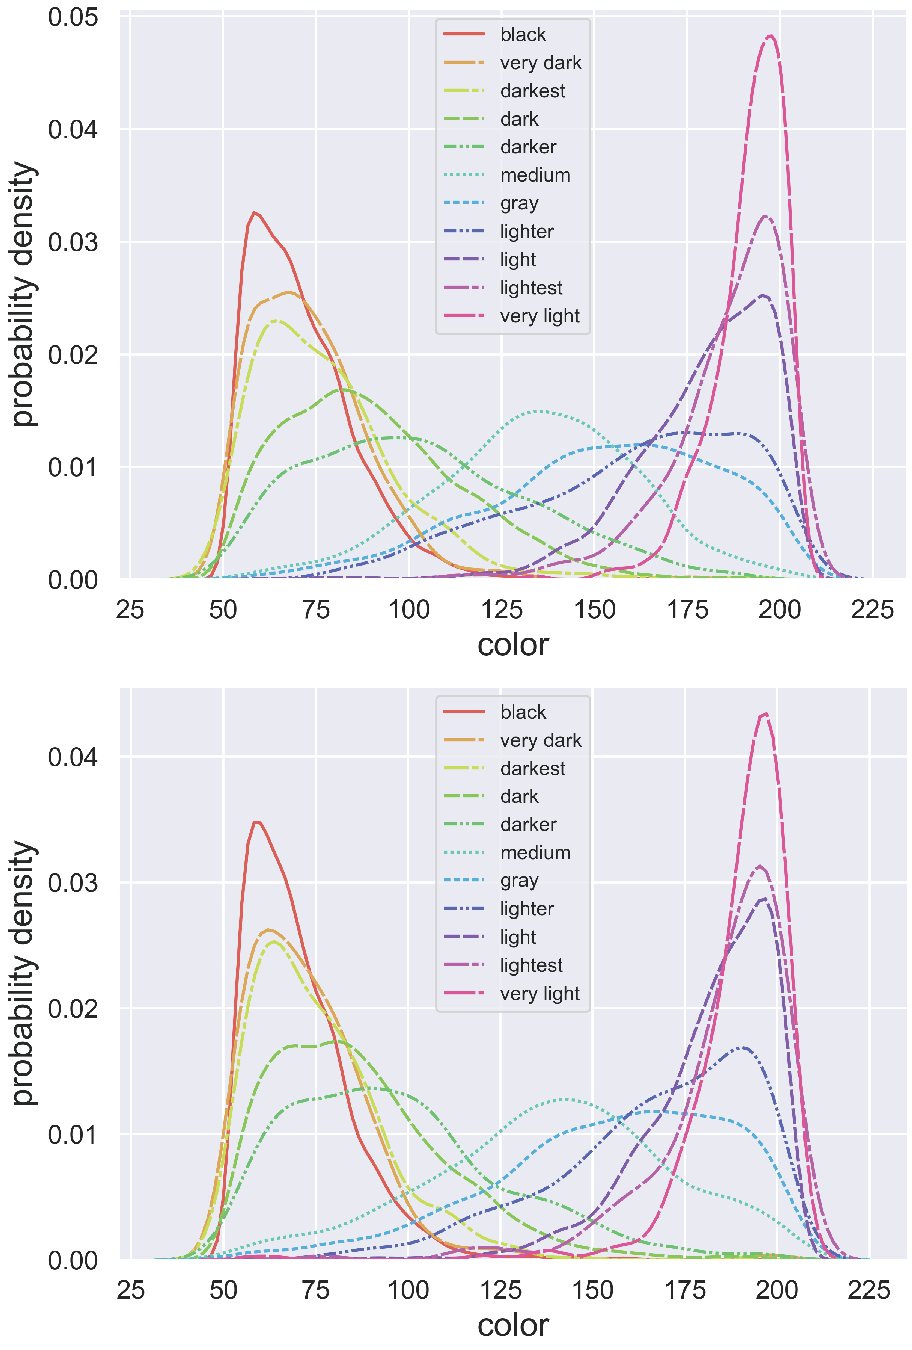
\includegraphics[width=0.6\columnwidth]{referent_color.pdf}
\caption{Referent color distributions. Top is human, bottom is NUMREF (smaller is darker in color axis).}
\label{05_fig:referent_color}
\end{figure}

First, we analyze whether the model predictions are consistent with the entity-level spatial attributes. Since most of them were confirmed to appear inside the markables (Section \ref{05_sec:annotation_results}), we automatically detect the expressions of \textit{color} in the markables, plot the distributions of the actual referent color, and compare the results between gold human annotation and model predictions (Figure \ref{05_fig:referent_color}).

From the figure, we can verify that the two distributions look almost identical for the common color expressions, and our NUMREF model seems to capture important characteristics of pragmatic expressions (same expression being used for wide range of colors) and modifications such as neutrality (\textit{medium}) and extremity (\textit{very dark}, \textit{very light}).\footnote{Spatial attributes with diminishers (such as \textit{slightly dark}) were relatively rare and omitted in the figure.} Note that we observed very similar results with the \textit{size} distributions as well.

Based on these results, we argue that the current model can capture entity-level attributes very well, including basic modification.

\subsection{Spatial Relations}
\label{05_subsec:spatial_relations}

\begin{table*}[th]
\centering \scalebox{0.77}{
\small
\def\arraystretch{1.0}
\newcommand{\intermidrule}{\cmidrule{2-13}}  
\setlength{\tabcolsep}{4pt}
\setlength{\aboverulesep}{0pt}
\setlength{\belowrulesep}{0pt}
\setlength{\extrarowheight}{.75ex}
\begin{tabular}{lcc|cacacacaca}
\toprule
\multicolumn{3}{c}{Models} & \multicolumn{2}{c}{REF} & \multicolumn{2}{c}{REF-abl} & \multicolumn{2}{c}{NUMREF} & \multicolumn{2}{c}{NUMREF-abl} & \multicolumn{2}{c}{Human} \\
\midrule
Category & Relation & \# Cases  & satisfy & \phantom{.}valid\phantom{.} & satisfy & \phantom{.}valid\phantom{.} & satisfy & \phantom{.}valid\phantom{.} & satisfy & \phantom{.}valid\phantom{.} & satisfy & \phantom{.}valid\phantom{.} \\
\midrule
\multirow{8}{*}{Direction}\phantom{..} & \textit{left} & 412 & 23.5 & 32.3 & 21.1 & 28.9 & \textbf{67.0} & \textbf{99.5} & 62.4 & \textbf{99.5} & 95.9 & 97.6 \\
 & \textit{right} & 468 & 28.0 & 35.5 & 24.6 & 30.8 & 67.3 & \textbf{98.7} & \textbf{68.2} & \textbf{98.7} & 95.3 & 96.4 \\
 & \textit{above} & 514 & 28.6 & 37.4 & 24.7 & 33.1 & 65.2 & 99.2 & \textbf{66.5} & \textbf{99.4} & 96.7 & 98.6 \\
 & \textit{below} & 444 & 25.2 & 34.5 & 21.6 & 27.9 & \textbf{66.0} & \textbf{99.1} & 62.2 & \textbf{99.1} & 96.4 & 96.8 \\
 & \textit{horizontal} & 37 & 54.1 & 70.3 & 27.0 & 59.5 & \textbf{59.5} & \textbf{100.0} & 51.4 & 97.3 & 91.9 & 100.0 \\
 & \textit{vertical} & 46 & 37.0 & 73.9 & 23.9 & 54.3 & 43.5 & \textbf{95.7} & \textbf{45.7} & \textbf{95.7} & 82.6 & 100.0 \\
 & \textit{diagonal} & 50 & 48.0 & 74.0 & 30.0 & 50.0 & \textbf{60.0} & \textbf{98.0} & \textbf{60.0} & \textbf{98.0} & 90.0 & 100.0 \\
\intermidrule
 & All & 1,971 & 27.8 & 37.6 & 23.4 & 31.9 & \textbf{65.5} & \textbf{99.0} & 64.1 & \textbf{99.0} & 95.5 & 97.6 \\
\midrule
\multirow{4}{*}{Proximity} & \textit{near} & 271 & 49.4 & 61.3 & 29.9 & 49.1 & \textbf{77.1} & 94.5 & 56.1 & \textbf{95.2} & 95.2 & 96.7 \\
 & \textit{far} & 27 & 29.6 & 40.7 & 33.3 & 40.7 & 77.8 & \textbf{100.0} & \textbf{92.6} & \textbf{100.0} & 96.3 & 96.3 \\
 & \textit{alone} & 111 & 36.9 & 44.1 & 45.0 & 54.1 & \textbf{68.5} & \textbf{94.6} & 67.6 &\textbf{94.6} & 91.9 & 94.6 \\
\intermidrule
 & All & 409 & 44.7 & 55.3 & 34.2 & 49.9 & \textbf{74.8} & 94.9 & 61.6 & \textbf{95.4} & 94.4 & 96.1 \\
\midrule
\multirow{3}{*}{Region} & \textit{interior} & 135 & 38.5 & 52.6 & 27.4 & 39.3 & \textbf{62.2} & 93.3 & 58.5 & \textbf{94.1} & 96.3 & 100.0 \\
 & \textit{exterior} & 62 & 40.3 & 48.4 & 40.3 & 53.2 & 80.6 & \textbf{98.4} & \textbf{87.1} & \textbf{98.4} & 98.4 & 98.4 \\
\intermidrule
 & All & 197 & 39.1 & 51.3 & 31.5 & 43.7 & \textbf{68.0} & 94.9 & 67.5 & \textbf{95.4} & 97.0 & 99.5 \\
\midrule
\multirow{7}{*}{Color} & \textit{lighter} & 147 & 23.1 & 25.9 & 6.8 & 8.2 & \textbf{84.4} & \textbf{100.0} & 57.1 & 99.3 & 97.3 & 98.0 \\
 & \textit{lightest} & 42 & 45.2 & 66.7 & 14.3 & 33.3 & \textbf{61.9} & \textbf{100.0} & 31.0 & \textbf{100.0} & 83.3 & 100.0 \\
 & \textit{darker} & 171 & 24.0 & 26.3 & 7.0 & 10.5 & \textbf{83.0} & \textbf{99.4} & 53.2 & \textbf{99.4} & 95.9 & 98.8 \\
 & \textit{darkest} & 48 & 56.2 & 64.6 & 14.6 & 33.3 & \textbf{66.7} & \textbf{100.0} & 35.4 & \textbf{100.0} & 89.6 & 97.9 \\
 & \textit{same} & 50 & 12.0 & 30.0 & 8.0 & 30.0 & \textbf{40.0} & \textbf{88.0} & 32.0 & 86.0 & 92.0 & 96.0 \\
 & \textit{different} & 14 & 64.3 & 71.4 & 71.4 & 71.4 & 64.3 & \textbf{100.0} & \textbf{78.6} & 92.9 & 92.9 & 100.0 \\
\intermidrule
 & All & 472 & 28.8 & 35.4 & 10.4 & 18.0 & \textbf{74.8} & \textbf{98.5} & 49.2 & 97.9 & 94.1 & 98.3 \\
\midrule
\multirow{7}{*}{Size} & \textit{smaller} & 213 & 27.7 & 31.5 & 7.5 & 9.9 & \textbf{80.8} & \textbf{100.0} & 59.6 & \textbf{100.0} & 98.6 & 99.5 \\
 & \textit{smallest} & 52 & 71.2 & 73.1 & 21.2 & 34.6 & \textbf{86.5} & \textbf{98.1} & 48.1 & \textbf{98.1} & 92.3 & 98.1 \\
 & \textit{larger} & 238 & 23.1 & 28.6 & 9.7 & 16.0 & \textbf{73.5} & \textbf{99.6} & 48.7 & \textbf{99.6} & 98.3 & 98.3 \\
 & \textit{largest} & 61 & 52.5 & 60.7 & 11.5 & 24.6 & \textbf{73.8} & \textbf{100.0} & 39.3 & \textbf{100.0} & 96.7 & 100.0 \\
 & \textit{same} & 103 & 34.0 & 42.7 & 18.4 & 27.2 & \textbf{80.6} & 88.3 & 65.0 & \textbf{91.3} & 98.1 & 100.0 \\
 & \textit{different} & 12 & 75.0 & 75.0 & 66.7 & 66.7 & \textbf{91.7} & \textbf{91.7} & 83.3 & 83.3 & 91.7 & 91.7 \\
\intermidrule
 & All & 679 & 33.4 & 38.7 & 12.4 & 18.9 & \textbf{78.2} & 97.8 & 54.3 & \textbf{98.1} & 97.6 & 99.0 \\
\bottomrule
\end{tabular}
}
\caption{
Canonical relation test results. We compute the \textit{satisfy} and \textit{valid} rate of the predictions for each canonical relation. Best scores of the models are in bold (-abl shows the corresponding feature ablated results).
}
\label{05_tab:satisfication_result}
\end{table*}

Next, we investigate whether the model predictions are consistent with the central spatial relations. Based on our annotation (Section \ref{05_sec:annotation_procedure}), we conduct simple tests to check whether the predicted referents satisfy each canonical relation. To be specific, our tests check for two conditions: whether the predictions are \textit{valid} (satisfy the minimal requirements, e.g. at least 2 referents predicted for \textit{near} relation), and if they are valid, whether the predictions actually \textit{satisfy} the canonical relation (e.g. referents are closer than a certain threshold).

Algorithm \ref{alg:left} shows our test for the canonical \textit{left} relation. Note that if no objects were annotated, we simply test whether the subject referents are on the left side of the player's view ($ mean(\mathcal{S}.x) < 0 $).

\begin{algorithm}[h]
\small
\DontPrintSemicolon
\SetAlgoNoEnd

\KwIn{subject referents $\mathcal{S}$, object referents $\mathcal{O}$, boolean $no\_object$}
\KwOut{boolean $satisfy$, boolean $valid$}
\If{$no\_object$}{
	$valid \leftarrow |\mathcal{S}| \! > \! 0$\\
	$satisfy \leftarrow valid \, \wedge \, mean(\mathcal{S}.x) \! < \! 0$
}\Else{
	$valid \leftarrow |\mathcal{S}| \! > \! 0 \, \wedge \, |\mathcal{O}| \! > \! 0$\\
	$satisfy \leftarrow valid \, \wedge \, mean(\mathcal{S}.x) \! < \! mean(\mathcal{O}.x)$
}
\Return $satisfy$, $valid$
\caption{Test for \textit{left} relation}
\label{alg:left}
\end{algorithm}

The results of our tests are summarized in Table \ref{05_tab:satisfication_result}. We also compare with the feature ablated models to estimate the test cases which can be satisfied \textit{without} using the corresponding features, i.e. location for \textit{direction}/\textit{proximity}/\textit{region} categories, color for \textit{color comparison}, and size for \textit{size comparison}.

First, we can verify that human annotation passes most of our tests, which is an important evidence of the reliability of our annotations and behavioral tests. We also confirmed that REF models often make \textit{invalid} predictions with overall poor performance, which is consistent with our expectation.

In \textit{direction}, \textit{proximity} and \textit{region} categories, we found that NUMREF model performs on par or only marginally better than its ablated version (and even underperforms it for simple relations like \textit{right} and \textit{above}): these results indicate that current model is still incapable of leveraging locational features to make more consistent predictions.\footnote{For relations like \textit{far} and \textit{different color}, ablated model may be better simply because referents tend to be more distant/dissimilar when predictions are closer to random.}

In \textit{color/size comparison}, NUMREF performs reasonably well, outperforming all other models: this indicates that the model can not only capture but also \textit{compare} entity-level attributes to a certain extent. However, there is still room left for improvement in almost all relations. It is also worth noting that \textit{size comparison} may be easier, as the range of size is limited (only \textit{6} compared to \textit{150} for color).

Overall, we conclude that current models still struggle in capturing most of the inter-entity relations, especially those related to placements.

\subsection{Further Analyses}
\label{05_subsec:further_analyses}

\begin{table}[h!]
\centering \small
\begin{tabular}{lccc}
\toprule
Linguistic Factors & \# Cases & NUMREF & Human  \\
 \midrule
Strong modification & 149 & 76.51 & 95.97 \\
Neutral & 3,094 & 70.46 & 95.77 \\
Weak modification & 490 & 66.12 & 95.10 \\
\midrule
Inter-utterance subject & 14 & 57.14 & 92.86 \\
Inter-utterance object & 265 & 72.08 & 94.72 \\
No object & 1,127 & 74.45 & 92.99 \\
Ignorable object & 1,805 & 69.64 & 97.23 \\
Unignorable object & 796 & 65.33 & 96.11 \\
\midrule
All & 3,728 & 70.17 & 95.71 \\
\bottomrule
\end{tabular}
\caption{
Satisfy rates classified by linguistic factors.
}
\label{further comparison}
\end{table}

Finally, we conduct further analyses to study other linguistic factors that affect model performance. Table \ref{further comparison} shows the results of our relation tests classified by notable linguistic structures.

In terms of modification, we can confirm that human performance is consistently high, while the model performs best for strong modification (modified by \textit{boosters} or \textit{maximizers}), decently for neutrals (\textit{moderators} or no modification), and worst on weak modification (\textit{diminishers} or \textit{approximators}). This indicates that large, conspicuous features are easier for the model to capture compared to small or more ambiguous features.

In terms of subject/object properties, human performance is also consistently high. In contrast, model performance is significantly worse for subject ellipsis (\textit{inter-utterance subject}), while remaining high for object ellipsis and \textit{no object} cases.

We also hypothesize that a large portion of the relations can actually be satisfied \textit{without} considering the objects, e.g. by simply predicting very dark dots as the subjects when the relation is \textit{darker} or \textit{darkest}. To distinguish such easy cases, we consider a relation as \textit{ignorable object} if the relation can be satisfied even if we ignore the objects (i.e. remove all object relations) based on gold referents. Our result verifies that there are indeed many cases of \textit{ignorable object}, and they seem slightly easier for the model to satisfy.

\begin{table}[h!]
\centering \small
\def\arraystretch{1.0}
\newcommand{\intermidrule}{\cmidrule{2-13}}  
\setlength{\tabcolsep}{4pt}
\setlength{\aboverulesep}{0pt}
\setlength{\belowrulesep}{0pt}
\setlength{\extrarowheight}{.75ex}
\begin{tabular}{lccaca}
\toprule
\multicolumn{2}{c}{Models} & \multicolumn{2}{c}{NUMREF} & \multicolumn{2}{c}{Human} \\
\midrule
value & mod-type & diff. & \# valid & diff. & \# valid \\
\midrule
\multirow{3}{*}{xy-value} & strong & 86.06 & 39 & 89.15 & 37 \\
& neutral & 80.92 & 1,586 & 73.52 & 1,558\\
& weak & 80.35 & 200 & 53.53 & 198 \\
\midrule
\multirow{3}{*}{color} & strong & 66.23 & 15 & 91.80 & 15 \\
& neutral & 56.98 & 234 & 60.14 & 232\\
& weak & 37.73 & 68 & 28.55 & 66 \\
\midrule
\multirow{3}{*}{size} & strong & 3.60 & 8 & 4.29 & 8 \\
& neutral & 2.67 & 337 & 2.70 & 320\\
& weak & 1.95 & 105 & 1.58 & 104 \\
\bottomrule
\end{tabular}
\caption{
Absolute differences of feature values in comparative relations (number of valid predictions shown in shade).
}
\label{05_tab:difference_comparison}
\end{table}

In Table \ref{05_tab:difference_comparison}, we study the effect of modification based on the  \textit{absolute difference} between subject and object features in comparative relations.\footnote{\textit{Left/right} for x-value, \textit{above/below} for y-value, \textit{lighter/darker} for color and \textit{smaller/larger} for size.}

In human annotation, the absolute difference naturally increases as the modification gets stronger. While model predictions also show this tendency, their results seem less sensitive to modification (particularly for locational features, i.e. xy-value) and may not be reflecting their full effect.

\section{Related Work}
\label{05_sec:related_work}

Linguistic structure plays a critical role in dialogue research. From theoretical aspects, various dialogue structures have been studied, including discourse structure \citep{stent-2000-rhetorical,asher2003logics}, speech act \citep{austin1962things,searle1969speech} and common grounding \citep{clark1996using,lascarides2009agreement}. In dialogue system engineering, various linguistic structures have been considered and applied, including syntactic dependency \citep{davidson-etal-2019-dependency}, predicate-argument structure \citep{yoshino2011spoken}, ellipsis \citep{quan-etal-2019-gecor,hansen2020you}, intent recognition \citep{silva2011symbolic,shi-etal-2016-deep}, semantic representation/parsing \citep{mesnil2013investigation,gupta-etal-2018-semantic} and frame-based dialogue state tracking \citep{williams2016dialog,elasri2017frames}. However, most prior work focus on dialogues where information is not grounded in external, perceptual modality such as vision. In this work, we propose an effective method of analyzing linguistic structures in visually grounded dialogues.

Recent years have witnessed an increasing attention in visually grounded dialogues \citep{zarriess-etal-2016-pentoref,de2018talk,alamri2019audio,narayan-chen-etal-2019-collaborative}. Despite the impressive progress on benchmark scores and model architectures \citep{Das_2017_ICCV,Wu_2018_CVPR,Kottur_2018_ECCV,gan-etal-2019-multi,shukla-etal-2019-ask,niu2019recursive,zheng2019reasoning,kang-etal-2019-dual,visdial_bert,pang2020visual}, there have also been critical problems pointed out in terms of dataset biases \citep{goyal2017making,visdial_eval,massiceti2018visual,chen-etal-2018-attacking,kottur-etal-2019-clevr,kim2020modality,agarwal-etal-2020-history} which obscure such contributions. For instance, \citet{cirik-etal-2018-visual} points out that existing dataset of reference resolution may be largely solvable \textit{without} recognizing the full referring expressions (e.g. based on object categories only). To circumvent these issues, we focused on our OneCommon Corpus where the visual contents are simple (exploitable categories are removed) and well-balanced (by sampling from uniform distributions) to minimize dataset biases.

Although various probing methods have been proposed for models and datasets in NLP \citep{belinkov-glass-2019-analysis,geva-etal-2019-modeling,kaushik2019learning,gardner2020evaluating,ribeiro-etal-2020-beyond}, fine-grained analyses of visually grounded dialogues have been relatively limited. Instead, \citet{kottur-etal-2019-clevr} proposed a diagnostic dataset to investigate model's language understanding: however, their dialogues are generated artificially and may not reflect the true nature of visual dialogues. \citet{shekhar-etal-2019-beyond} also acknowledges the importance of linguistic analysis but only dealt with coarse-level features that can be computed automatically (such as dialogue topic and diversity). Most similar and related to our research are \citet{yu-etal-2019-see} and \citet{udagawa2020annotated}, where they conducted additional annotation of reference resolution in visual dialogues: however, they still do not capture more sophisticated linguistic structures such as predicate-argument structure, modification and ellipsis.

Finally, spatial language and cognition have a long history of research \citep{talmy1983language,herskovits1987language}. In computational linguistics, \citet{kordjamshidi-etal-2010-spatial} and \citet{pustejovsky2015semeval} developed the task of spatial role labeling to capture spatial information in text: however, they do not fully address the problem of annotation reliability nor grounding in external visual modality. In computer vision, the VisualGenome dataset \citep{krishna2017visual} provides rich annotation of spatial scene graphs constructed from raw images, but not from raw dialogues. \citet{ramisa-etal-2015-combining} and \citet{platonov2018computational} also worked on modelling spatial prepositions in single sentences. To the best of our knowledge, our work is the first to apply, model and analyze spatial expressions in visually grounded dialogues at full scale.

\section{Discussion and Conclusion}
\label{05_sec:conclusion}

In this study, we focused on the (annotated) OneCommon Corpus as a suitable testbed for fine-grained language understanding in visually grounded dialogues. To analyze its linguistic structures, we proposed a novel framework of annotating spatial expressions in visual dialogues. We showed that our annotation can be conducted reliably and efficiently by leveraging referring expressions prevalent in visual dialogues, while capturing important linguistic structures such as predicate-argument structure, modification and ellipsis. Although our current analysis is limited to this domain, we expect that upon appropriate definition of spatial expressions, argument roles and canonicalization, the general approach can be applied to a wider variety of domains: adapting and validating our approach in different domains (especially with more realistic visual contexts) are left as future work.

Secondly, we proposed a simple idea of incorporating \textit{numerical constraints} to improve exophoric reference resolution. We expect that a similar approach of identifying and incorporating semantic constraints (e.g. coreferences and spatial constraints) is a promising direction to improve the model's performance even further.

Finally, we demonstrated the advantages of our annotation for investigating the model's understanding of visually grounded dialogues. Our tests are completely agnostic to the models and only require referent predictions made by each model. By designing simple tests like ours (Sections \ref{05_subsec:spatial_attributes} and \ref{05_subsec:spatial_relations}), we can diagnose the model's performance at the granularity of canonical attributes/relations under consideration: such analyses are easy to extend (by adding more tests) and critical for verifying what capabilities current models have (or do not have). Based on further analyses (Section \ref{05_subsec:further_analyses}), we also revealed various linguistic structures that affect model performance: we expect that capturing and studying such effects will be essential for advanced model probing in visual dialogue research.

Overall, we expect our framework and resource to be fundamental for conducting sophisticated linguistic analyses of visually grounded dialogues, involving advanced common grounding and symbol grounding.


\graphicspath{{06_task_generalization/figures/}} % Location of the graphics files

\chapter{Task Generalization under Dynamic Context}
\label{06_chp:task_generalization}

Common grounding is the process of creating and maintaining mutual understandings, which is a critical aspect of sophisticated human communication. While various task settings have been proposed in existing literature, they mostly focus on creating common ground under static context and ignore the aspect of \textit{maintaining} them overtime under \textit{dynamic} context. In this chapter, we propose a novel task setting to study the ability of both creating and maintaining common ground in dynamic environments. Based on our minimal task formulation, we collected a large-scale dataset of 5,617 dialogues to enable fine-grained evaluation and analysis of various dialogue systems. Through our dataset analyses, we highlight novel challenges introduced in our setting, such as the usage of complex \textit{spatio-temporal expressions} to create and maintain common ground. Finally, we conduct extensive experiments to assess the capabilities of our baseline dialogue system and discuss future prospects of our research.

\section{Introduction}
\label{06_sec:introduction}

Common grounding is the process of creating, repairing and updating mutual understandings (i.e. \textit{common ground}), which is a critical aspect of sophisticated human communication \citep{clark1996using}. Humans can \textit{create} substantial common ground by expressing various information in natural language, which can be clarified or \textit{repaired} to resolve misunderstandings at essential levels of detail. Furthermore, as the situation changes and relevant information gets outdated, humans can \textit{update} their common ground accordingly by discarding old information and acquiring new ones. Such ability plays a vital role in sustaining collaborative relationships and adapting to emerging problems in nonstationary, real-world environments.

However, despite the wide variety of tasks proposed in existing literature \citep{fang2015embodied,zarriess-etal-2016-pentoref,de2017guesswhat,udagawa2019natural,haber-etal-2019-photobook}, they mostly focus on creating common ground under \textit{static} (time-invariant) context and ignore their \textit{dynamic} aspects. While some recent dialogue tasks deal with dynamic information, they often lack suitable evaluation metrics \citep{pasunuru-bansal-2018-game}, \textit{context updates} in the course of the dialogue \citep{alamri2019audio} or diverse dynamics of the environment itself \citep{de2018talk,suhr-etal-2019-executing,narayan-chen-etal-2019-collaborative,thomason:corl19,moon-etal-2020-situated}. Therefore, it remains unclear how well existing dialogue systems can adapt to the diversely changing situations through advanced common grounding.

To address this problem, we propose a novel dialogue task based on three design choices (Section \ref{06_sec:task_formulation}):

First, we formulate a novel \textit{sequential collaborative reference task} as a temporal generalization of the collaborative reference task proposed in Chapter \ref{03_chp:task_formulation}. In our formulation, the goal of the agents is generalized to track and select the common entity \textit{at multiple timesteps}, while the agents' observations change dynamically between each timestep. This setting requires both \textit{creation} and \textit{maintenance} of common ground, whilst enabling clear evaluation based on the length of successful timesteps.

Secondly, we focus on synthesizing the \textit{entity movements}, as popularized in the recent video understanding benchmarks \citep{girdhar2020cater,yi2020clevrer,bakhtin2019phyre}. By leveraging such synthetic dynamics, we can minimize undesirable biases, maximize diversity and enable fully controlled evaluation and analysis.

Finally, we build upon our OneCommon Corpus to introduce natural difficulty of common grounding with minimal task complexity. To be specific, we represent entity attributes and their temporal dynamics based on \textit{continuous} real values to introduce high ambiguity and uncertainty. In addition, we consider a \textit{partially-observable} setting where each agent only has a partial view of the environment, which introduces various misunderstandings and partial understandings that need to be resolved.

Based on this task design, we collected a large-scale dataset of 5,617 dialogues (including over 65K utterances) through careful crowdsourcing on Amazon Mechanical Turk (Section \ref{06_sec:dataset_collection}).

\begin{figure*}[tb!]
\centering
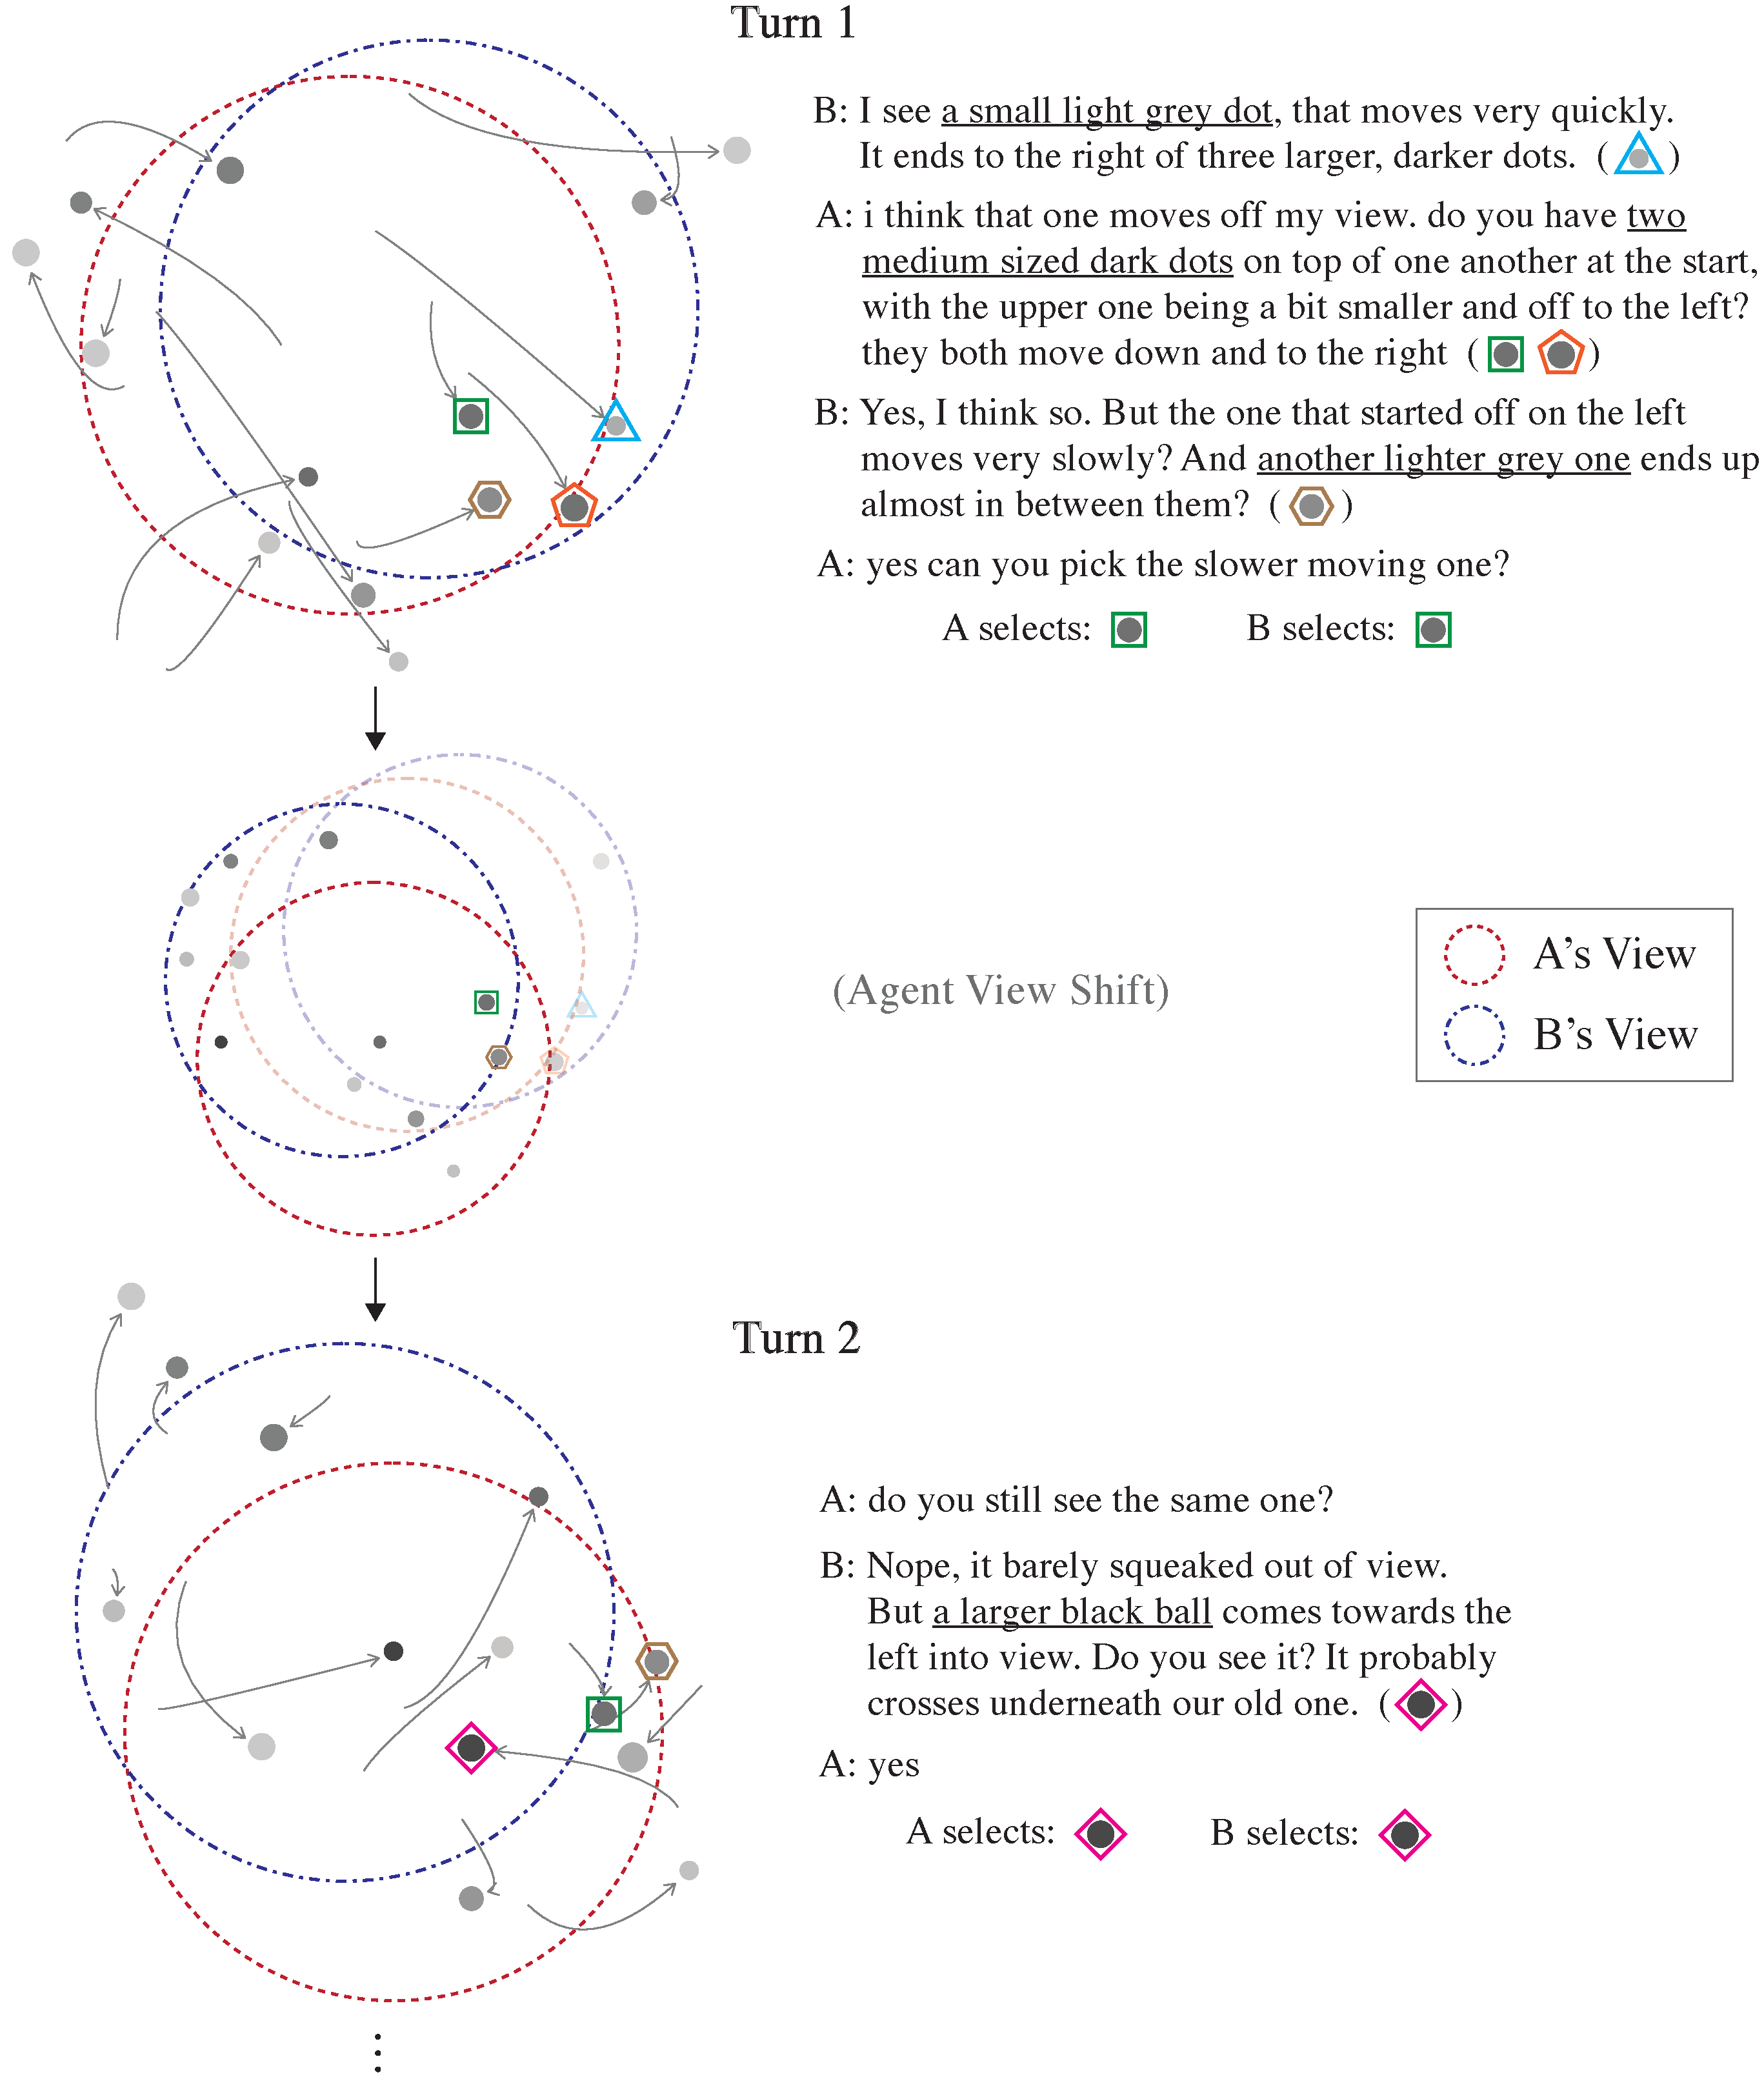
\includegraphics[width=\textwidth]{first_example.pdf}
\caption{Example dialogue of our sequential collaborative reference task. Each agent has a partial view of a 2-D plane with synthetic entities (grayscale dots of various sizes). \textit{During} each turn, the entities move randomly on the 2-D plane. \textit{At the end} of each turn, the agents communicate with each other to find and select one of the same, common entities. \textit{After} each turn (if the selections match), both agents' views shift randomly and the next turn begins.
}
\label{06_fig:first_example}
\end{figure*}

We show an exemplary dialogue of our task in Figure \ref{06_fig:first_example}. Since the environment is dynamic, humans rely on various \textit{spatio-temporal expressions} to express entity states at different timesteps (``\underline{started off} on the left'', ``\underline{ends} to the right'') or how they changed dynamically (``moves very quickly'', ``come towards the left'') to create common ground. Furthermore, in later turns, humans often leverage their \textit{previous common ground} (``still see the same one?'', ``crosses underneath our old one'') to update their common ground more reliably and efficiently. We conduct detailed analyses of the dataset to study such strategies in Section \ref{06_sec:dataset_analysis}.

In our experiments (Section \ref{06_sec:experiments}), we train a neural-based dialogue system based on \citet{udagawa2020annotated}. Through our extensive evaluation and analysis, we assess the current model's strengths as well as important limitations and demonstrate huge room left for further improvement.

Overall, the contributions of this chapter are as follows:

\begin{itemize}
    \item We proposed a novel dialogue task to study common grounding in dynamic environments.
    \item We collected a large-scale dataset of 5,617 dialogues to develop and test various data-driven models.
    \item Our detailed dataset analyses highlight novel challenges introduced in our setting.
    \item We conduct extensive evaluation and analysis of a simple yet strong baseline dialogue system.
\end{itemize}

\section{Task Formulation}
\label{06_sec:task_formulation}

In this section, we review the collaborative reference task from OneCommon Corpus (OCC in short) and formulate our \textit{sequential} counterpart as its temporal generalization.


\subsection{Collaborative Reference Task}
\label{06_subsec:collaborative_reference_task}

Based on \citet{udagawa2019natural}, a \textit{collaborative reference task} is a multi-agent cooperative game with entities $E = \{e_1, e_2, ... , e_m\}$ and agents $A = \{a_1, a_2, ... , a_n\}$. Each agent $a_j \in A$ has an observation of entities $obs_j(E)$ and can exchange information with other agents in natural language. At the end of the game, each agent selects one of the observable entities, and the game is \emph{successful} if and only if all the agents selected the same entity. This can be considered as a general framework for evaluating accurate \textit{mutual recognition} of a common entity, which is often a critical step in general common grounding.

One main feature of OCC is that they represented all entity attributes (color, size and location on a 2-D plane) based on \textit{continuous} real values. Unlike discrete/categorical attributes, this introduces high ambiguity and uncertainty to be expressed in symbolic natural language. In addition, they introduced \textit{partial-observability} where each agent only has a partial view of the 2-D plane, which requires collaborative resolution of various misunderstandings.

However, this current task formulation assumes each observation to be \textit{static} and can only evaluate the ability of \textit{creating} common ground.

\subsection{Sequential Collaborative Reference Task}
\label{06_subsec:sequential_collaborative_reference_task}

To address this limitation, we generalize each observation to be \textit{dynamic} and collaborative reference to be \textit{sequential}. Specifically, each agent $a_j \in A$ now receives observation $obs_j(E, t)$ at each timestep $t \in [t_0, \infty)$, and the agents' goal is to communicate in natural language to select the same entity at multiple timesteps $t_1, t_2, ... \in (t_0, \infty)$.\footnote{We assume $t_{k -1} < t_k $ for all $k \in \mathbb{N}$.} At each selection timestep $t_k$ ($k \in \mathbb{N}$), $a_j$ must select one entity observable at $t_k$ but has all previous observations up to $t_k$, $\{obs_j(E, t) | t \in [t_0, t_k] \}$. The game ends when the selections no longer match at timestep $t_{k^\prime}$ ($k^\prime \in \mathbb{N}$): therefore, the success at $t_1$ measures the ability of \textit{creating} common ground, and the length of successful timesteps (LST) $k^\prime-1$ measures the ability of \textit{maintaining} them. This is a general framework for evaluating both creation and maintenance of mutual entity recognition in dynamic environments.

Based on this task formulation, we propose a minimal task setting extending OCC and incorporate dynamic change of the entity \textit{locations}.

We refer to each time range $[t_{k-1}, t_k]$ as \textit{turn} $k$. During each turn, we change the location of each entity $e_i \in E$ based on a simple parameterized movement, where the \textit{trajectory} is determined by a quadratic B\'{e}zier curve \citep{bezier1974mathematical}.\footnote{Its \textit{speed} is proportional to the length of the trajectory.} See Figure \ref{06_fig:entity_movement} for an illustration, where $r_{1}$, $r_{2}$ are parameters of \textit{distance} and $\theta_{k-1}$, $\Delta \theta$ represent \textit{angles}. We sample $r_{1}$, $r_{2}$, $\Delta \theta$ from fixed uniform distributions each turn and update $\theta_{k}$ as $\theta_{k} \leftarrow \theta_{k-1} + \Delta \theta$ ($\theta_{0}$ is initialized randomly). This way, we can generate diverse, unbiased, coherent and fully controllable dynamics of the environment.

\begin{figure}[th]
\centering
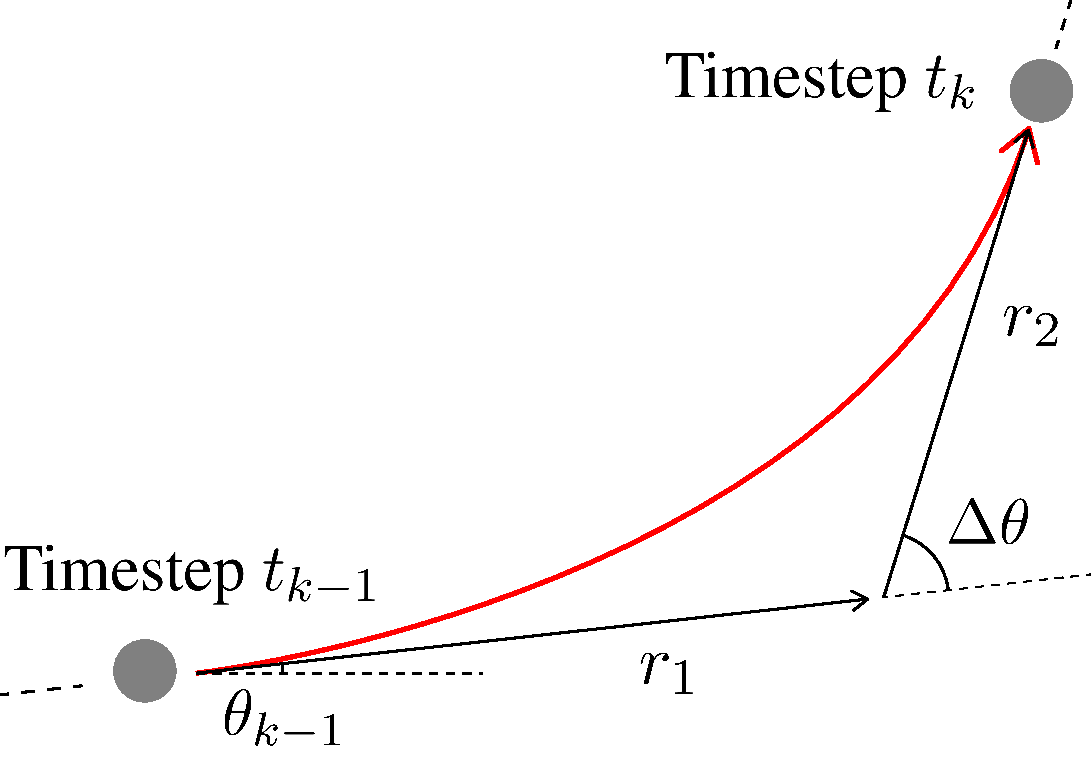
\includegraphics[width=0.5\columnwidth]{entity_move.pdf}
\caption{Illustrated movement of each entity in turn $k$.
}
\label{06_fig:entity_movement}
\end{figure}

To enable fair comparison with OCC, we limit the number of agents to 2 and set the circular agent views to have the same diameter as OCC. At each selection timestep $t_k$, we ensure that each agent has 7 observable entities with only 4, 5 or 6 of them in common, which is also identical to OCC. Finally, we sample all entity attributes (color, size and initial location) from the same uniform distributions as OCC with minimal modifications.\footnote{To be specific, we set the minimum distance between entities (at $t_k$) and the possible range of entity size to be slightly different to avoid entity overlapping during movements.} Therefore, we expect the (distribution of) observations at $t_k$ to be similar and enable mostly fair comparison with OCC (Sections \ref{06_sec:dataset_analysis} and \ref{06_sec:experiments}).

To ensure task difficulty, we also shift the \textit{perspective} of each agent after each successful turn (see Figure \ref{06_fig:first_example}) so that the overlapping regions differ every turn. The same dot is prohibited from staying in common for over 3 consecutive selection timesteps, requiring frequent updates of common ground. Finally, we limit the maximum number of turns to 5 for practical purposes (hence the maximum LST is 5 in each game).


\begin{figure*}[t!]
\centering
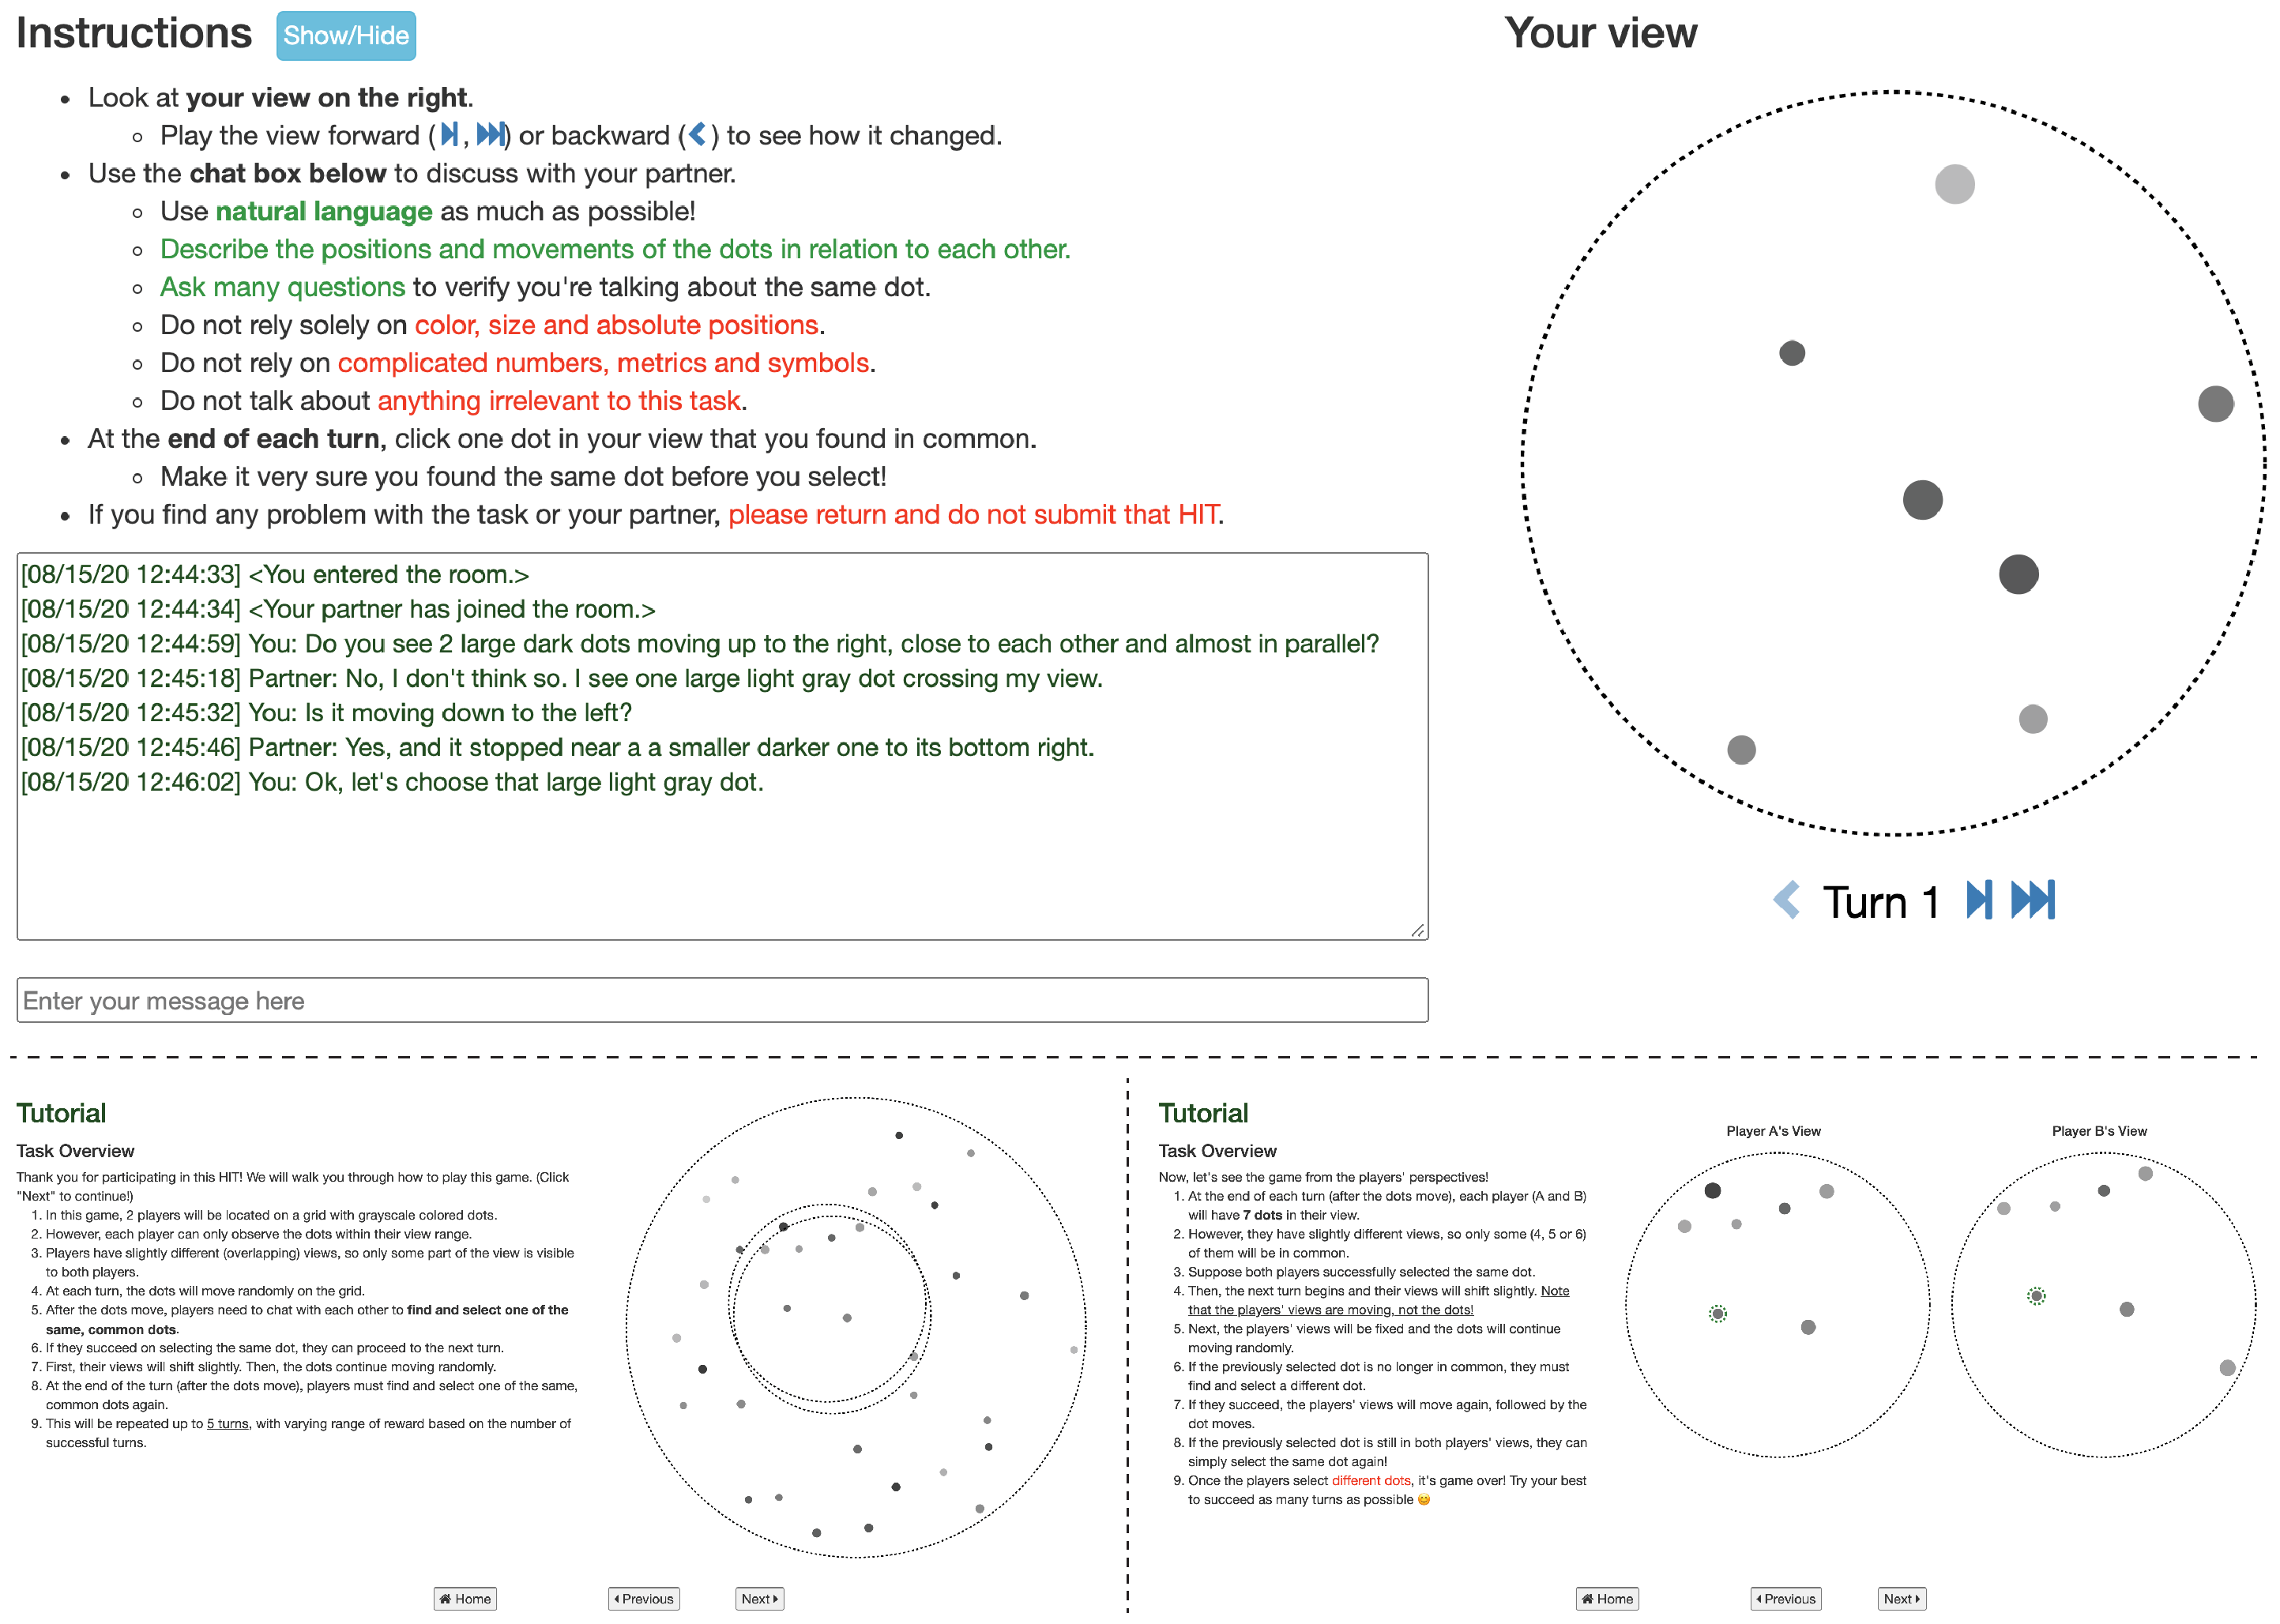
\includegraphics[width=\textwidth]{user_interfaces.pdf}
\caption{(Top) Our dialogue interface. During the game, animations up to the current turn could be replayed anytime using the forward/backward buttons. (Bottom) Sample screenshots from our tutorial on the \textit{task setting}.
}
\label{06_fig:user_interfaces}
\end{figure*}

\section{Dataset Collection}
\label{06_sec:dataset_collection}

To collect large-scale, high-quality dialogues, we conducted careful crowdsourcing on Amazon Mechanical Turk. The web application is based on the CoCoA framework \citep{he2017learning}, and we used Scalable Vector Graphics (SVG) to animate entity movements and parallel shifts of the agent perspectives. Before working on our task, crowd workers were required to take a brief tutorial on the task setting, dialogue interface and instructions. Sample screenshots of our dialogue interface and tutorial are shown in Figure \ref{06_fig:user_interfaces}: note that animations up to the current turn could be replayed anytime for the ease of playing the game.\footnote{This also allows us to ignore the disadvantage of imperfect human memories in comparison to machines.}

To ensure worker quality, we required crowd workers to have more than 500 completed HITs and acceptance rates higher than 99\%. To encourage success, we rewarded \$0.25 for every successful turn plus additional bonuses for longer LST achieved (up to \$0.25 if LST $=$ 5). Finally, we manually reviewed all submitted works and excluded dialogues which clearly violated the instructions (e.g. relying on premature guessing or other ineffective strategies\footnote{Typical examples include strategies relying solely on color, size and absolute positions in the agent's view.}). We did not exclude dialogues based on task failures (even if LST $=$ 0), as long as they were based on valid strategies.

To solicit linguistic/strategic variety, we generally used a unique environment for each game. However, if the task was unsuccessful (i.e. LST $=$ 0), we allowed the environment to be reused in another game. This way, we can expect to eventually collect successful (LST $>$ 0) dialogues for the relatively difficult environments as well.

Overall, we collected 5,804 dialogues, and after the reviewing process, we were left with 5,617 qualified dialogues. We refer to this dataset as \textbf{Dynamic-OneCommon Corpus (D-OCC)}. Note that our dataset is currently in English, but the dataset collection procedure is language-agnostic and can be applied in any other languages.


\section{Dataset Analysis}
\label{06_sec:dataset_analysis}

Next, we conduct detailed analyses of the dataset to study human common grounding strategies under dynamic context. Whenever possible, we give comparative analyses with OCC to highlight the effect of dynamic factors introduced in D-OCC.

\subsection{Overall Statistics}
\label{06_sec:overall_statistics}

\begin{table}[th!]
\centering \scalebox{0.85}{
\setlength\tabcolsep{8pt}
\begin{tabular}{lcc}
\toprule[\heavyrulewidth]
Statistics & OCC & D-OCC \\
\midrule
Total dialogues & 6,760 & 5,617 \\
Uttrances per dialogue & 4.8 & 11.7 \\
Tokens per utterance & 12.4 & 10.3 \\
Duration per dialogue (minutes) & 2.1 & 5.7 \\
Unique workers & N/A & 462 \\
Avg. LST & - & 3.31 \\
Avg. completed turns & - & 3.77 \\
\midrule
Unique tokens & 3,621 & 3,895 \\
Occupancy of rare tokens (\%) & 1.4 & 1.0 \\
Overlap of all tokens (\%) & \multicolumn{2}{c}{29.4} \\
Overlap w/o rare tokens (\%) & \multicolumn{2}{c}{53.0} \\
\bottomrule[\heavyrulewidth]
\end{tabular}
}
\caption{
Statistics of OCC and D-OCC datasets.
}
\label{06_tab:onecommon_statistics}
\end{table}

First, we summarize the overall statistics of OCC and D-OCC in Table \ref{06_tab:onecommon_statistics}.

In total, OCC and D-OCC have a comparable number of dialogues. However, dialogues can be much longer in D-OCC, since collaborative reference is repeated multiple times. On average, utterance lengths are slightly shorter in D-OCC: this can be attributed to the increased (relative) frequency of short utterances like acknowledgements and \textit{shortened} subsequent responses (e.g. ``same again?'' $=$ ``select the \underline{same} black dot \underline{again}?'').\footnote{In fact, utterances with less than 5 tokens were almost twice more frequent in D-OCC (33.8\%) than OCC (17.6\%).} Note that long, complex utterances are also common in our dataset, as seen in Figure \ref{06_fig:first_example}. Overall, we found 462 unique workers participated in D-OCC, which indicates reasonable diversity at the \textit{player} level as well.

In terms of LST, the overall average was 3.31 with over half (53.5\%) of the dialogues succeeding all 5 turns. This suggests that humans can solve the task reliably through sophisticated common grounding. After filtering dialogues with poor/careless workers (whose avg. LST $<$ 2), we observed a slight improvement up to 3.57. If we only focus on the top 10 workers (with at least 10 tasks completed), avg. LST was significantly higher reaching 4.24. These results indicate that (at least potentially) much higher human ceiling performance can be achieved. Note that if we include the unsuccessful turns in 46.5\% of the dialogues, the average of all completed turns was slightly longer (3.77) in our dataset.

Finally, we found that both datasets have a relatively small vocabulary size as well as the occupancy of \textit{rare tokens} (used less than 10 times in the dataset).\footnote{Occupancy is computed based on the proportion of total frequencies (TF), i.e. \textit{TF of rare tokens} / \textit{TF of all tokens}.} This indicates minimal complexity at the \textit{lexical} level, as observed in \citet{udagawa2019natural}. We also found that the two datasets have a large vocabulary overlap, which is expected as D-OCC extends the setting of OCC.


\begin{table*}[th]
\centering \scalebox{0.77}{
\setlength\tabcolsep{5pt}
\newcommand{\intermidrule}{\cmidrule{2-3}} 
\begin{tabular}{llc}
\toprule
\multicolumn{1}{c}{\multirow{2}{*}{\parbox{2cm}{Reference}}} & \multicolumn{1}{c}{\multirow{2}{*}{Examples}} & Frequency\\
 & & / Cohen's $\kappa$ \\
\midrule
\multirow{4}{*}{\parbox{2cm}{Current State}} &It's to the right of where the grey one \underline{ended up} for me \underline{after} moving up and left. & \multirow{4}{*}{\parbox{1cm}{23.8\% / 0.91}} \\
&\underline{Now} I have another triangle / Does it \underline{land} next to two smaller gray dots?& \\
&Does it have a lighter one below and to the left \underline{when they stop}?& \\
&Two similar shades close to each other (\textit{implicit})& \\
\midrule
\multirow{4}{*}{\parbox{2cm}{State Change}} &a small dark one \underline{traveling} southwest / 2 other dots \underline{following} it& \multirow{4}{*}{\parbox{1cm}{32.7\% / 0.97}} \\
&Do you have two dark med-size dots \underline{move slowly apart} as they \underline{drift} right? & \\
&I have a large pale grey that \underline{moves down} but starts out \underline{curving} to the right and & \\
&then \underline{takes a sharp turn} to the south east & \\
\midrule
\multirow{3}{*}{\parbox{2cm}{Previous State}} &I still see the larger gray one that \underline{was} next to it \underline{in the previous turn}. & \multirow{3}{*}{\parbox{1cm}{\phantom{0}5.5\% / 0.79}}\\
&I have the smaller dot that \underline{started out} below it to the left. & \\
&\underline{Before it moves}, is there a lighter gray dot down and to the right of it?& \\
\bottomrule
\end{tabular}
}
\caption{\label{06_tab:spatio_temporal_expressions}
Spatio-temporal expressions. Keywords (such as \textit{tense}, \textit{events} and \textit{motion verbs}) are underlined.
}
\end{table*}

\begin{table*}[th]
\centering \scalebox{0.83}{
\setlength\tabcolsep{9pt}
\setlength{\aboverulesep}{0pt}
\setlength{\belowrulesep}{0pt}
\setlength{\extrarowheight}{.4ex}
\begin{tabular}{c|cc|cl}
\toprule
Degree Modifiers & OCC & D-OCC & \# Keywords & \multicolumn{1}{l}{Usage in D-OCC} \\
\midrule
Diminishers & 9.2 & 8.9 & 10 & \textbf{slightly} curves up \\
Moderators & 1.3 & 0.9 & 6 & \textbf{fairly} quickly \\
Boosters & 9.8 & 6.1 & 27 & \textbf{extremely} slowly \\
Approximators & 10.2 & 6.4 & 34 & \textbf{almost} collides with \\
Maximizers & 4.3 & 4.2 & 37 & \textbf{perfectly} straight \\
\bottomrule
\end{tabular}
}
\caption{\label{06_tab:nuanced_expressions}
Average occurrences of degree modifiers per 100 utterances (estimated based on keywords).
}
\end{table*}


\subsection{Spatio-Temporal Expressions}
\label{06_subsec:spatio_temporal_expressions}

At the utterance level, we observed an extensive usage of \textit{spatio-temporal expressions} which are characteristic in dynamic environments. To study the frequency of such expressions, we manually annotated 100 dialogues in D-OCC with LST $\geq$ 2 (focusing on the more successful strategies).

Specifically, we detect whether each utterance contains 3 types of spatio-temporal expressions:\footnote{Note that a single utterance may contain none or multiple types of such expressions, and expressions of color, size or possession are not considered as spatio-temporal expressions.}

\begin{itemize}
    \item Reference to \textbf{current state} describes location of entities at the end of the current turn (i.e. timestep $t_k$ if the utterance is in turn $k$).
    \item Reference to \textbf{state change} describes temporal change of entity locations (i.e. movements).
    \item Reference to \textbf{previous state} describes entity locations at previous timestep $t$ (where $t < t_k$).
\end{itemize}

We show examples and estimated frequencies of spatio-temporal expressions in Table \ref{06_tab:spatio_temporal_expressions}. We also computed the agreement of our annotation based on 50 dialogues with 3 annotators, which we found to be reliable based on Cohen's $\kappa$ \citep{cohen1968weighted}.

Based on this result, we found that reference to \textit{state change} is the most widely used strategy, which could be simple as ``moves northwest'' or more complex as in Table \ref{06_tab:spatio_temporal_expressions}. Reference to \textit{previous state} is much less frequent compared to other types but still observed in many dialogues. Note that humans distinguish \textit{previous} and \textit{current} states in various ways, including temporal expressions (``was'', ``now''), motion verbs (``started out'', ``landed'') and implicit/default reasoning.

We also found that expressions are often \textit{nuanced} and \textit{pragmatic}, which are characteristic under continuous and partially-observable context \citep{udagawa2019natural}. 
Nuances are typically expressed by the \textit{degree modifiers} to convey subtle differences in location, movements, confidence, etc. Following \citet{paradis_2008}, we categorize them into 2 main types (and 5 subtypes): \textit{scalar modifiers} used for concepts in a range of scale (\textit{diminishers}, \textit{moderators}, \textit{boosters}) and \textit{totality modifiers} used for concepts with definite boundaries (\textit{approximators}, \textit{maximizers}). See Table \ref{06_tab:nuanced_expressions} for examples and the estimated occurrences of such modifiers in OCC and D-OCC.\footnote{Following the prior analysis in OCC, we manually curated keyword-based dictionaries of such modifiers (based on unigrams and bigrams) while removing polysemous words (such as \textit{little}, \textit{about}, \textit{too}, etc).} Based on these results, we can verify that there are comparable numbers of various degree modifiers in D-OCC as well, which are used effectively to cope with complex ambiguity and uncertainty.

\begin{figure}[t!]
\centering \small
\begin{tikzpicture}
\node[inner sep=0pt] (agent_0) at (0,0)
  {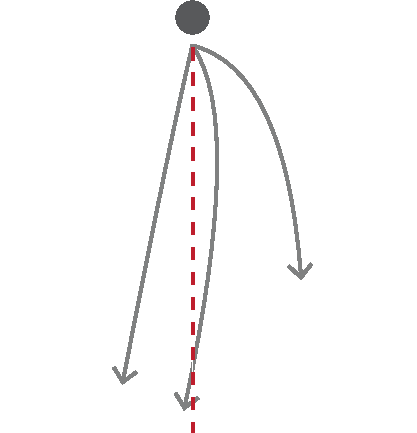
\includegraphics[width=0.27\columnwidth]{straight_down.pdf}};
\node[inner sep=0pt] (agent_1) at (4,0)
  {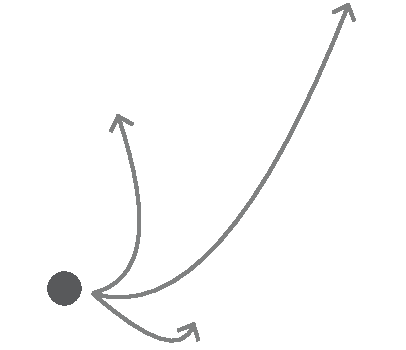
\includegraphics[width=0.27\columnwidth]{right_then_up.pdf}};
\node [below] at (0,-2.1) {straight down};
\node [below] at (4,-2.1) {right (and) then up};
\end{tikzpicture}
\caption{
Pragmatic expressions of movements.
}
\label{06_fig:pragmatic_movements}
\end{figure}

\begin{figure}[t!]
\vspace{3mm}
\centering \small
\begin{tikzpicture}
\node[inner sep=0pt] (fig_1) at (0,0)
  {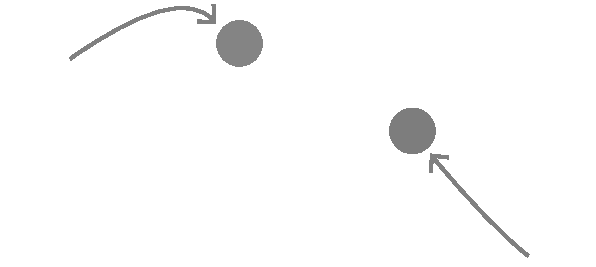
\includegraphics[width=0.28\columnwidth]{move_toward.pdf}};
\node[inner sep=0pt] (fig_2) at (4,0)
  {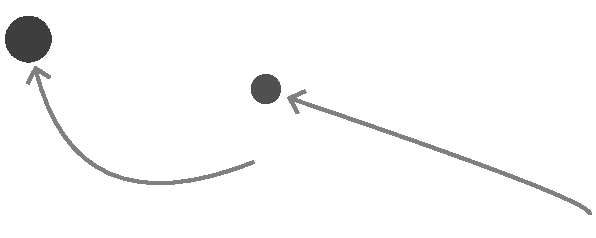
\includegraphics[width=0.28\columnwidth]{follow_behind.pdf}};
\node [below] at (0,-1) {\small toward each other};
\node [below] at (4.2,-1) {\small follow (behind)};
\node[inner sep=0pt] (fig_3) at (0,-3.3)
  {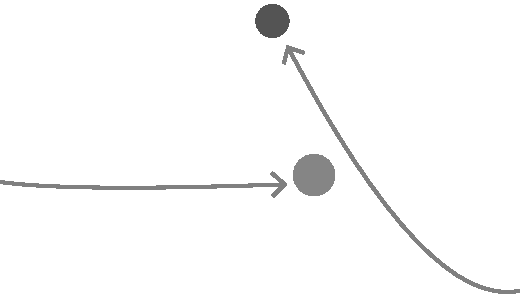
\includegraphics[width=0.26\columnwidth]{cross_in_front.pdf}};
 \node [below] at (0,-4.8) {\small cross in front};
 \node[inner sep=0pt] (fig_4) at (4,-3.3)
  {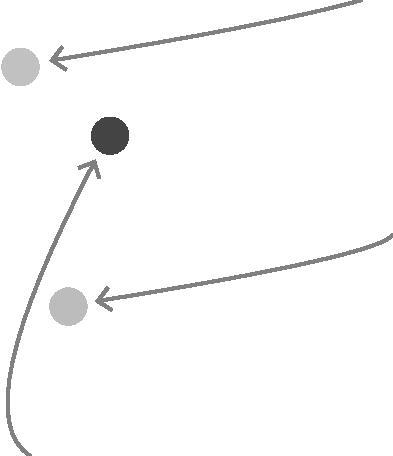
\includegraphics[width=0.18\columnwidth]{through_between.pdf}};
 \node [below] at (4,-4.8) {\small through (between)};
\end{tikzpicture}
\caption{
Expressions of multiple entity interactions.
}
\label{06_fig:entity_interactions}
\end{figure}

In Figure \ref{06_fig:pragmatic_movements}, we show examples of \textit{pragmatic} expressions which require pragmatic (non-literal) interpretations \citep{monroe2017colors}. For instance, trajectories of the expression ``straight down'' may not indicate vertical lines in the literal sense (e.g. could be curving or leaning to the left). Similarly, the expression of ``(moving) right and (then) up'' may be used for diverse movements ending up in various locations (e.g. even below the initial location!). While such expressions more or less deviate from literal semantics, they are pragmatically sufficient to convey the speaker's intention (i.e. identify the target among the distractors) \citep{Grice1975LogicAC}: alternatively, the speaker may need to choose different expressions for the same movement depending on the context (distractors).

We also show exemplary expressions of multiple entity interactions in Figure \ref{06_fig:entity_interactions}, which demonstrate interesting pragmaticality as well. For instance, ``toward each other'' may be used for trajectories moving in \textit{orthogonal} (rather than opposite) directions for the most of the time.

Overall, our analyses of spatio-temporal expressions reveal advanced language understanding and generation required in D-OCC, regardless of the task/lexical simplicity.


\begin{table*}[t!]
\centering \scalebox{0.82}{
\setlength\tabcolsep{7pt}
\setlength{\aboverulesep}{0pt}
\setlength{\belowrulesep}{0pt}
\setlength{\extrarowheight}{.4ex}
\newcommand{\intermidrule}{\cmidrule{2-8}}
\newcommand{\intermidmidrule}{\cmidrule{2-8}} 
\begin{tabular}{ccc|ccccc}
\toprule
\multirow{2}{*}{Dataset} & \multirow{2}{*}{Turn} & \raisebox{-1pt}{Previous} & \multicolumn{3}{c}{\raisebox{-1pt}{Success Rate (\%)}} & \raisebox{-1pt}{Utterances} & \raisebox{-1pt}{Tokens per} \\
 & & \raisebox{1pt}{Target} & \raisebox{1pt}{\#Shared=4} & \raisebox{1pt}{\#Shared=5} & \raisebox{1pt}{\#Shared=6} & \raisebox{1pt}{per Turn} & \raisebox{1pt}{Utterance} \\
\midrule
OCC & \nth{1} & - & 65.8 & 77.0 & 87.0 & 4.8 & 12.4 \\
\midrule
\multirow{3}{*}{D-OCC} & \nth{1} & - & 73.4 & 82.0 & 87.6 & 3.2 & 11.0 \\
 & \multirow{2}{*}{$\geq$\nth{2}} & \cmark & 95.4 & 97.0 & 97.8 & 2.3 & \phantom{0}5.9 \\
 & & \xmark & 81.7 & 88.4 & 91.6 & 3.5 & 11.7 \\
\bottomrule
\end{tabular}
}
\caption{\label{06_tab:turn_level_statistics}
Turn-level statistics of OCC and D-OCC. \,\cmark\,denotes cases where the previous target stays in common and \,\xmark\,denotes it left at least one agent's view. Note that \# shared entities are 4, 5 or 6 at selection timesteps (Section \ref{06_subsec:sequential_collaborative_reference_task}).
}
\end{table*}

\begin{table*}[t!]
\centering \scalebox{0.83}{
\setlength\tabcolsep{8pt}
\begin{tabular}{clc}
\toprule
\multicolumn{1}{c}{Previous} & \multicolumn{1}{c}{\multirow{2}{*}{Examples}} & \multirow{2}{*}{Frequency (\%)} \\
\multicolumn{1}{c}{Target} & & \\
\midrule
\multirow{3}{*}{Stay (\cmark)} & I still see the same dot / same one again? & \multirow{3}{*}{36.8} \\
& I still have all three dots from the line before & \\
& Left my screen, but may have come back traveling left to right? &  \\
\midrule
\multirow{3}{*}{Leave (\xmark)} & I lost the last one / both are gone for me & \multirow{3}{*}{63.2} \\
& I lost the light one but still see the darker one that was on its left. & \\
& similar size black dot that barely moves? (\textit{implicit}) & \\
\bottomrule
\end{tabular}
}
\caption{\label{06_tab:turn_level_utterances}
Comparison of utterances when the previous target stays in common (\cmark) or not (\xmark).
}
\end{table*}

\subsection{Turn-Level Strategies}
\label{06_subsec:turn_level_strategies}

Finally, we study and compare human strategies at different timesteps (in different turns). Table \ref{06_tab:turn_level_statistics} shows detailed statistics of the dataset in the initial turn and later turns, where \textit{creation} and \textit{maintenance} of common ground are required, respectively. Note that we also distinguish later turns based on whether the previous selection (i.e. \textit{previous target}) stays in common (\cmark) or leaves at least one agent's view (\xmark): former cases can \textit{retain} the same common ground but the latter cases require an \textit{update} of common ground.

First, if we focus on the \nth{1} turn, we can verify that success rates are consistently higher in D-OCC than OCC, especially in difficult cases when the number of shared entities is smaller. This indicates that humans can create common ground more accurately by leveraging dynamic information (e.g. entity movements) unavailable in OCC.

In later turns, we found that human performance is near perfect with shorter dialogues in \cmark\,cases (when the previous target stays in common). This is natural because they can simply retain common ground and repeat the same selection. Notably, human performance is consistently higher than the \nth{1} turn \textit{even in} \xmark\,cases (when the previous target is no longer in common), which verifies that humans can leverage previous common ground to \textit{update} common ground more reliably as well.

We show example utterances of \cmark\,and \xmark\,cases in Table \ref{06_tab:turn_level_utterances}. Note that the previous target may temporarily leave the view and come back in \cmark\,cases, which occasionally makes even \textit{retainment} of the same common ground non-trivial. In \xmark\,cases, humans either inform about the lost entities explicitly or \textit{implicitly}, e.g. by ignoring old entities and starting to focus on the new ones.


\section{Experiments}
\label{06_sec:experiments}

Finally, we conduct extensive experiments to assess our baseline model's capability of common grounding in dynamic environments.

\subsection{Evaluation}
\label{06_subsec:evaluation}

To study the model's capability from various aspects, we design 3 (sub)tasks based on D-OCC.

First, we evaluate the model's ability of \textit{recognizing} common ground based on the \textbf{target selection task}, originally proposed for OCC. This is an important subtask of (sequential) collaborative reference, where the model is given one player's observation and the (ground-truth) dialogue history to predict which target was selected by the player. Since there can be multiple selections in D-OCC, the model makes predictions at the end of each turn $k$ (at timestep $t_k$). The number of entities observable at $t_k$ is fixed at 7 for both OCC and D-OCC (Section \ref{06_subsec:sequential_collaborative_reference_task}), so this is a simple classification task evaluated based on accuracy.

Secondly, we estimate the model's ability of \textit{creating} and \textit{maintaining} common ground based on the \textbf{selfplay dialogue task}, where each model plays the full sequential collaborative reference task against an identical copy of itself. While this evaluation has the advantage of being scalable and automatic, succeeding on this setting is only \textit{necessary} for human-level common grounding and not \textit{sufficient}, since the model may only be able to coordinate with itself (and not with real humans).

Thirdly, we conduct \textbf{human evaluation} to test the model's ability of playing sequential collaborative reference against real human workers on AMT. Due to the high cost of this evaluation, we only focus on the top 3 variants of our baseline ranked by avg. LST in the selfplay dialogue task.

\subsection{Model Architecture}
\label{06_subsec:model}

For a fair comparison with prior work, we implement our baseline model following the OCC models in \citet{udagawa2020annotated}. The overall model architecture is shown in Figure \ref{06_fig:model_architecture}.

To encode the dialogue tokens throughout the turns, we use a unidirectional GRU \citep{cho2014properties}. To encode the observation during turn $k$, we first split the animation of entity movements into 10 frames and the agent view shift into 5 frames. Then, we process each observation frame based on the \textit{spatial} encoder, followed by the \textit{temporal} encoder to integrate these outputs.

The spatial encoder is used to extract \textit{spatial features} and \textit{meta features} from each observation frame. Spatial features represent the spatial attributes of each entity (color, size and location in the frame), which are encoded using an MLP and a relation network \citep{santoro2017simple}. The relation network is used to represent the spatial attributes relative to a subset of entities $\tilde{E} \subset E$, which could be \textit{all entities} observable in turn $k$ ($E_{all}$) or \textit{selectable entities} visible at $t_k$ ($E_{sel}$). Hence, the spatial features of $e_i$ are computed as:
%
\begin{equation}\label{eqt:spatial_features}
\mathrm{MLP}(\mathbf{e}_i) \odot \sum_{\substack{e_j \in \tilde E, \\ j \neq i }} \mathrm{MLP}(\mathbf{e}_i - \mathbf{e}_j)
\end{equation}
%
where  $\mathbf{e}_i$ is the vector representation of entity $e_i$ and $\odot$ is the vector concatenation.\footnote{To be precise, $\mathbf{e}_i$ is a 4-dimensional vector representing color, size, and 2-D location. If the entity is not observable in the frame, we use the default value of (0, 0) for the location.}

Meta features are binary information of each entity representing whether (or not) the entity (i) is visible in the frame, (ii) is visible at timestep $t_{k}$, (iii) was visible at timestep $t_{k-1}$, and (iv) was selected in the previous turn (i.e. is the \textit{previous target}). Meta features are also encoded using an MLP, and we take the sum of spatial/meta features as the (entity-level) output of the spatial encoder.

Finally, we use the temporal encoder based on a GRU to encode the outputs of the spatial encoder. The final state of the temporal encoder is considered as the final representation of each entity.

Based on the outputs of these encoders, we use two attention modules (based on MLPs) to compute attention scores for each entity. The first attention module is used to weight the final representations of all entities $E_{all}$ conditioned on the current dialogue state: then, the weighted sum of $E_{all}$ is concatenated with the dialogue state to predict the next dialogue token \citep{xu2015show}. The second module is used to predict the target entity, where we simply take the (soft)max of attention scores for the selectable entities $E_{sel}$ in turn $k$.

Note that there are only two main differences between our baseline and the best OCC model (TSEL-REF-DIAL) from \citet{udagawa2020annotated}: first, in TSEL-REF-DIAL, the final representation of each entity is its \textit{spatial features}, i.e. the meta features and temporal encoder are not used (which are only meaningful in D-OCC). Second, TSEL-REF-DIAL is also trained on the \textit{reference resolution} task (using an additional attention module), which is only available in OCC. Due to this architectural similarity, we can virtually \textit{pretrain} our model on OCC by initializing the shared model parameters based on TSEL-REF-DIAL and then fine-tune the whole model on D-OCC.\footnote{For pretraining, we retrained TSEL-REF-DIAL with the shared word embedding for OCC and D-OCC.}

\begin{figure*}[tb!]
\centering
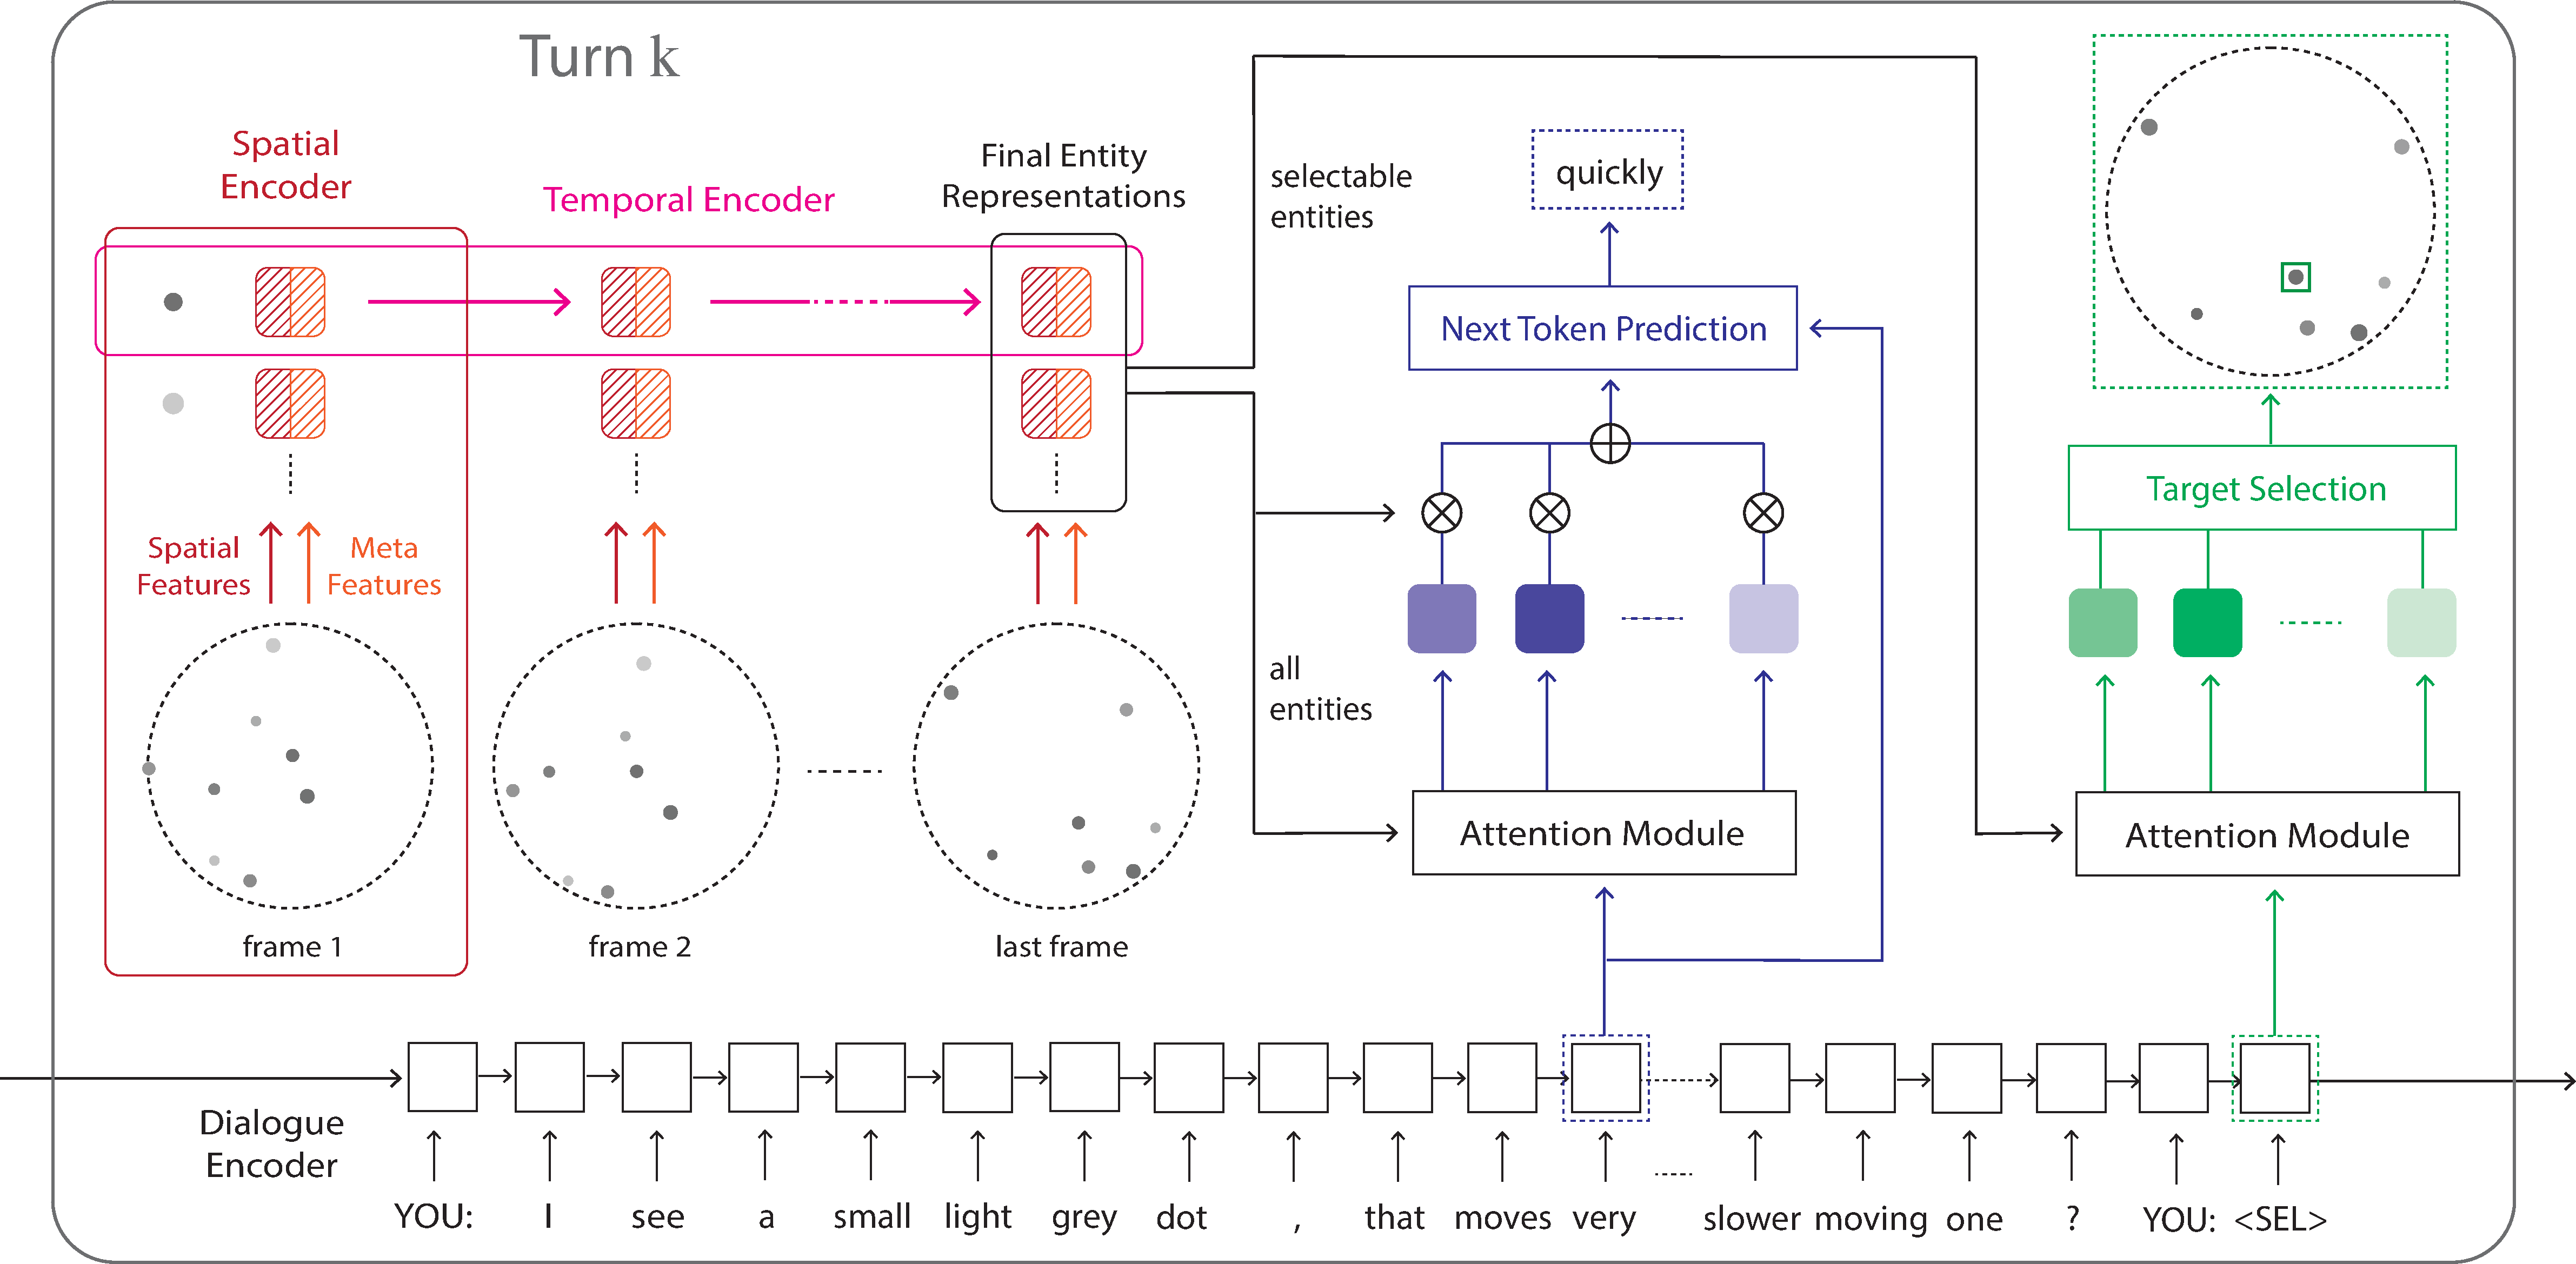
\includegraphics[width=\textwidth]{overall_model_architecture.pdf}
\caption{Our baseline model architecture. Information flow in turn $k$ is illustrated.
When generating model utterances (in selfplay dialogue and human evaluation), we sample next tokens with the temperature set to 0.25.
}
\label{06_fig:model_architecture}
\end{figure*}

\subsection{Experiment Setup}
\label{06_subsec:experiment_setup}

All modules of our baseline (MLPs and GRUs) are single layered with 256 hidden units, except for the attention modules which are 2-layered. Dropout rate of 0.5 is applied at each layer during training, and we use the Adam optimizer \citep{Kingma2015AdamAM} with the initial learning rate set to 0.001. After manual tuning on the validation set, we weight the losses from next token prediction and target selection with the ratio of 2:1.

In terms of data splits, we use 500 dialogues with LST $\geq$ 2 for testing target selection, another 500 for validation and the rest for training.\footnote{We ensured no overlaps in terms of the \textit{environments} across data splits.} Note that we use all unsuccessful turns (where the players failed to agree upon the same entity) as well, assuming they are still based on valid strategies. For selfplay dialogue and human evaluation, we collect 2,000 and 200 dialogues in unseen environments, respectively. Each experiment is repeated 5 times with different random seeds (including data splits), except for human evaluation.

Finally, we conduct extensive ablations to study the effect of various model architectures, including \textit{pretraining}, spatial attributes (\textit{color}, \textit{size} and \textit{location}) and the meta feature (\textit{previous target}). In addition, we also ablate the \textit{dynamic} information of the observation by only using the last frame in each turn as the input for the temporal encoder.

\subsection{Results}
\label{06_subsec:results}

\begin{table}[ht]
\centering
\scalebox{0.83}{
\setlength\tabcolsep{6pt}
\begin{tabular}{lccc}
\toprule
\multirow{2}{*}[-0.8ex]{Model}& \multicolumn{3}{c}{Turn / Previous Target} \\
\cmidrule{2-4}
 & \nth{1} / - & $\geq$\nth{2} / \cmark & $\geq$\nth{2} / \xmark \\
\midrule
Baseline & \textbf{76.4{\scriptsize $\pm$1.7}} & 96.6{\scriptsize $\pm$0.3}\phantom{$^*$} & 67.4{\scriptsize $\pm$0.5}\phantom{$^*$} \\
\phantom{F}$-$ pretraining & 74.6{\scriptsize $\pm$2.7} & 96.3{\scriptsize $\pm$0.7}\phantom{$^*$} & 66.9{\scriptsize $\pm$1.1}\phantom{$^*$} \\
\phantom{F}$-$ color & 56.3{\scriptsize $\pm$2.0} & 95.7{\scriptsize $\pm$0.6}\phantom{$^*$} & 50.5{\scriptsize $\pm$1.4}\phantom{$^*$} \\
\phantom{F}$-$ size & 58.4{\scriptsize $\pm$1.3} & 95.7{\scriptsize $\pm$0.9}\phantom{$^*$} & 52.2{\scriptsize $\pm$0.5}\phantom{$^*$} \\
\phantom{F}$-$ location & 74.4{\scriptsize $\pm$1.5} & 96.1{\scriptsize $\pm$0.9}\phantom{$^*$} & 67.3{\scriptsize $\pm$0.7}\phantom{$^*$} \\
\phantom{F}$-$ previous target & 76.1{\scriptsize $\pm$1.7} & 83.3{\scriptsize $\pm$1.1}$^*$ & \textbf{67.8{\scriptsize $\pm$0.6}}$^*$ \\
\phantom{F}$-$ dynamics & 75.1{\scriptsize $\pm$2.3} & \textbf{96.7{\scriptsize $\pm$1.0}}\phantom{$^*$} & 67.0{\scriptsize $\pm$0.7}\phantom{$^*$} \\
\midrule
Human & 97.0{\scriptsize $\pm$1.1} & 98.2{\scriptsize $\pm$0.5}$^*$ & 95.8{\scriptsize $\pm$2.0}$^*$ \\
\bottomrule
\end{tabular}
}
\caption{\label{06_tab:model_target_selection}
Results for the target selection task ($^*$ denotes cases where the correct previous targets were not provided during prediction).
}
\end{table}

\begin{table*}[th!]
\centering
\scalebox{0.77}{
\setlength\tabcolsep{7pt}
\setlength{\aboverulesep}{0pt}
\setlength{\belowrulesep}{0pt}
\setlength{\extrarowheight}{.1ex}
\newcommand{\intermidrule}{\cmidrule{2-8}}
\newcommand{\intermidmidrule}{\cmidrule{2-8}} 
\begin{tabular}{l|ccc|cccc}
\toprule
\multicolumn{1}{c}{} & & & \multicolumn{1}{c}{} & \multicolumn{4}{|c}{\textbf{Seflplay Dialogue}} \\
\midrule
\midrule
\multirow{2}{*}{Model}& \multirow{2}{*}{Dataset} & \multirow{2}{*}{Turn} & \raisebox{-0.5pt}{Previous} & \multicolumn{3}{c}{\raisebox{-0.5pt}{Success Rate (\%)}} & \raisebox{-0.5pt}{Avg.} \\
 & & & \raisebox{0.5pt}{Target} & \raisebox{0.5pt}{\#Shared=4} & \raisebox{0.5pt}{\#Shared=5} & \raisebox{0.5pt}{\#Shared=6} & \raisebox{0.5pt}{LST} \\
\midrule
\multirow{3}{*}{Baseline} & \multirow{3}{*}{D-OCC} & \nth{1} & - & 46.8{\scriptsize $\pm$1.8} & 63.8{\scriptsize $\pm$1.8} & 80.2{\scriptsize $\pm$2.3} & \multirow{3}{*}{1.94{\scriptsize $\pm$0.09}} \\
 & & \multirow{2}{*}{$\geq$\nth{2}} & \cmark & 99.4{\scriptsize $\pm$0.3} & 99.7{\scriptsize $\pm$0.2} & 99.6{\scriptsize $\pm$0.2} & \\
 & & & \xmark & \textbf{48.5{\scriptsize $\pm$2.2}} & \textbf{64.6{\scriptsize $\pm$2.8}} & \textbf{81.5{\scriptsize $\pm$1.5}} & \\
\midrule
\multirow{3}{*}{\phantom{F}$-$ pretraining} & \multirow{3}{*}{D-OCC} & \nth{1} & - & 39.4{\scriptsize $\pm$1.0} & 53.5{\scriptsize $\pm$0.8} & 73.7{\scriptsize $\pm$1.8} & \multirow{3}{*}{1.35{\scriptsize $\pm$0.09}} \\
 & & \multirow{2}{*}{$\geq$\nth{2}} & \cmark & 98.6{\scriptsize $\pm$2.4} & 98.8{\scriptsize $\pm$1.8} & 99.4{\scriptsize $\pm$1.0} & \\
 & & & \xmark & 30.3{\scriptsize $\pm$5.7} & 42.1{\scriptsize $\pm$6.3} & 65.4{\scriptsize $\pm$4.9} & \\
\midrule
\multirow{3}{*}{\phantom{F}$-$ color} & \multirow{3}{*}{D-OCC} & \nth{1} & - & 36.3{\scriptsize $\pm$2.0} & 54.6{\scriptsize $\pm$2.3} & 72.9{\scriptsize $\pm$1.5} & \multirow{3}{*}{1.50{\scriptsize $\pm$0.10}} \\
 & & \multirow{2}{*}{$\geq$\nth{2}} & \cmark & 99.7{\scriptsize $\pm$0.1} & 99.7{\scriptsize $\pm$0.0} & 99.6{\scriptsize $\pm$0.1} & \\
 & & & \xmark & 42.1{\scriptsize $\pm$3.5} & 56.7{\scriptsize $\pm$4.2} & 72.4{\scriptsize $\pm$4.6} & \\
\midrule
\multirow{3}{*}{\phantom{F}$-$ size} & \multirow{3}{*}{D-OCC} & \nth{1} & - & 41.5{\scriptsize $\pm$0.8} & 58.0{\scriptsize $\pm$0.9} & 75.2{\scriptsize $\pm$1.3} & \multirow{3}{*}{1.58{\scriptsize $\pm$0.07}} \\
 & & \multirow{2}{*}{$\geq$\nth{2}} & \cmark & 99.8{\scriptsize $\pm$0.1} & 99.7{\scriptsize $\pm$0.1} & 99.8{\scriptsize $\pm$0.2} & \\
 & & & \xmark & 39.6{\scriptsize $\pm$3.5} & 55.3{\scriptsize $\pm$3.6} & 69.9{\scriptsize $\pm$1.5} & \\
\midrule
\multirow{3}{*}{\phantom{F}$-$ location} & \multirow{3}{*}{D-OCC} & \nth{1} & - & 45.7{\scriptsize $\pm$1.9} & 60.4{\scriptsize $\pm$1.6} & 77.7{\scriptsize $\pm$1.7} & \multirow{3}{*}{1.68{\scriptsize $\pm$0.09}} \\
 & & \multirow{2}{*}{$\geq$\nth{2}} & \cmark & 99.8{\scriptsize $\pm$0.1} & 99.7{\scriptsize $\pm$0.0} & 99.7{\scriptsize $\pm$0.1} & \\
 & & & \xmark & 40.8{\scriptsize $\pm$3.6} & 54.6{\scriptsize $\pm$2.5} & 73.9{\scriptsize $\pm$4.2} & \\
\midrule
\multirow{3}{*}{\phantom{F}$-$ previous target} & \multirow{3}{*}{D-OCC} & \nth{1} & - & \textbf{49.2{\scriptsize $\pm$1.3}} & 64.0{\scriptsize $\pm$1.8} & 82.2{\scriptsize $\pm$2.0} & \multirow{3}{*}{1.45{\scriptsize $\pm$0.05}} \\
 & & \multirow{2}{*}{$\geq$\nth{2}} & \cmark & 85.8{\scriptsize $\pm$2.7} & 87.5{\scriptsize $\pm$1.6} & 91.2{\scriptsize $\pm$1.3} & \\
 & & & \xmark & 29.2{\scriptsize $\pm$1.5} & 41.9{\scriptsize $\pm$1.9} & 64.5{\scriptsize $\pm$1.0} & \\
\midrule
\multirow{3}{*}{\phantom{F}$-$ dynamics} & \multirow{3}{*}{D-OCC} & \nth{1} & - & \textbf{49.2{\scriptsize $\pm$2.2}} & \textbf{65.8{\scriptsize $\pm$1.3}} & \textbf{83.3{\scriptsize $\pm$1.9}} & \multirow{3}{*}{\textbf{2.02{\scriptsize $\pm$0.07}}} \\
 & & \multirow{2}{*}{$\geq$\nth{2}} & \cmark & \textbf{99.9{\scriptsize $\pm$0.1}} & \textbf{99.9{\scriptsize $\pm$0.1}} & \textbf{99.8{\scriptsize $\pm$0.1}} & \\
 & & & \xmark & 48.3{\scriptsize $\pm$2.2} & 63.5{\scriptsize $\pm$2.8} & 81.1{\scriptsize $\pm$2.1} & \\
\midrule
\multirow{2}{*}{TSEL-REF-DIAL} & D-OCC & \nth{1} & - & 41.0{\scriptsize $\pm$1.2} & 58.7{\scriptsize $\pm$1.1} & 76.0{\scriptsize $\pm$1.8} & \multirow{2}{*}{-} \\
& OCC & \nth{1} & - & 45.9{\scriptsize $\pm$1.6} & 62.7{\scriptsize $\pm$2.2} & 79.7{\scriptsize $\pm$1.0} & \\
\midrule
\midrule
\multirow{3}{*}{Human} & \multirow{3}{*}{D-OCC} & \nth{1} & - & 73.4 & 82.0 & 87.6 & \multirow{3}{*}{3.31} \\
 & & \multirow{2}{*}{$\geq$\nth{2}} & \cmark & 95.4 & 97.0 & 97.8 & \\
 & & & \xmark & 81.7 & 88.4 & 91.6 & \\
\bottomrule
\end{tabular}
}
\caption{\label{06_tab:model_selfplay_dialogue}
Results for the selfplay dialogue task. Human performance is estimated based on the overall average of the crowd workers (c.f. Table \ref{06_tab:onecommon_statistics} and \ref{06_tab:turn_level_statistics}).
}
\end{table*}

\begin{table*}[th!]
\centering
\scalebox{0.77}{
\setlength\tabcolsep{7pt}
\setlength{\aboverulesep}{0pt}
\setlength{\belowrulesep}{0pt}
\setlength{\extrarowheight}{.1ex}
\newcommand{\intermidrule}{\cmidrule{2-8}}
\newcommand{\intermidmidrule}{\cmidrule{2-8}} 
\begin{tabular}{l|ccc|cccc|cc}
\toprule
\multicolumn{1}{c}{} & & & \multicolumn{1}{c}{} & \multicolumn{2}{|c}{\textbf{Human Evaluation}} \\
\midrule
\midrule
\multirow{2}{*}{Model}& \multirow{2}{*}{Dataset} & \multirow{2}{*}{Turn} & \raisebox{-0.5pt}{Previous} & \raisebox{-0.5pt}{\phantom{}Success\phantom{(}} & \raisebox{-0.5pt}{Avg.} \\
 & & & \raisebox{0.5pt}{Target} & \raisebox{0.5pt}{Rate (\%)} & \raisebox{0.5pt}{LST} \\
\midrule
\multirow{3}{*}{Baseline} & \multirow{3}{*}{D-OCC} & \nth{1} & - & \textbf{44.5} & \multirow{3}{*}{\textbf{1.00}} \\
 & & \multirow{2}{*}{$\geq$\nth{2}} & \cmark & 81.9 & \\
 & & & \xmark & \textbf{44.4} & \\
\midrule
\multirow{3}{*}{\phantom{F}$-$ location} & \multirow{3}{*}{D-OCC} & \nth{1} & - & 40.0 & \multirow{3}{*}{0.81} \\
 & & \multirow{2}{*}{$\geq$\nth{2}} & \cmark & \textbf{91.8} & \\
 & & & \xmark & 36.3 & \\
\midrule
\multirow{3}{*}{\phantom{F}$-$ dynamics} & \multirow{3}{*}{D-OCC} & \nth{1} & - & 37.0 & \multirow{3}{*}{0.79} \\
 & & \multirow{2}{*}{$\geq$\nth{2}} & \cmark  & 86.8 & \\
 & & & \xmark & 39.2 & \\
\midrule
\midrule
\multirow{3}{*}{Human} & \multirow{3}{*}{D-OCC} & \nth{1} & - & 80.5 & \multirow{3}{*}{3.31} \\
 & & \multirow{2}{*}{$\geq$\nth{2}} & \cmark & 96.7 & \\
 & & & \xmark & 86.6 & \\
\bottomrule
\end{tabular}
}
\caption{\label{06_tab:model_human_evaluation}
Results for the human evaluation. Human performance is estimated based on the overall average of the crowd workers (c.f. Table \ref{06_tab:onecommon_statistics} and \ref{06_tab:turn_level_statistics}).
}
\end{table*}


We show the results for target selection in Table \ref{06_tab:model_target_selection}. The human performance is estimated by 3 annotators based on 50 dialogues with LST $\geq$ 2.

Based on these results, we can verify that all ablations hurt the performance of our baseline in some way. Pretraining on OCC is generally effective, and all spatial attributes contribute to the overall performance (especially color and size). When the meta feature of the correct previous target is available, all models perform remarkably well in \cmark\,cases (previous target stays in common), which is natural since humans often repeated the same selection. Finally, dynamic information also contributes to the baseline performance, despite the effect being rather marginal.

However, there is huge room left for improvement in the \nth{1} turn and even more so in \xmark\,cases (previous target no longer in common). These results indicate that recognizing the \textit{creation} of common ground is still difficult, and recognizing how they are \textit{updated} (rather than \textit{retained}) remains even more challenging for the current baseline.

Next, we show the results for selfplay dialogue and human evaluation in Tables \ref{06_tab:model_selfplay_dialogue} and \ref{06_tab:model_human_evaluation}, respectively. We also include the results of TSEL-REF-DIAL (trained on OCC \textit{without} fine-tuning on D-OCC) as a reference.\footnote{When testing TSEL-REF-DIAL on D-OCC, we used the spatial features of the last observation frame as the input.}

In selfplay dialogue, we can verify that the baseline model performs reasonably well, outperforming TSEL-REF-DIAL in the \nth{1} turn of D-OCC (as well as OCC). However, it is worth noting that TSEL-REF-DIAL may be suffering from a minor covariate shift in D-OCC (c.f. Section \ref{06_subsec:sequential_collaborative_reference_task}), and without pretraining, our baseline still underperforms this best OCC model. We also found that all ablations of spatial attributes hurt performance, while the locational attributes became more critical in the full dialogue task. The meta feature of the previous target (selected by the model) is also critical, as the models seem to be relying heavily on this feature to both retain and update the target.

However, we found that ablation of dynamic information does not degrade (actually improves) performance in selfplay dialogue. This indicates that the last frame of each turn (\textit{current state}) is sufficient for the baseline to coordinate with itself, and it is unlikely to be leveraging sophisticated temporal information (\textit{state change} or \textit{previous state}) like the human strategies seen in Section \ref{06_subsec:spatio_temporal_expressions}. Also, while the models perform near perfectly in \cmark\,cases, the success rates drop or do not improve significantly in \xmark\,cases (compared to the \nth{1} turn). This shows that current models can \textit{retain} the same common ground easily but struggle in \textit{updating} them using the previous common ground, unlike the human strategies seen in Section \ref{06_subsec:turn_level_strategies}.

Finally, in human evaluation, we could verify that our baseline performs the best of the top 3 models in the selfplay dialogue task, but the success rates were much lower than observed in selfplay. This indicates that current models may not be using natural language in the same way humans use it (i.e. are not properly \textit{grounded}, \citealp{bender-koller-2020-climbing}), although they do become closer to it when all the features are available.\footnote{At the \textit{superficial} level, all models could generate fluent utterances and complete the task with minimal confusion.}

To summarize, our results in sequential collaborative reference show that the current baseline can leverage all spatial features and retain the same common ground, especially when provided explicitly as the meta feature. However, it may not be using temporal information effectively, and the creation and update of common ground still remain challenging in the dynamic environments, especially when conversing with real humans.

\section{Related Work}
\label{06_sec:related_work}

\begin{table*}[t!]
\centering \scalebox{0.67}{
\setlength\tabcolsep{6pt}
\begin{tabular}{ccccccc}
\toprule[\heavyrulewidth]
\multirow{2}{*}[-0.8ex]{\textbf{Dataset}} & \multicolumn{3}{c}{\textbf{Context Type}} & \raisebox{-2pt}{\textbf{Context}} & \raisebox{-2pt}{\textbf{Context}} & \raisebox{-2pt}{\textbf{Evaluation of}} \\
\cmidrule(r){2-4}
& \textbf{CNT} & \textbf{P.O.} & \textbf{DYN} & \raisebox{2pt}{\textbf{Update}} & \raisebox{2pt}{\textbf{Source}} & \raisebox{2pt}{\textbf{Common Grounding}} \\
\midrule
Twitch-FIFA \citep{pasunuru-bansal-2018-game} & \cmark & \xmark & \cmark & \cmark & Synthetic & N/A \\
AVSD \citep{alamri2019audio} & \cmark & \cmark & \cmark & \xmark & Real & Indirect \\
SIMMC \citep{moon-etal-2020-situated} & \cmark & \xmark & \xmark & \cmark & Synthetic+Real & Indirect \\
MutualFriends \citep{he2017learning} & \xmark & \cmark & \xmark & \xmark & Synthetic & Create \\
GuessWhat?! \citep{de2017guesswhat} & \cmark & \xmark & \xmark & \xmark & Real & Create \\
Photobook Dataset \citep{haber-etal-2019-photobook} & \cmark & \cmark & \xmark & \cmark & Real & Create \\
OneCommon \citep{udagawa2019natural} & \cmark & \cmark & \xmark & \xmark & Synthetic & Create \\
\midrule
\textbf{Dynamic-OneCommon (Ours)} & \cmark & \cmark & \cmark & \cmark & \textbf{Synthetic} & \textbf{Create+Maintain} \\
\bottomrule[\heavyrulewidth]
\end{tabular}
}
\caption{
Comparison with the major datasets. Context type is considered \textit{dynamic} if it involves rich, spontaneous dynamics (as in videos) and contexts to be \textit{updated} if new information is provided in the course of the dialogue (CNT = \textit{continuous}, P.O. = \textit{partially-observable}, DYN = \textit{dynamic}).
}
\label{tab:dataset_comparison}
\end{table*}

The notion of common ground was originally introduced in \citet{lewis1969convention} and \citet{stalnaker1978assertion} and theoretically elaborated in fields such as psycholinguistics \citep{clark1991grounding,brennan2010two}. While formal approaches (rule/logic-based) exist to computationally model the process of common grounding \citep{traum1994computational,van2007dynamic,poesio2010completions}, capturing their full complexities in realistic, situated conversations remains a formidable problem.

From an empirical perspective, various dialogue tasks have been proposed to develop and evaluate data-driven models of common grounding. Most of the existing literature focuses on closed domain, goal-oriented settings to measure the ability both quantitatively and objectively \citep{fang2015embodied,zarriess-etal-2016-pentoref,de2017guesswhat}. Recent works, summarized as the \textit{grounded agreement games} in \citet{schlangen2019grounded}, introduce symmetric speaker roles to encourage more bilateral interaction. \citet{udagawa2019natural} also raise \textit{continuous} and \textit{partially-observable} context to be essential for requiring advanced common grounding (Section \ref{06_subsec:collaborative_reference_task}). Finally, \citet{haber-etal-2019-photobook} propose a multi-round image identification task, where different combinations of images are provided to each agent at every round. While this setting is useful for studying \textit{subsequent references} affected by the existing common ground \citep{Brennan1996ConceptualPA,takmaz-etal-2020-refer}, the observations in each round are static, temporarily independent images. Hence, all of these tasks focus on creating common ground under \textit{static} context and lack evaluation metrics for \textit{maintaining} common ground in dynamic environments.

We also note that some recent dialogue tasks require dealing with dynamic information, although common grounding usually takes place \textit{implicitly} and may be difficult to measure directly. For instance, \citet{alamri2019audio} proposed Q\&A based dialogues grounded in video contexts. However, the information given to each agent remains fixed throughout the dialogue, requiring \textit{creation} but minimal \textit{update} of common ground. Many recent works also focus on dialogues grounded in external environments \citep{de2018talk,suhr-etal-2019-executing,narayan-chen-etal-2019-collaborative,thomason:corl19,moon-etal-2020-situated}. These settings often involve dynamic change of the \textit{perspectives}, but they usually assume the environments themselves to be stationary and do not change spontaneously (without direct intervention). In contrast to these works, we introduce both \textit{context updates} in the course of the dialogue and \textit{diverse dynamics} of the external environment to require advanced common grounding.\footnote{While \citet{pasunuru-bansal-2018-game} collected live-stream dialogues grounded in soccer video games, the non-goal-oriented, unconstrained nature of their setting makes evaluation and analysis of common grounding very challenging.} We summarize our comparison with the major existing datasets in Table \ref{tab:dataset_comparison}.

Finally, our work is relevant to the emerging literature on spatio-temporal grounding in computer vision and NLP. This includes video QA \citep{lei-etal-2018-tvqa,yu2019activityqa,castro-etal-2020-lifeqa}, video object grounding \citep{ZhLoCoBMVC18,chen-etal-2019-weakly,Sadhu_2020_CVPR} and video captioning \citep{krishna2017dense}, all of which are essential subtasks in our dialogue. However, existing resources often contain exploitable biases and lack visual/linguistic diversity as well as reliable evaluation metrics (esp. in language generation) \citep{aafaq2019video}. It is also challenging to probe model behaviors without the controllability of the video contexts \citep{girdhar2020cater}. We have addressed such concerns based on our task design (Section \ref{06_subsec:sequential_collaborative_reference_task}) and expect our resource to be useful for promoting this line of research as well.

\section{Discussion and Conclusion}
\label{06_sec:conclusion}

In this study, we proposed a novel dialogue task to study the ability of creating, retaining and updating common ground in dynamic environment. The dynamics of the environment are fully controllable in our setting, which allows us to introduce diverse strategies while making exploitation of dataset biases difficult. Based on our dataset analyses and experiments, we demonstrated the advanced strategies of common grounding required and the open room for improvement in our newly developed Dynamic-OneCommon Corpus (D-OCC).

D-OCC can be utilized and enriched in several ways. For instance, we can conduct various \textit{causal analysis}, e.g. by changing certain feature of entities (such as movement) and studying the differences in model behavior, which is essential yet difficult to conduct in many existing datasets (c.f. Section \ref{06_sec:related_work}). We can also add fine-grained annotation of \textit{reference resolution} (Chapter \ref{04_chp:interpretation}), as (partially) illustrated in Figure \ref{06_fig:first_example}. Finally, we can annotate \textit{spatio-temporal expressions}, e.g. by following the procedure discussed in Chapter \ref{05_chp:analysis}. Such annotations would allow us to gain deeper understandings of the \textit{intermediate} process of common grounding: for instance, we can study whether the developed models recognize and use the spatio-temporal expressions appropriately and consistently in a \textit{human-like} way (i.e. not only imitate at the superficial level, as observed in Section \ref{06_subsec:results}).

We'd also like to discuss the main limitation of our current work, namely the \textit{ecological validity} \citep{de2020towards} of D-OCC. Since we focused on the simplest task setting under \textit{continuous}, \textit{partially-observable} and \textit{dynamic} context, direct application of our work in realistic settings may not be straightforward. However, the rich variety of spatio-temporal expressions observed in our synthetic environment is fundamental in many real-world settings (e.g. locating entities in the crowd, traffic or disaster scenes, \citealp{pustejovsky2011iso}), and we expect D-OCC to be essential for developing and diagnosing various models for generic spatio-temporal grounding. In addition, our sequential collaborative reference task is defined generally (Section \ref{06_subsec:sequential_collaborative_reference_task}), and we can easily scale up the task complexity to study common grounding under the desired dynamics in consideration.

Overall, we expect our task design, resource and analyses to be fundamental for developing dialogue systems that can both create and maintain common ground reliably in dynamic environments.

\graphicspath{{07_discussion/figures/}} % Location of the graphics files

\chapter{Discussion on Future Research}
\label{07_chp:discussion}

As a final discussion, we explore the future prospects of our research. Specifically, we present further ideas on the \textit{task design methodologies} to study fully advanced common grounding (Section \ref{07_sec:task_design}), how to further \textit{improve common grounding} in existing dialogue systems (Section \ref{07_sec:advanced_common_grounding_models}), and the implication of our contributions on \textit{real-world applications} (Section \ref{07_sec:real_world_applications}).

\section{Task Design Methodologies}
\label{07_sec:task_design}

So far, we have focused on the (sequential) collaborative reference tasks, which require coordination at the level of mutual entity recognition (i.e. \textit{entity-level alignment}). To represent the complexity of situated common grounding, we incorporated three universal factors of realistic environments into the dialogue context: namely \textit{continuity}, \textit{partial-observability} and \textit{dynamics}. We've empirically investigated how each factor introduces complexity of common grounding and why they need to be taken into account in the dialogue task design.

While our contributions are \textit{necessary} to study advanced common grounding, they are still not \textit{sufficient} to embrace all aspects of full-fledged human common grounding. For instance, mutual entity recognition is only the first step of general common grounding, and we will need task formulations which enable accurate evaluation of common grounding in its entirety. Moreover, to fully replicate the complexity of common grounding, additional factors of real-world settings need to be taken into account: such as those related to physical commonsense and psychological reasoning.

To this end, we expect that the (relatively overlooked) view of \citet{pickering2004toward} will play a key role. As discussed in Section \ref{02_subsec:theoretical_foundations}, this view considers common grounding as the alignment of \textit{situation models} among the interlocutors. To be precise, the mental representations of the state of affairs become aligned through the process of common grounding in several dimensions: notably \textit{space}, \textit{time}, \textit{causality}, \textit{intentionality}, and \textit{protagonists} \citep{zwaan1998situation}.

Consider the case of common grounding with regard to a football game. At the very least, representations in the \textit{space} and \textit{time} dimensions need to be aligned, e.g. the temporal sequence of salient events (related to the movements of the ball and players). In addition, representations must be aligned in the \textit{causality} dimension, i.e. the evident causal chains between such events. Furthermore, the \textit{intentionality} dimension involves the understanding of each player's (or even the team's) goal and plans, potentially requiring the domain knowledge of football strategies. Finally, the \textit{protagonists} dimension may be concerned with the precise representation of each player, including his/her position, style of play, condition, background profile, and so forth.

Based on this view, our proposed tasks are mostly focused on the primary dimensions of \textit{space} and \textit{time}. In OneCommon Corpus (Chapter \ref{03_chp:task_formulation}), each agent starts with a \textit{spatial} situation model and tries to align this with the partner by identifying the same, common entity. In Dynamic-OneCommon Corpus (Chapter \ref{06_chp:task_generalization}), each agent holds a stream of \textit{spatio-temporal} situation models, and their goal is to keep these models aligned by identifying the same entities at certain intervals. While the accuracy of common ground is easy to measure in these settings (based on the success rates in collaborative reference), they do not reflect the alignment of the interlocutors' entire situation models.

\begin{figure*}[t!]
\centering
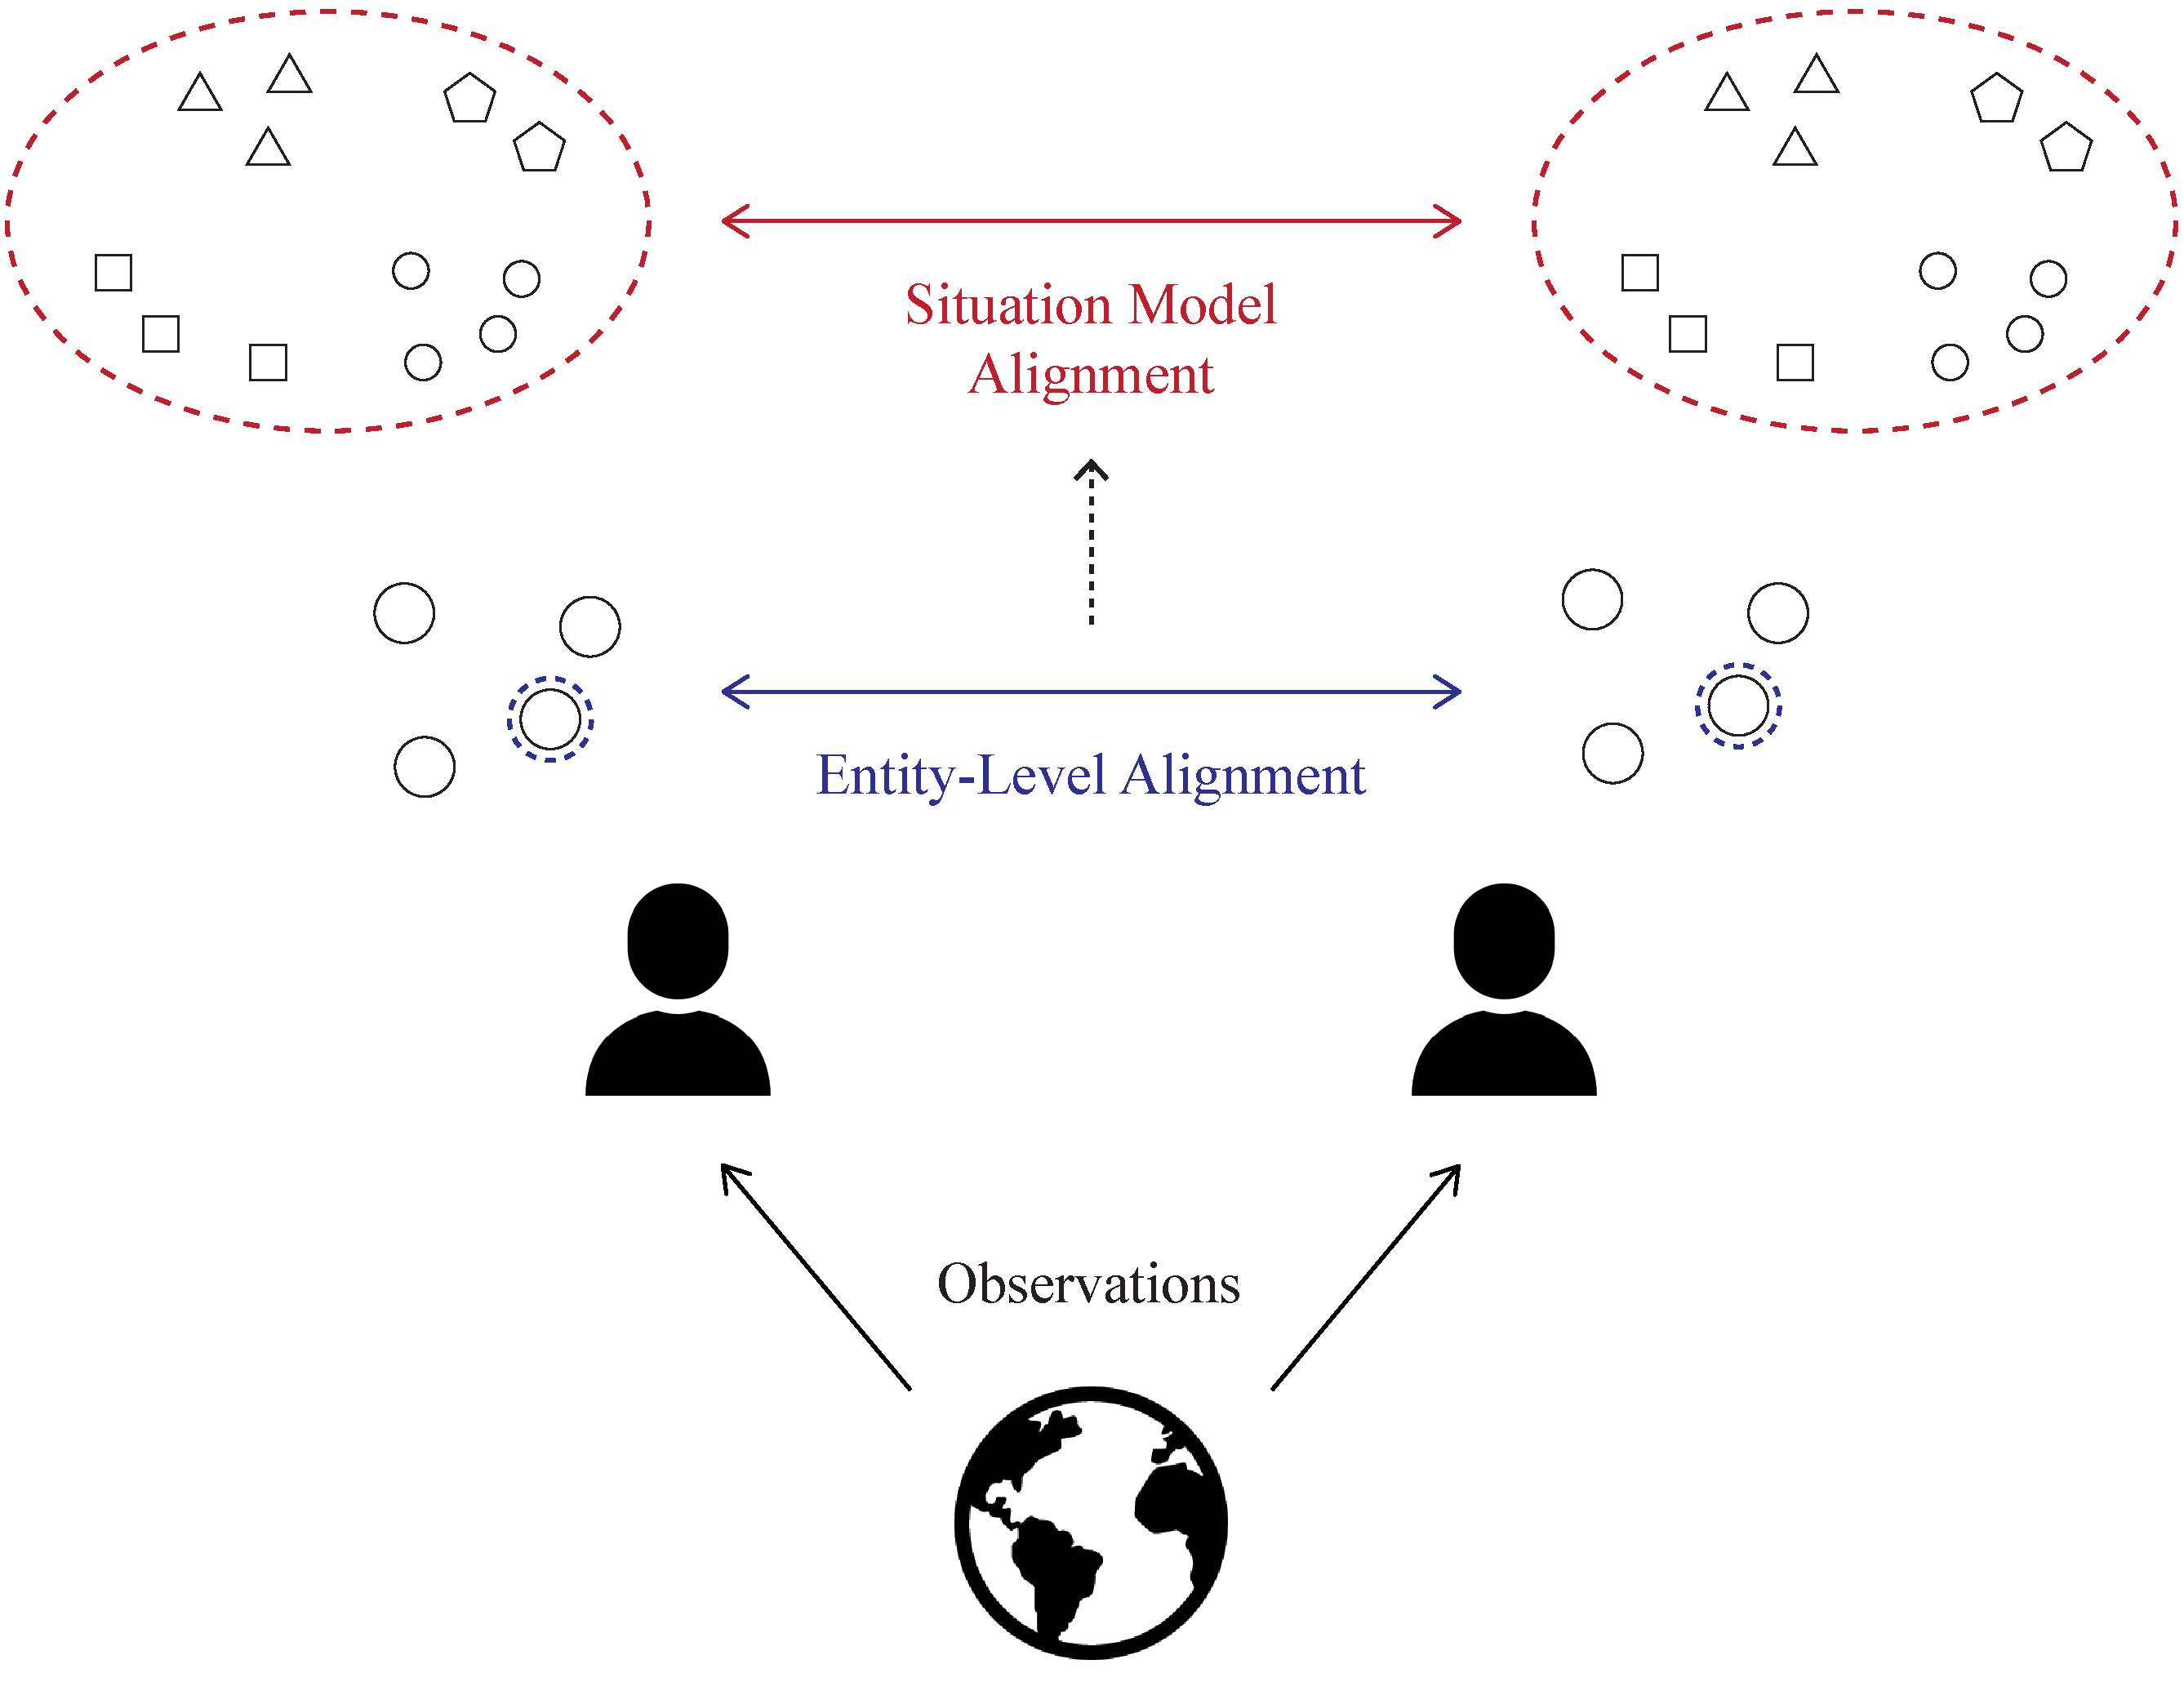
\includegraphics[width=\textwidth]{situation_models.pdf}
\caption{An illustration of the current task formulations (\textit{entity-level alignment}) and the desired task formulations (\textit{situation model alignment}).
}
\label{07_fig:situation_model_alignment}
\end{figure*}

If we were to study fully advanced common grounding, we expect task formulations which require the alignment of entire situation models will be critical (as illustrated in Figure \ref{07_fig:situation_model_alignment}). To be specific, we need appropriate task designs which require alignment at all conceivable dimentions (not only \textit{space} and \textit{time} but also \textit{causality}, \textit{intentionality} and \textit{protagonists}). We also need task formulations which enable reliable evaluation of the accurate situation model alignment (rather than entity-level alignment). These requirements are much more demanding, but there are several potential solutions. One approach is to carefully design questions to test whether the situation models are correctly aligned, as similarly proposed in the reading comprehension literature \citep{sugawara-etal-2021-benchmarking}. For instance, after (or in the middle of) the conversation, we can ask each interlocutor some questions that require the answers to be coordinated: e.g. ``what event do you (and your partner) expect if the player had not scored an own goal?'' or ``what do you (and your partner) believe the intention of the player was?'', where alignment of situation models at the \textit{causal} (\textit{counterfactual}) dimension and \textit{intentionality} dimension is required, respectively. We leave the exploration of specific task designs, evaluation metrics and dataset collection as an important avenue of future work.

\section{Improving Common Grounding}
\label{07_sec:advanced_common_grounding_models}

Throughout this thesis, we have proposed several approaches to improve common grounding in data-driven dialogue systems: such as multi-task training with reference resolution (Chapter \ref{04_chp:interpretation}) and pretraining on a related dataset (Chapter \ref{06_chp:task_generalization}). However, we can conceive of three major approaches to further improve their performances.

One approach is to make the model learn from the task success and failure based on \textit{reinforcement learning} \citep{sutton2018reinforcement}. This can be realized through an actual interaction with the human players (e.g. crowd workers) but also by repeatedly playing the task against itself, known as \textit{selfplay} \citep{silver2016mastering}. The latter approach is much cheaper and more scalable, hence widely applied in dialogue domains with symmetric speaker roles \citep{lewis-etal-2017-deal,DBLP:conf/icml/YaratsL18,jang2020bayes}. The upside is that we can expect the models to learn to avoid ineffective strategies, such as underspecification and premature guessing. However, the downside is that they can potentially diverge from natural language \citep{kottur-etal-2017-natural}, making communication with humans more difficult and unreliable.

We also expect the incorporation of \textit{pragmatic reasoning} to be a fruitful area of future research. One representative approach is the \textit{Rational Speech Act} (\textit{RSA}) framework \citep{Goodman2016PragmaticLI}, which has been applied in both continuous \citep{monroe2017colors,mcdowell-goodman-2019-learning} and partially-observable domains \citep{Hawkins2021TheDO}. However, application in \textit{interactive} and \textit{dynamic} domains would involve additional complexities that need to be taken into account, such as the dependencies on dialogue history and previous common ground.

Finally, we can study wider variety of model architectures and pretraining datasets. For instance, we have considered the observations to be in \textit{structured} format (e.g. based on xy coordinates), but we can also extract \textit{raw} visual features by directly treating them as images or videos \citep{suhr2017corpus,iki2020language}. In the latter case, we can apply various techniques from CV and NLP, including image/video processing methods \citep{Carreira2017QuoVA,wang2018non,dosovitskiy2021an}, vision-language grounding models \citep{lu2019vilbert,le-etal-2020-bist} and pretraining on large-scale, open domain datasets \citep{krishna2017visual,sharma-etal-2018-conceptual}. Note that the entity-level representation of the observation (required in our baselines) can be obtained from raw visual features as well, e.g. by utilizing the object detectors \citep{NIPS2015_14bfa6bb,redmon2016you} and trackers \citep{tracktor_2019_ICCV,wang2020towards}. Lastly, we can replace the \textit{dialogue encoders} of our baselines based on the transformer architectures \citep{NIPS2017_3f5ee243}, which have become the mainstream approch in language and dialogue modelling \citep{devlin-etal-2019-bert,lewis-etal-2020-bart,zhang-etal-2020-dialogpt}.


\section{Real-World Applications}
\label{07_sec:real_world_applications}

Finally, we'd like to discuss the impact of our work on real-world applications. While our resources (OneCommon Corpus and Dynamic-OneCommon Corpus) are currently restricted to synthetic settings, the general ideas and strategies we have investigated are fundamental in many practical applications.

For instance, consider the case of \textit{item retrieval}, such as recommending a furniture by soliciting the user preferences (as in \citealp{moon-etal-2020-situated}). Since the user's taste can be very precise, this requires dealing with subtle nuances like ``do you have something that's \textit{a little more} white and round shaped?'' or partial replacements like ``I like its materials \textit{except for} the backrest''. Dealing with such expressions are critical under \textit{continuous} context and can be studied rigorously based on OneCommon Corpus. In addition, this setting can become \textit{partially-observable} in case the actual furniture is not visible to the user, e.g. when the item is out of stock or the user is talking to speech-based devices. On such occasions, the system needs to take into account the possibility of various misunderstandings to make the transaction accurate and reliable.

We can also illustrate the importance of \textit{dynamic} context based on a navigation task in commonplace environments, such as finding a lost child in an urban city. In reality, the \textit{target entity} (the child) may not stay in one place, so the routing directions can no longer be fixed and need to be \textit{updated} accordingly (as in ``now head more to the west'' or ``go back to the previous block''). Furthermore, the \textit{landmark entities} may not be stationary either and could be ephemeral (as in ``following the group of travelers'' or ``in the middle of the crowd''). The task may be trivial if the child is conspicuous with few distractors, but otherwise (e.g. with many pedestrians around), the descriptions need to be precise and distinguishing (as in ``wearing \textit{a little} darker shirt'', ``walking \textit{right} towards the station''). In order to study such (nuanced and pragmatic) spatio-temporal expressions and references to previous common ground, we expect Dynamic-OneCommon Corpus to be an essential proving ground for developing and analyzing various models.\footnote{Unfortunately, most of the existing navigation tasks focus on \textit{static} environments (e.g. static targets and landmarks): see Section \ref{06_sec:related_work} for further discussions.}

Overall, we expect our contributions to be critical for promoting reliable collaboration in real-world environments, which involve the advanced settings of \textit{continuous}, \textit{partially-observable} and \textit{dynamic} context.






\chapter{Conclusion}
\label{08_chp:conclusion}

Developing systems that can understand and communicate in natural language is an ultimate goal of NLP and AI research. In this thesis, we focused on the aspect of common grounding as the key requisite for truly reliable conversation.

In Chapter \ref{02_chp:literature_review}, we gave an overview of the existing research related to common grounding. First, we introduced the theoretical foundations of common grounding in philosophy, mathematical logic and pyscholinguistics. Then, we explained the computational approaches to common grounding, including the general literature on dialogue system engineering. Finally, we discussed the important links to the problem of symbol grounding, which is deeply related to common grounding (especially in situated dialogues). Overall, we clarified the limitations of existing research and emphasized the importance of our research in these broader contexts.

In Chapter \ref{03_chp:task_formulation}, we introduced a novel task setting under continuous and partially-observable context. Following this idea, we designed a minimal collaborative reference task and developed OneCommon Corpus containing 6,760 dialogues. Through our dataset analysis, we verified advanced common grounding required in this setting, such as the  collaborative resolution of complex ambiguity, uncertainty and misunderstandings. As a preliminary experiment, we evaluated a simple baseline model on the target selection task and verified the difficulty of even recognizing the common ground. 

In Chapter \ref{04_chp:interpretation}, we proposed a method of decomposing common grounding based on its subtask of reference resolution. Based on our simple and generic framework, we annotated 5,191 successful dialogues from OneCommon Corpus which capture genuine ambiguity while maintaining reliability. Our dataset analysis demonstrated the importance of our annotation for interpreting the intermediate process of common grounding. Finally, we built end-to-end dialogue systems as the baselines for our proposed dataset. Our annotation helped improve and interpret their common grounding strategies, but substantial room remained for further improvement.

In Chapter \ref{05_chp:analysis}, we conducted further analyses of OneCommon Corpus based on spatial expressions. Specifically, we leveraged the existing annotation of referring expressions to annotate their spatial predicates (including modifications) efficiently and reliably. Although our annotation size is relatively small (600 dialogues), we revealed important linguistic structures in our dataset, i.e. predicate-argument structure, modification and ellipsis. Finally, through our extensive experiments, we showed how and where the current baselines struggle in capturing such precise structures.

In Chapter \ref{06_chp:task_generalization}, we further take into account the task setting under dynamic environments. To evaluate and analyze the ability of mainining common ground, we formulated the sequential collaborative reference task and collected Dynamic-OneCommon Corpus containing 5,617 dialogues. Our dataset analyses demonstrated sophisticated strategies required in this setting, such as the usage of spatio-temporal expressions and references to previous common ground. In our experiments, we conducted thorough evaluation of the end-to-end dialogue systems based on this dataset. Overall, we showed that there remains significant room left for improvement due to the requirement of even more advanced common grounding strategies.

In Chapter \ref{07_chp:discussion}, we briefly explored the future prospects of our research. In terms of the task design methodologies, we expect the view of \citet{pickering2004toward} will be crucial for the next-generation task formulations reflecting fully advanced common grounding. Next, we gave an overview of the promising directions to further improve the model performances in terms of common grounding. Finally, we illustrated several potential applications of our contributions in the practical, real-world settings.

All together, we expect this thesis to be a fundamental basis for realizing truly reliable communication between humans and computers. All of our resources are publicly available to facilitate future research, and we hope they will encourage further analyses and improvements of dialogue systems in terms of advanced common grounding.



%-------------------
\bibliographystyle{plainnat}
\bibliography{myref}
%-------------------
\end{document}
